\documentclass[a4paper, 11pt, oneside, polutonikogreek, german]{article}
\usepackage{kmath, kerkis}
\usepackage[T1]{fontenc}
% Load encoding definitions (after font package)
\usepackage[dvipsnames]{xcolor}
\usepackage{eso-pic,graphicx}
\usepackage[top=53mm, bottom=53mm, outer=45mm, inner=45mm]{geometry}
\setlength{\columnsep}{90pt}
\usepackage{textalpha}
\usepackage{bbding}
\usepackage{listings}
\lstset{basicstyle=\ttfamily}
\usepackage{wasysym}

% Babel package:
\usepackage[german]{babel}

% With XeTeX$\$LuaTeX, load fontspec after babel to use Unicode
% fonts for Latin script and LGR for Greek:
\ifdefined\luatexversion \usepackage{fontspec}\fi
\ifdefined\XeTeXrevision \usepackage{fontspec}\fi

% "`Lipsiakos"' italic font `cbleipzig`:
\newcommand*{\lishape}{\fontencoding{LGR}\fontfamily{cmr}%
		 \fontshape{li}\selectfont}
\DeclareTextFontCommand{\textli}{\lishape}
\usepackage{sectsty}
\usepackage[titles]{tocloft}

\sectionfont{\large}
\subsectionfont{\normalsize}
\subsubsectionfont{\small}

\usepackage{setspace}
\onehalfspacing
\usepackage{booktabs}
\setlength{\emergencystretch}{15pt}
\usepackage{fancyhdr}
\usepackage{microtype}
\usepackage{graphicx}
\graphicspath{ {./ } }
\usepackage[figurename=]{caption}
\usepackage{float}
% change color of text, example replace all \color{Goldenrod} with \color{lightgray}
%\definecolor{lightblue}{RGB}{22, 85, 233}


\makeatletter % change only the display of \thepage, but not \thepage itself:
\patchcmd{\ps@plain}{\thepage}{\bfseries\large\color{Black}{\thepage}}{}{}
\makeatother

\color{Black}

\begin{document}
\renewcommand{\thefigure}{{\bfseries\arabic{figure}}}
\renewcommand\thefootnote{\tiny{\arabic{footnote}}}
\let\oldfootnote\footnote
    \renewcommand{\footnote}[1]{\oldfootnote{\bfseries\footnotesize#1}}
    
\bfseries
\pagestyle{plain} % after changing a pagestyle command, it's necessary to invoke it explicitly
\AddToShipoutPictureBG{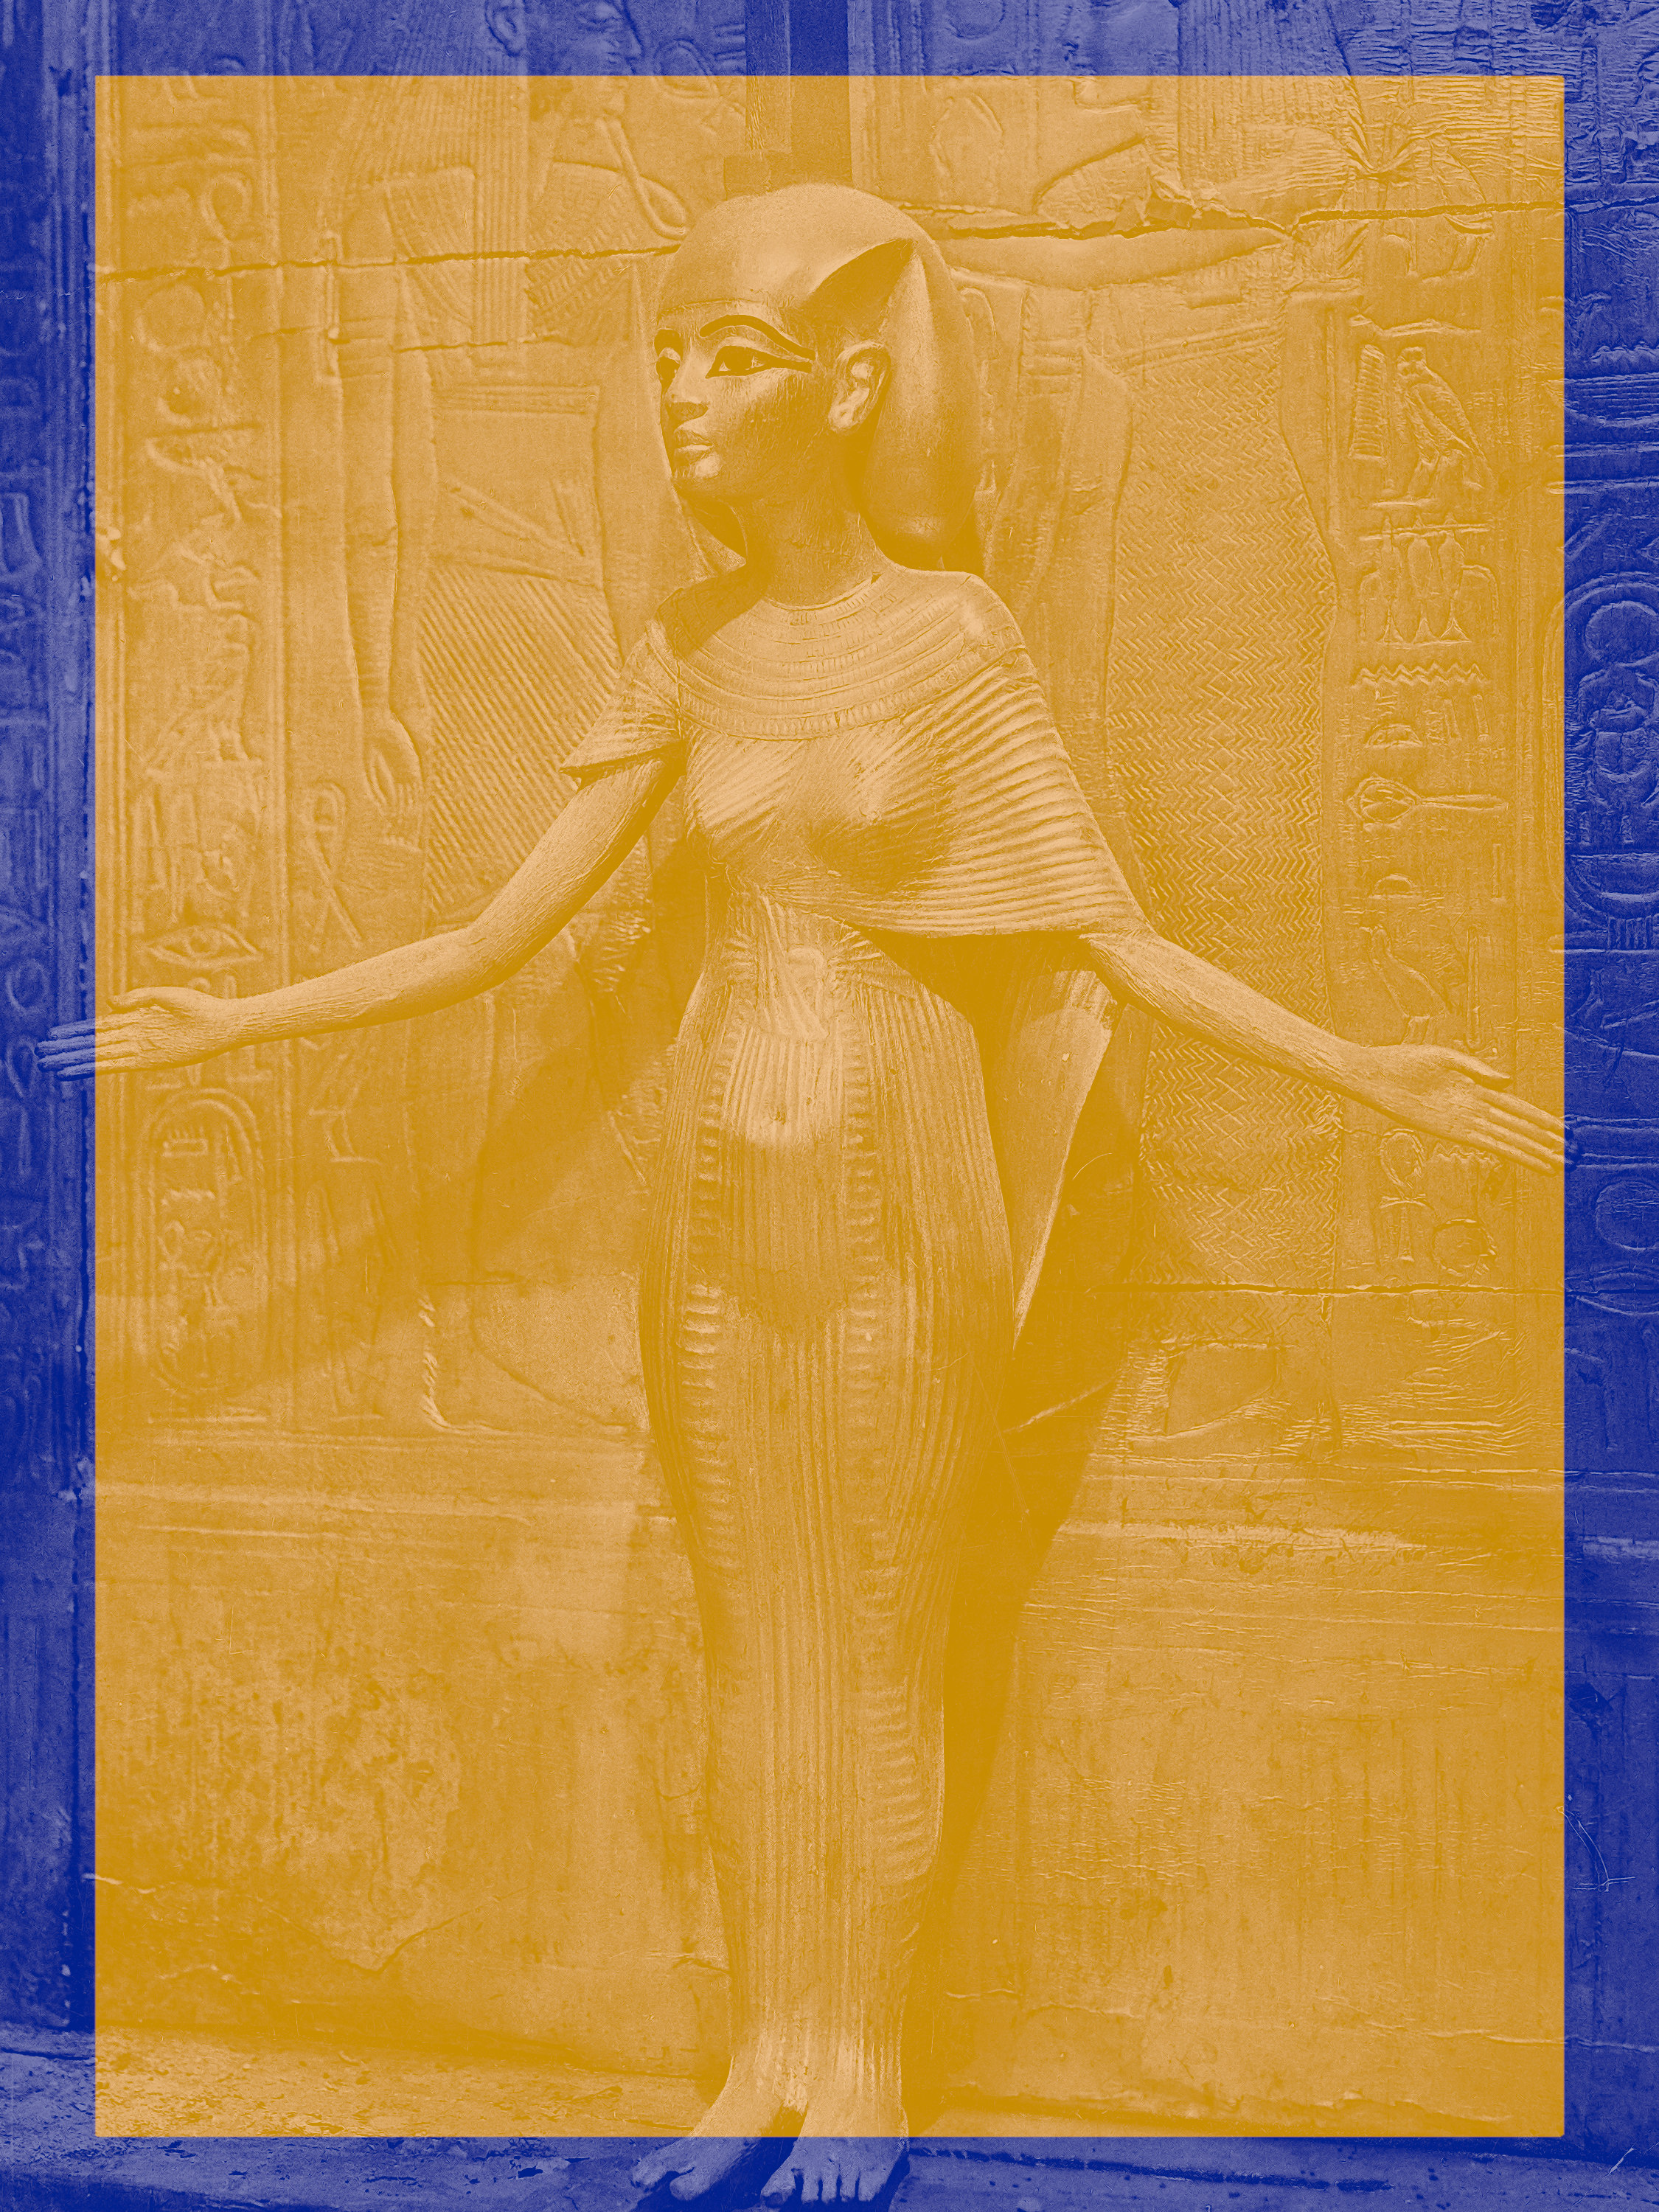
\includegraphics[width=\paperwidth,height=\paperheight]{custom2.jpeg}}
\begin{titlepage} % Suppresses headers and footers on the title page
	\centering % Centre everything on the title page
	%\scshape % Use small caps for all text on the title page

	%------------------------------------------------
	%	Title
	%------------------------------------------------

	\rule{\textwidth}{1.6pt}\vspace*{-\baselineskip}\vspace*{2pt} % Thick horizontal rule
	\rule{\textwidth}{0.4pt} % Thin horizontal rule
	
	\vspace{1\baselineskip} % Whitespace above the title
	
	{\Huge Περὶ Ἴσιδος καὶ Ὀσίριδος}
	
	\vspace{1\baselineskip} % Whitespace above the title

	\rule{\textwidth}{0.4pt}\vspace*{-\baselineskip}\vspace{3.2pt} % Thin horizontal rule
	\rule{\textwidth}{1.6pt} % Thick horizontal rule
	
	\vspace{1\baselineskip} % Whitespace after the title block
	
	%------------------------------------------------
	%	Subtitle
	%------------------------------------------------
	
	{\Large Πλούταρχος}
 
        \vspace{0.5\baselineskip}
	
	\vspace*{1\baselineskip} % Whitespace under the subtitle
	
        {\scshape \normalsize } % Subtitle or further description

	%------------------------------------------------
	%	Editor(s)
	%------------------------------------------------
        \vspace*{\fill}    

	\vspace{1\baselineskip}

	{\small\scshape 1778}
	
	{\small\scshape{Impensis Gotthelf Theophil Georgi}}
	
	\vspace{0.5\baselineskip} % Whitespace after the title block

        {\scshape Internet Archive Online Edition}% Publication year}
    
	{\small CC Αναφορά-Μη Εμπορική Χρήση 4.0} % Publisher
\end{titlepage}
\setlength{\parskip}{1mm plus1mm minus1mm}
\clearpage
\large
\paragraph{1.}
Πάντα μὲν, ὦ Κλέα,\footnote{ὦ Κλέα] Quamuis nomen apud Plutarchum T. 1. Opp. philos. p. 432. ed. \emph{H. Stephani} etiam occurrat, ubi eidem foeminae libellum de mulierum virtutibus dedicat; videtur tamen cum analogia Graecorum nominum foemininorum haud congruere. Κλεᾶς est nomen masculinum pro Κλέανδρος, unde vocat. Κλεᾶ pro Κλέανδρε. Foemininum ergo nequit esse Κλέα, sed est Κλεαρέτη. quod haud scio an Plutarchus dederit. \emph{Reiske.}} δεῖ τἀγαθὰ τοὺς νοῦν ἔχοντας αἰτεῖσθαι παρὰ τῶν θεῶν, μάλιστα δὲ τῆς περὶ αὐτῶν ἐπιστήμης, ὅσον ἐφικτόν ἐστιν ἀνθρώποις μετιόντες, εὐχόμεθα τυγχάνειν παρ' αὐτῶν ἐκείνων\footnote{ἐκείνης. redit enim ad ἐπιστήμην. \emph{Reiske.}} · ὡς οὐθὲν ἀνθρώπῳ λαβεῖν μεῖζον, οὐ χαρίσασθαι θεῷ σεμνότερον\footnote{σεμνότερον ὂν ἀληθείας. \emph{Reiske.}} ἀληθείας. τὰ ἄλλα μὲν γὰρ\footnote{τὰ μὲν γὰρ ἄλλα. \emph{Reiske.}} ἀνθρώποις ὁ θεὸς, ὧν δέονται, δίδωσιν, οἰκεῖα\footnote{οἰκεῖα κεκτ.] Videtur sensum absurdum gignere, legi autem, δίδωσιν οὐκ οἰκεῖα κεκτημένος. \emph{Xylander.}} κεκτημένος ταῦτα καὶ χρώμενος.\footnote{Salmasius κεκτημένοις et χρωμένοις emendavit. \emph{Reiske.}} οὐ γὰρ ἀργύρῳ καὶ χρυσῷ μακάριον τὸ θεῖον, οὐδὲ βρονταῖς καὶ κεραυνοῖς ἰσχυρὸν, ἀλλ' ἐπιστήμῃ καὶ φρονήσει, καὶ τοῦτο κάλλιστα πάντων Ὅμηρος, ὧν εἴρηκε,\footnote{Comma post εἴρηκε delend. \emph{omnium, quae de diis dixit.} \emph{Reiske.}} περὶ θεῶν ἀναφθεγξάμενος ·
\begin{quotation}\normalsize
Ἦ μὰν ἀμφοτέροισιν ὁμὸν γένος ἠδ' ἴνα πάτρη,

Ἀλλὰ Ζεὺς πρότερος γεγόνει, καὶ πλείονα ᾔδει.
\end{quotation}
\paragraph{}
σεμνοτέραν ἀπέφῃνε τὴν τοῦ Διὸς ἡγεμονίαν ἐπιστήμς καὶ σοφίας,\footnote{Sic distinguo et lego: ἡγεμονίαν, ὑπ' ἐπιστήμης καὶ, σοφίας πρεσβ. \emph{Reiske.}} πρεσβυτέραν οὖσαν. οἶμαι δὲ καὶ τῆς αἰωνίου ζωῆς, ἣν ὁ θεὸς εἴληχεν, εὔδαιμον εἶναι τὸ τῇ γνώσει μὴ προαπολιπεῖν τὰ γινόμενα\footnote{τῶν γινομένων. \emph{Reiske.}} · τοῦ δὲ γινώσκειν τὰ ὄντα, καὶ φρονεῖν ἀφαιρεθέντος, οὐ βίον, ἀλλὰ χρόνον εἶναι τὴν ἀθανασίαν.

\paragraph{2.}
διὸ θειότητος ὄρεξις ἐστιν ἡ τῆς ἀληθείας, μάλιστα δὲ τῆς περὶ θεῶν ἔφεσις, ὥσπερ ἀνάληψιν ἱερῶν τὴν μάθησιν ἔχουσα καὶ τὴν ζήτησιν. ἁγνείας τε πάσης καὶ νεωκορίας ἔργον ὁσιώτερον, οὐχ ἥκιστα δὲ τῇ θεῷ ταύτῃ κεχαρισμένον, ἣν σὺ θεραπεύεις ἐξαιρέτως σοφὴν καὶ φιλόσοφον οὖσαν, ὡς τοὔνομά τε\footnote{f. ἧς τοὔνομά γε φράζειν. \emph{Reiske.}} φράζειν ἔοικε παντὸς μᾶλλον αὐτῇ τὸ εἰδέναι καὶ τὴν ἐπιστήμην προσήκουσαν. Ἑλληνικὸν γὰρ ἡ Ἶσίς ἐστι, καὶ ὁ Τυφὼν πολέμιος τῇ θεῷ,\footnote{Distinguo et lego: Τυφὼν, πολέμιος τῇ θεῷ ὢν. significat Typhonis quoque nomen Graecae originis esse. \emph{Reiske.}} καὶ δ' ἄγνοιαν καὶ ἀπάτην τετυφωμένος, καὶ διασπῶν καὶ ἀφανίζων τὸν ἱερὸν λόγον, ὃν ἡ θεὸς συνάγει καὶ συντίθησι, καὶ παραδίδωσι τοῖς τελουμένοις θειώσεως,\footnote{διὰ θειώσεως. \emph{per sanctificationem.} \emph{Reiske.}} σώφρονι μὲν ἐνδελεχῶς διαίτῃ, καὶ βρωμάτων πολλῶν καὶ ἀφροδισίων ἀποχαῖς κωλυούσαις τὸ ἀκόλαστον καὶ φιλήδονον, ἀθρύπτους δὲ καὶ στεῤῥὰς ἐν ἱεροῖς λατρείας ἐθιζούσης ὑπομένειν, ὧν τέλος ἐστὶν ἡ τοῦ πρώτου καὶ κυρίου καὶ νοητοῦ γνῶσις, ὃν ἡ θεὸς παρακαλεῖ ζητεῖν παρ' αὐτῇ καὶ μετ' αὐτῆς ὄντα καὶ συνόντα.\footnote{καὶ συνόντα videri queat redundare. sed respicit ad uxoris cum marito consuetudinem coniugalem. \emph{Reiske.}} τοῦ δ' ἱεροῦ τοὔνομα καὶ σαφῶς ἐπαγγέλλεται καὶ γνῶσιν καὶ εἴδησιν τοῦ ὄντος. ὀνομάζεται γὰρ Ἴσειον ὡς εἰσόμένον\footnote{ὡς εἰσόμενον] legi εἰσόμενοι. Voce \emph{ens} utendum fuit, nisi obscuritati debui caliginem addere. \emph{Xylander.} εἰσομένων ipse quoque conieceram, antequam Bentleyum, Baxterum, Marklandum idem sensisse intelligerem. subauditur ἡμῶν. \emph{ac si cognituri essemus.} \emph{Reiske.}} τὸ ὂν, ἂν μετὰ λόγου καὶ ὁσίως εἰς τὰ ἱερὰ παρέλθωμεν τῆς θεοῦ.

\paragraph{3.}
ἔτι πολλοὶ μὲν Ἑρμοῦ, πολλοὶ δὲ Προμηθέως ἱστορήκασιν αὐτὴν θυγατέρα · ὧν\footnote{Aut ὧν delendum, aut cum ὡς mutandum, aut deinceps legendum νομίζομεν. \emph{Reiske.}} τὸ μὲν ἕτερον, σοφίας καὶ προνοίας, Ἑρμῆν δὲ γραμματικῆς καὶ μουσικῆς εὑρετὴν νομίζοντες. Διὸ καὶ τῶν Ἑρμουπόλει Μουσῶν τὴν προτέραν Ἶσιν ἅμα καὶ δικαιοσύνην καλοῦσι σοφίαν, ὥσπερ εἴρηται, καὶ δεικνύουσαν\footnote{f. εἴρηται, οὖσαν, καταδεικνύουσαν. \emph{Reiske.}} τὰ θεῖα τοῖς ἀληθῶς καὶ δικαίως ἱεραφόροις\footnote{ἱεραφόροις rectum est. nam in talibus α pari iure locoque est atque ο, ut βιβλιαφόρος et βιβλιοφόρος. \emph{Reiske.}} καὶ ἱεροστόλοις προσαγορευομένοις · οὗτοι δέ εἰσὶν οἱ τὸν ἱερὸν λόγον περὶ θεῶν πάσης καθαρεύοντα δεισιδαιμονίας καὶ περιεργίας ἐν τῇ ψυχῇ φέροντες, ὥσπερ ἐν κίστῃ, καὶ περιστέλλοντες · τὰ μὲν, μέλανα\footnote{τὰ μὲν μέλανα.] Deest aliquid. Post aliquot versus in τούτους ὅταν νόμῳ si deleatur ὅταν, sensus constabit. \emph{Xylander.} περιστέλλοντες μὲν τὰ μέλανα. \emph{Reiske.}} καὶ σκιώδη, τὰ δὲ, φανερὰ καὶ λαμπρὰ τῆς περὶ θεῶν ὑποδηλοῦντα\footnote{Nullus dubito, rectum eos vidisse, qui ὑποδηλοῦντες, id est προδηλοῦντες, προφαίνοντες, emendarunt. \emph{ostendentes.} \emph{Reiske.}} οἰήσεως, οἷα καὶ περὶ τὴν ἐσθῆτα τὴν ἱερὰν ἀποφαίνεται. διὸ καὶ τὸ κοσμεῖσθαι τούτοις τοὺς ἀποθανόντας Ἰσιακοὺς, σύμβολόν ἐστι τοῦ τε τὸν λόγον εἶναι μετ' αὐτῶν, καὶ τοῦτον ἔχοντας, ἄλλο δὲ μηδὲν, ἐκεῖ βαδίζειν. οὔτε γὰρ φιλοσόφους πωγωνοτροφίαι, ὦ Κλέα, καὶ τριβωνοφορίαι ποιοῦσιν οὔτ' Ἰσιακοὺς αἱ λινοστολίαι καὶ ξύρησις\footnote{ξυρήσεις in plurali. \emph{Reiske.}} · ἀλλὰ Ἰσιακός ἐστιν ὡς ἀληθῶς ὁ τὰ δεικνύμενα καὶ δρώμενα περὶ τοὺς θεοὺς τούτους, ὅταν νόμῳ παραλάβῃ, λόγῳ ζητῶν, καὶ φιλοσοφῶν περὶ τῆς ἐν αὐτοῖς ἀληθείας.

\paragraph{4.}
ἐπεὶ τούς γε πολλοὺς καὶ τὸ κοινότατον τοῦτο καὶ σμικρότατον λέληθεν, ἐφ' ὅτῳ τὰς τρίχας οἱ ἱερεῖς ἀποτίθενται καὶ λινᾶς ἐσθῆτας φοροῦσιν, οἱ μὲν οὐδόλως\footnote{f. οἱ μὲν γὰρ οὐδ' ὅλως. \emph{Reiske.}} φροντιζουσιν εἰδέναι περὶ τούτων · οἱ δὲ τῶν μὲν ἐρίων ὥσπερ τῶν κρεῶν, σεβομένους τὸ πρόβατον ἀπέχεσθαι λέγουσι, ξύρεσθαι δὲ τὰς κεφαλὰς διὰ τὸ πένθος, φορεῖν δὲ τὰ λινᾶ διὰ τὴν χρόαν, ἣν τὸ λῖνον ἀνθοῦν ἀνίησι τῇ περιεχούσῃ τὸν κόσμον αἰθερίῳ χαροπότητι προσεοικυῖαν. ἡ δ' ἀληθὴς αἰτία μία πάντων ἐστί · καθαροῦ γὰρ (ᾗ φησιν ὁ Πλάτων) οὐ θεμιτὸν ἅπτεσθαι μὴ καθαρῷ. περίσσωμα δὲ τροφῆς καὶ σκύβαλον οὐδὲν ἁγνὸν, οὐδὲ καθαρόν ἐστιν · ἐκ δὲ περιττωμάτων ἔρια καὶ λάχναι, καὶ τρίχες καὶ ὄνυχες ἀναφύονται καὶ βλαστάνουσι. γελοῖον οὖν ἦν, τὰς μὲν αὐτῶν τριχας ἐν ταῖς ἁγνείαις ἀποτίθεσθαι ξυρωμένους καὶ λειαινομένους πᾶν ὁμαλῶς τὸ σῶμα, τὰς δὲ τῶν θρεμμάτων ἀμπέχεσθαι καὶ φορεῖν. καὶ γὰρ τὸν Ἡσίοδον οἴεσθαι δεῖ, λέγοντα ·
\begin{quotation}\normalsize
Μηδ' ἀπὸ πεντόζοιο θεῶν ἐν δαιτὶ θαλείῃ

Αὖον ἀπὸ χλωροῦ τάμνειν αἴθωνι σιδήρῳ ·
\end{quotation}
\paragraph{}
διδάσκειν, ὅτι δεῖ καθαροὺς τῶν τοιούτων γενομένους ἑορτάζειν, οὐκ ἐν αὐταῖς ταῖς ἱερουργίαις χρῆσθαι καθάρσει καὶ ἀφαιρέσει τῶν περιττωμάτων. τὸ δὲ λῖνον φύεται μὲν ἐξ ἀθανάτου τῆς γῆς, καὶ καρπὸν ἐδώδιμον ἀναδίδωσι, λιτὴν δὲ παρέχει καὶ καθαρὰν ἐσθῆτα, καὶ τῷ σκέποντι\footnote{Humanum aliquid hic loci passus est Cl. Marklandus. τῷ σκέποντι idem est, atque ἐν (vel ἅμα) τῷ σκέποντι. \emph{quamuis tegat hominem, non tamen ideo gravat.} \emph{Reiske.}} μὴ βαρύνουσαν, εὐάρμοστον δὲ πρὸς πᾶσαν ὥραν · ἥκιστα δὲ φθειροποιὸν, ὡς λέγουσι · περὶ ὧν ἕτερος λόγος.

\paragraph{5.}
οἱ δὲ ἱερεῖς οὕτω δυσχεραίνουσι τὴν τῶν περιττωμάτων φύσιν, ὥστε μὴ μόνον παραιτεῖσθαι τῶν ὀσπρίων τὰ πολλὰ, καὶ τῶν κρεῶν τὰ μήλεια καὶ ὕεια, πολλὴν ποιοῦντα περίττωσιν, ἀλλὰ καὶ τοὺς ἅλας τῶν σιτίων ἐν ταῖς ἁγνείαις ἀφαιρεῖν · ἄλλας τε πλείονας αἰτίας ἔχοντας, καὶ τὸ ποτικωτέρους καὶ βρωτικωτέρους ποιεῖν ἐπιθίγοντας τὴν ὄρεξιν. τὸ γὰρ (ὡς Ἀρισταγόρας ἔλεγε) διὰ τὸ πηγνυμένοις πολλὰ τῶν μικρῶν ζώων ἐναποθνήσκειν ἁλισκόμενα μὴ καθαροὺς λογίζεσθαι τοὺς ἅλας, εὔηθές ἐστι. λέγονται\footnote{f. εὒηθές ἐστι λέγειν. λέγονται. \emph{Reiske.}} δὲ καὶ τὸν Ἆπιν ἐκ φρέατος ἰδίου ποτίζειν, τοῦ δὲ Νείλου παντάπασιν ἀπείργειν, οὐ μιαρὸν ἡγουμένος\footnote{Facio cum Marklando ἡγούμενοι suadente. \emph{Reiske.}} τὸ ὕδωρ διὰ τὸν κροκόδειλον, ὡς ἔνιοι νομίζουσιν · (οὐδὲν γὰρ οὕτω τιμὴ\footnote{οὕτω τίμιον, aut οὕτως ἐν τιμῇ. \emph{Reiske.}} Αἰγυπτίοις, ὡς ὁ Νεῖλος) ἀλλὰ πιαίνειν δοκεῖ καὶ μάλιστα πολυσαρκίαν ποιεῖν τὸ Νειλῶον ὕδωρ πινόμενον. οὐ βούλονται δὲ τὸν Ἆπιν οὕτως ἔχειν, οὐδὲ ἑαυτοὺς, ἀλλὰ εὐσταλῆ καὶ κοῦφα ταῖς ψυχαῖς περικεῖσθαι τὰ σώματα, καὶ μὴ πιέζειν, μηδὲ καταθλίβειν ἰσχύοντι τῷ θνητῷ, καὶ βαρύνοντι τὸ θεῖον.

\paragraph{6.}
οἶνον δὲ οἱ μὲν ἐν Ἡλίου πόλει θεραπεύοντες τὸν θεὸν, οὐκ εἰσφέρουσι τοπαράπαν εἰς τὸ ἱερόν, ὡς οὐ προσῆκον ὑμέρας\footnote{Rectum esse ἡμέρας, et Squirii coniectura nil opus esse sequentia euincunt, et de solis sacerdotibus sermonem hic esse monstrant praemissa; quapropter necesse non est sacerdotum nomen hic iterum inculcari. \emph{Reiske.}} πίνειν, τοῦ κυρίου καὶ βασιλέας ἐφορῶντος · οἱ δ' ἄλλοι χρῶνται μὲν, ὀλίγῳ δέ. πολλὰς δ' ἀοίνους ἁγνείας ἔχουσιν, ἐν αἷς φιλοσοφοῦντες καὶ μανθάνοντες καὶ διδάσκοντες τὰ θεῖα διατελοῦσιν. οἱ δὲ βασιλεῖς καὶ μετρητὸν ἔπινον ἐκ τῶν ἱερῶν γραμμάτων (ὡς Ἑκαταῖος ἱστόρηκεν) ἱερεῖς ὄντες · ἤρξαντο δὲ πίνειν ἀπὸ Ψαμμητίχου, πρότερον δ' οὐκ ἔπινον οἶνον, οὐδὲ ἔσπενδον, ὡς φίλιον θεοῖς, ἀλλ' ὡς αἷμα τῶν πολεμησάντων ποτὲ τοῖς θεοῖς, ἐξ ὧν οἴονται πεσόντων καὶ τῇ γῇ συμμιγέντων ἀμπέλους γενέσθαι. διὸ καὶ τὸ μεθύειν ἔκφρονας ποιεῖ καὶ παραπλῆγας, ἅτε δὴ τῶν προγόνων τοῦ αἵματος ἐμπιπλαμένους. ταῦτα μὲν οὖν Εὔδοξος ἐν τῇ δευτέρᾳ τῆς περιόδου λέγεσθαί φησιν οὕτως ὑπὸ τῶν ἱερέων.

\paragraph{7.}
ἰχθύων δὲ θαλαττίων, πάντες μὲν οὐ πάντων, ἀλλ' ἐνίων ἀπέχονται. καθάπερ ὀξυρυγχῖται τῶν ἀπ' ἀγκίστρου. σεβόμενοι γὰρ τὸν ὀξύρυγχον ἰχθὺν, δεδίασι, μή ποτε τὸ ἄγκιστρον οὐ καθαρόν ἐστιν ὀξυρύγχου περιπεσόντος αὐτῷ. Συηνῖται δὲ φάγρου · δοκεῖ γὰρ ἐπιόντι τῷ Νείλῳ συνεπιφαίνεσθαι, καὶ τὴν αὔξησιν ἀσμένοις φράζειν αὐτάγγελος ὁρώμενος. οἱ δ' ἱερεῖς ἀπέχονται πάντων · πρώτου δὲ μηνὸς ἐνάτῃ τῶν ἄλλων Αἰγυπτίων ἑκάστου πρὸ τῆς αὐλείου θύρας ὀπτὸν ἰχθὺν κατεσθίοντος, οἱ ἱερεῖς οὐ γεύονται μὲν, κατακαίουσι δὲ πρὸ τῶν θυρῶν τοὺς ἰχθῦς · δύο λόγους ἔχοντες, ὧν τὸν μὲν ἱερὸν καὶ περιττὸν αὖθις ἀναλήψομαι, συνᾴδοντα τοῖς περὶ Ὀσίριδος καὶ Τυφῶνος ὁσίως φιλοσοφουμένοις · ὁ δ' ἐμφανὴς καὶ πρόχειρος, οὐκ ἀναγκαῖον, οὐδὲ περίεργον\footnote{περίεργον] f. περισπούδαστον. Salmasius pro οὐδὲ emendat ἀλλὰ, quo admisso, poterit περίεργον stare. \emph{Reiske.}} ὄψον ἀποφαίνειν τὸν ἰχθὺν, Ὁμήρῳ μαρτυρεῖ, μήτε Φαίακας τοὺς ἁβροβίους, μήτε τοὺς Ἰθακησίους ἀνθρώπους νησιώτας, ἰχθύσι χρωμένους ποιοῦντι, μήτε τοὺς Ὀδυσσέως ἑταίρους ἐν πλῷ τοσούτῳ καὶ ἐν θαλάττῃ, πρὶν εἰς ἐσχάτην ἐλθεῖν ἀπορίαν. ὅλως δὲ καὶ τὴν θάλατταν ἔκ πυρὸς ἡγοῦνται καὶ\footnote{Post καὶ videtur ὕδατος excidisse. \emph{ex igni et aqua coalitum.} παρωρισμένον est \emph{eliminatum}, παρὰ τοὺς ὅρους ἐκβεβλημένον, \emph{extra terminos eiectum.} \emph{Reiske.}} παρωρισμένην, οὐδὲ μέρος, οὐδὲ στοιχεῖον, ἀλλὰ ἀλλοῖον περίττωμα διεφθορὸς καὶ νοσῶδες.

\paragraph{8.}
οὐδὲν γὰρ ἄλογον, οὐδὲ μυθῶδες · οὐδὲ ὑπὸ δεισιδαιμονίας (ὥσπερ ἔνιοι νομίζουσιν) ἐγκατεστοιχειοῦτο ἱερουργίαις, ἀλλὰ τὰ μὲν, ἠθικὰς ἔχοντα καὶ χρειώδεις αἰτίας, τὰ δὲ οὐκ ἄμοιρα κομψότητος ἱστορικῆς ἢ φυσικῆς ἐστιν, οἷον τὸ περὶ κρομμύου. τὸ γὰρ ἐμπεσεῖν εἰς τὸν ποταμὸν, καὶ ἀπολέσθαι τὸν τῆς Ἴσιδος τρόφιμον Δίκτυν τῶν κρομμύων\footnote{Δίκτυν, οὐ κρομμύων] Videtur omnino particula negans esse expungenda, ut reiiciat fabulam absurdam auctor, quae Dictyn cepe captantem in aquam incidisse perhiberet. \emph{Xylander.}} ἐπιδρασσόμενον, ἐσχάτως ἀπίθανον · οἱ δὲ ἱερεῖς ἀφοσιοῦνται καὶ δυσχεραίνουσι καὶ τὸ κρόμμυον παραφυλάττοντες, ὅτι τῆς σελήνης φθινούσης μόνον, εὐτροφεῖν τοῦτο καὶ τεθηλέναι πέφυκεν. ἔστι δὲ πρόσφορον οὔτε ἁγνεύουσιν, οὔτε ἑορτάζουσι, τοῖς μὲν, ὅτι διψῇν, τοῖς δὲ, ὅτι δακρύειν ποιεῖ τοὺς προσφερομένους. ὁμοίως δὲ καὶ τὴν ὗν ἀνίερον ζῶον ἡγοῦνται. ὡς μάλιστα γὰρ ὀχεύεσθαι δοκεῖ τῆς σελήνης φθινούσης · καὶ τῶν τὸ γάλα πινόντων ἐξανθεῖ τὰ σώματα λέπραν καὶ ψωρικὰς τραχύτητας. τὸν δὲ λόγον · ὃν θύοντες ἅπαξ ὗν ἐν πανσελήνῳ, κατεσθίοντες ἐπιλέγουσιν, ὡς ὁ Τυφὼν ὗν διώκων πρὸς τὴν πανσέληνον, εὗρε τὴν ξυλίνην σορὸν, ἐν ᾗ τὸ σῶμα τοῦ Ὀσίριδος ἔκειτο, καὶ διέῤῥιψεν, οὐ πάντες ἀποδέχονται παρακουσμάτων\footnote{παρακουσμάτων si recte legitur, ἔλλειψις est particulae indefinitae. fortassis παρακουσμάτιον. \emph{Xylander.}} ὥσπερ ἄλλα πολλὰ νομίζοντες · ἀλλὰ τρυφήν γε καὶ πολυτέλειαν καὶ ἡδυπάθειαν οὕτω προβάλλεσθαι τοὺς παλαιοὺς λέγουσιν, ὥστε καὶ στήλην ἔφασαν ἐν Θήβαις ἐν τῷ ἱερῷ κεῖσθαι κατάρας ἐγγεγραμμένας ἔχουσαν κατὰ Μείνιος τοῦ βασιλέως, ὃς πρῶτος Αἰγυπτίους τῆς ἀπλούτου καὶ ἀχρημάτου καὶ λιτῆς ἀπήλλαξε διαίτης. λέγεται δὲ καὶ Τέχνατις, ὁ Βακχόρεως\footnote{Βακχόρεως.] aliis βόκχορις scribitur, et ipsi nostro Plutarcho in vita Demetrii. \emph{Xylander.}} πατὴρ, στρατεύων ἐπ' Ἄραβας, τῆς ἀποσκευῆς βραδυνούσης, ἡδέως τῷ προστυχόντι σιτίῳ χρησάμενος, εἶτα κοιμηθεὶς βαθὺν ὕπνον ἐπὶ στιβάδος, ἀσπάσασθαι τὴν εὐτέλειαν · ἐκ δὲ τούτου καταράσασθαι τῷ Μεινίῳ, καὶ τῶν ἱερέων ἐπαινεσάντων,\footnote{ἐπαινεσάντων si bene habet, idem significat, atque συναινεσάντων, \emph{consentientibus}. mallem tamen aut hoc, aut ἐπινευσάντων. \emph{Reiske.}} στηλιτεῦσαι τὴν κατάραν.

\paragraph{9.}
οἱ δὲ βασιλεῖς ἀπεδείκνυντο μὲν ἐκ τῶν ἱερέων ἢ τῶν μαχίμων, τοῦ μὲν δι' ἀνδρίαν, τοῦ δὲ διὰ σοφίαν, γένους ἀξίωμα καὶ τιμὴν ἔχοντος. ὁ δὲ ἐκ μαχίμων ἀποδεδειγμένος, εὐθὺς ἐγίνετο τῶν ἱερέων, καὶ μετεῖχε τῆς φιλοσοφίας ἐπικεκρυμμένης τὰ πολλὰ μύθοις καὶ λόγοις ἀμυδρὰς ἐμφάσεις τῆς ἀληθείας καὶ διαφάσεις\footnote{διαφάσεις idem est, atque διαφάυσεις, \emph{dimicationes}, velut lucis per spissas tenebras. \emph{Reiske.}} ἔχουσιν, ὥσπερ ἀμέλει καὶ παραδηλοῦσιν αὐτοὶ, πρὸ τῶν ἱερῶν τὰς σφίγγας ἐπιεικῶς\footnote{ἐπιεικῶς] \emph{plerumque.} \emph{Reiske.}} ἱστάντες, ὡς αἰνιγματώδη σοφίαν τῆς θεολογίας αὐτῶν ἐχούσης. τὸ δ' ἐν Σάει τῆς Ἀθηνᾶς, (ἣν καὶ Ἶσιν νομίζουσιν) ἕδος ἐπιγραφὴν εἶχε τοιαύτην, Ἐγώ εἰμι πᾶν τὸ γεγονὸς, καὶ ὂν, καὶ ἐσόμενον · καὶ τὸν ἐμὸν πέπλον οὐδείς πω θνητὸς ἀπεκάλυψεν. ἔτι δὲ τῶν πολλῶν νομιζόντων ἴδιον παρ' Αἰγυπτίοις ὄνομα τοῦ Διὸς εἶναι τὸν Ἀμοῦν, (ὃ παράγοντες ἡμεῖς Ἄμμωνα λέγομεν) Μανεθὼς μὲν ὁ Σεβεννίτης τὸ κεκρυμμένον οἴεται καὶ τὴν κρύψιν ὑπὸ ταύτης δηλοῦσθαι τῆς φωνῆς · Ἑκαταῖος δὲ ὁ Ἀβδηρίτης\footnote{Ἀβδηρίτης] \emph{Abdera}, non \emph{Audera}, Ἄβδηρα, non Αὔδηρα, scribendum constat. Antiqui autem literam β sic pingebant, ut literae u non esset absimilis, sicut etiam in pronunciatione paulatim aberratum fuit. Sed haec alias. Fuisse Hecataeum Abderitam ex Strabone et aliis constat, sicque etiam ab Eusebio citatur lib. προπαρασκ. θ. et alibi. \emph{Xylander.}} φησὶ τούτῳ καὶ πρὸς ἀλλήλους τῷ ῥήματι χρῆσθαι τοὺς Αἰγυπτίους, ὅταν τινὰ προσκαλῶνται. προσκλητικὴν γὰρ εἶναι τὴν φωνήν. διὸ τὸν πρῶτον θεὸν τῷ παντὶ τὸν αὐτὸν νομίζουσιν, ὡς ἀφανῆ καὶ κεκρυμμένον ὄντα, προσκαλούμενοι καὶ παρακαλοῦντες ἐμφανῆ γενέσθαι καὶ δῆλον αὐτοῖς Ἀμοῦν λέγουσιν.

\paragraph{10.}
ἡ μὲν οὖν εὐλάβεια τῆς περὶ τὰ θεῖα σοφίας Αἰγυπτίων, τοσαύτη ἦν. μαρτυροῦσι δὲ\footnote{μαρτυροῦσι δ' αὐτῇ καὶ τῶν --- \emph{Reiske.}} καὶ τῶν Ἑλλήνων οἱ σοφώτατοι, Σόλων, Θαλῆς, Πλάτων, Εὔδοξος, Πυθαγόρας (ὡς δ' ἔνιοι φασὶ, καὶ Λυκοῦργος) εἰς Αἴγυπτον ἀφικόμενοι, καὶ συγγενόμενοι τοῖς ἱερεῦσιν. Εὔδοξον μὲν οὖν Χονούφεώς φησι\footnote{χονούφεώς φησι] Lego φασι. alias interciderit auctoris nomen. \emph{Xylander.}} Μεμφίτου διακοῦσαι · Σόλωνα δὲ, Σόγχιτος Σαΐτου · Πυθαγόραν δὲ, Οἰνούφεως Ἡλιουπολίτου. μάλιστα δὲ οὗτος, ὡς ἔοικε, θαυμασθεὶς καὶ θαυμάσας τοὺς ἄνδρας, ἀπεμιμήσατο τὸ συμβολικὸν αὐτῶν καὶ μυστηριῶδες, ἀναμίξας αἰνίγμασι τὰ δόγματα · τῶν γὰρ καλουμένων γραμμάτων ἱερογλυφικῶν\footnote{καλουμένων ἱερογλυφικῶν γραμμάτων. \emph{Reiske.}} οὐθὲν ἀπολείπει τὰ πολλὰ τῶν Πυθαγορικῶν παραγγελμάτων, οἷόν ἐστι τὸ Μὴ ἐσθίειν ἐπὶ δίφρου, μηδ' ἐπὶ χοίνικος καθῆσθαι, μηδὲ φοίνικα φυτεύειν, μηδὲ πῦρ μαχαίρῃ σκαλεύειν ἐν οἰκίᾳ. δοκῶ δ' ἔγωγε καὶ τὸ τὴν μονάδα τοὺς ἄνδρας ὀνομάζειν Ἀπόλλωνα, καὶ δυάδα τὴν Ἄρτεμιν, Ἀθηνᾶν δὲ τὴν ἑβδομάδα, Ποσειδῶνα δὲ τὸν πρῶτον κύβον, ἐοικέναι τοῖς ἐπὶ ἱερῶν ἱδρυμένοις, καὶ δρωμένοις νὴ Δία\footnote{f. ἐπὶ τῶν ἐν Αἰγύπτῳ ἱερῶν ἱδρυμένοις νὴ Δία καὶ γραφομένοις. Nam illud καὶ δρωμένοις est indicatio prauae variae lectionis. \emph{Reiske.}} καὶ γραφομένοις. τὸν γὰρ βασιλέα καὶ κύριον Ὄσιριν ὀφθαλμῷ καὶ σκήπτρῳ γράφουσιν. ἔνιοι δὲ καὶ τοὔνομα διερμηνεύουσι πολυόφθαλμον, ὡς τὸ μὲν ος, τὸ πολύ · τοῦ δὲ ἴρι τὸν ὀφθαλμὸν Αἰγυπτίᾳ γλώττῃ φράζοντες · τὸν δ' οὐρανὸν, ὡς ἀγήρω διὰ ἀιδιότητα καρδίᾳ θυμὸν ἐσχάρας\footnote{καρδία θυμὸν ἐσχάρας] θυμὸν illud vitiosum est. Legendum existimo θυμιατηρίου. ac fieri potest, ut ἐσχάρας huius, aut hoc ἐσχάρας glossema sit, inque textum culpa librarii insertum. Orus Apollo, qui circumfertur, sic scribit: Αἴγυπτον γράφοντες, θυμιατήριον καιόμενον ζωγραφοῦσι, καὶ ἐπάνω καρδίαν. Atqui constat ex Hermetis Trismegisti Asclepio, quem Apuleius transtulit in Latinum sermonem, fol. Aldino 183. b. Aegyptum coeli fuisse imaginem, ut mirum minime sit corde in foco ardente posito utrumque fuisse repraesentatum. \emph{Xylander.} f. καρδίᾳ ἐπὶ θωμῶν, ἐσχάρας ὑποκειμένης. \emph{exprimunt imaginem coeli pingendo corde aceruis lignorum superposito, in ara exstructis.} \emph{Reiske.}} ὑποκειμένης. ἐν δὲ Θήβαις εἰκόνες ἦσαν ἀνακείμεναι δικαστῶν ἄχειρες · ἡ δὲ τοῦ ἀρχιδικαστοῦ, καταμύουσα τοῖς ὄμμασιν, ὡς ἄδωρον ἅμα τὴν δικαιοσύνην καὶ ἀνέντευκτον οὖσαν. τοῖς δὲ μαχίμοις κάνθαρος ἦν γλυφὴ σφαγίδος · οὐ γάρ ἐστι κάνθαρος θῆλυς, ἀλλὰ πάντες ἄρσενες. τίκτουσι δὲ τὸν γόνον, ὡς σφαιροποιοῦσιν,\footnote{τίκτουσι δὲ τὸν γόνον, ὡς σφαιροποιοῦσιν] Haec quoque verba sunt vitiata. Infra res utcunque melius explicatur. neque piget alia adscribere, quae sententiam saltem explanent. Sic ergo saltem explanent. Sic ergo Porphyrius περὶ τῆς τῶν ἐμψύχων ἀποχῆς apud Eusebium lib. 3. praeparat. Evangelicae: Κανθάρου δὲ ἀμαθὴς μὲν βδελυχθειη ἂν, ἀγνωμων ὑπάρχον τῶν θείων. Αἰγύπτιοι δὲ ἐσέφθησαν, ὡς εἰκόνα ἡλίου ἔμψυχον. Κάνθαρος γὰρ πᾶς ἄῤῥην, καὶ ἀφιεὶς τὸν θορὸν ἐν τέλματι, καὶ ποιήσας σφαιροειδῆ, τοῖς ὀπισθίοις ἀνταναφέρει ποσὶν, ὡς ἥλιος οὐρανὸν, καὶ περίοδον ἡμερῶν ἐκδέχεται σεληνιακήν. \emph{Xylander.} Congruit cum coniecturis virorum doctorum nostra ad h. l. quae haec erat: τὸν γόνον εἰς κόπρον, ἣν σφαιροποιοῦσιν. \emph{Reiske.}} οὐ τροφῆς μᾶλλον ὕλην, ἢ γενέσεως χώραν, παρασκευάζοντες.

\paragraph{11.}
ὅταν οὖν, ἃ μυθολογοῦσιν Αἰγύπτιοι περὶ τῶν θεῶν, ἀκούσῃς, πλάνας καὶ διαμελισμοὺς, καὶ πολλὰ τοιαῦτα μαθήματα,\footnote{Pro μαθήματα scribe παθήματα. nam hic quidem plenissime τὰ παθήματα γέγονε μαθήματα. \emph{Xylander.} Salmasius quoque παθήματα correxerat. \emph{Reiske.}} δεῖ τῶν προειρημένων μνημονεύειν, καὶ μηδὲν οἴεσθαι τούτων λέγεσθαι γεγονὸς οὕτω καὶ πεπραγμένον. οὐ γὰρ τὸν κύνα κυρίως Ἑρμῆν λέγουσιν, ἀλλὰ τοῦ ζώου τὸ φυλακτικὸν καὶ τὸ ἄγρυπνον, καὶ τὸ φιλόσοφον, γνώσει καὶ ἀγνοίᾳ τὸ φίλον καὶ τὸ ἐχθρὸν ὁρίζοντος, ᾗ φησιν ὁ Πλάτων, τῷ λογιωτάτῳ τῶν θεῶν κυνικυοῦσιν.\footnote{κυνικυοῦσιν] Monstrum hoc vocabuli vestigia tamen veri retinet, quod est haud dubie προσοικειοῦσιν. Locus Platonis est prope finem libri secundi de Republica. \emph{Xylander.}} οὐδὲ τὸν ἥλιον ἐκ λωτοῦ νομίζουσι βρέφος ἀνίσχειν νεογιλὸν, ἀλλ' οὕτως ἀνατολὴν ἡλίου γράφουσι, τὴν ἐξ ὑγρῶν ἡλίου γινομένην ἄναψιν αἰνιττόμενοι. καὶ γὰρ τὸν ὠμότατον Περσῶν βασιλέα καὶ φοβερώτατον Ὦχον\footnote{Herodotum si sequaris, dicendus erit Plutarchus memoria lapsus fuisse, ut Ochum pro Cambyse nominaret. sed alios auctores, et in his Dinonem, fuit secutus. \emph{Reiske.}} ἀποκτείναντα πολλοὺς, τέλος δὲ καὶ τὸν Ἆπιν ἀποσφάξαντα καὶ καταδειπνήσαντα μετὰ τῶν φίλων, ἐκάλεσαν μάχαιραν, καὶ καλοῦσι μέχρι νῦν οὕτως ἐν τῷ καταλόγῳ τῶν βασιλέων, οὐ κυρίως δήπου τὴν οὐσίαν αὐτοῦ σημαίνοντες, ἀλλὰ τοῦ τρόπου τὴν σκληρότητα καὶ κακίαν ὀργάνῳ φονικῷ παρεικάζοντες. οὕτω δὴ τὰ περὶ θεῶν ἀκούσασα καὶ δεχομένη παρὰ τῶν ἐξηγουμένων τὸν μῦθον ὁσίως καὶ φιλοσόφως, καὶ δρῶσα μὲν ἀεὶ καὶ διαφυλάττουσα τῶν ἱερῶν τὰ νενομισμένα, τοῦ δ' ἀληθῆ δόξαν ἔχειν περὶ θεῶν, μηδὲν οἰομένη μᾶλλον μήτε θύσειν, μήτε ποιήσειν αὐτοῖς κεχαρισμένον, οὐδὲν ἔλαττον ἀποφεύξοιο κακὸν ἀθεότητος δεισιδαιμονίαν.

\paragraph{12.}
λέγεται δὲ ὁ μῦθος οὗτος\footnote{οὕτως Baxteri mihi quoque in mentem venerat. \emph{Reiske.}} ἐν βραχυτάτοις ὡς ἔνεστι\footnote{ὧν ἔνεστι. \emph{Reiske.}} μάλιστα · τῶν ἀχρήστων σφόδρα καὶ περιττῶν ἀφαιρεθέντων τῆς Ῥέας φασὶ κρύφα τῷ Κρόνῳ συγγενομένης, αἰσθόμενον ἐπαράσασθαι τὸν ἥλιον αὐτῇ μήτε μηνὶ, μήτε ἐνιαυτῷ\footnote{μήτε μηνὶ, μήτε ἐν αὐτῷ] Locus hic corruptus est, quem ex coniectura puto restitui posse. ea quam sit erudita, iudicent alii, aut potius explodant eam, meliori emendatione ipsi de suo prolata. Sic ergo intelligo: Solem Rheae ex incesto cum Saturno concubitu gravidae imprecatum, ut neque in mense, neque in anno, id est (ut ipse putabat) nunquam pareret. Mercurium tamen astu usum, inter ludendum cum Luna vicisse certas dierum portiones, quibus a Luna persolutis, quinque dies confecerit, quos anno extra ordinem adderet, ita ut puerperium Rheae in eos dilatum, neque in annum, qui erat 360. dierum, neque in menses, qui extra annum nullibi ulli erant, incideret: itaque exsecrationem solis eluserit. Haec si non pessime conieci, sic fuisse a Plutarcho scriptum credibile est: Μήτε μηνὶ, μήτε ἐνιαυτῷ τεκεῖν. forte etiam ἐν inserto: μήτε ἐν μηνὶ, μήτε ἐν ἐνιαυτῷ. \emph{Xylander.}} τεκεῖν · ἐρῶντα δὲ τὸν Ἑρμῆν τῆς θεοῦ συνελθεῖν, εἶτα παίξαντα πέττια πρὸς τὴν σελήνην, καὶ ἀφελόντα τῶν φώτων ἑκάστου τὸ ἑβδομηκοστὸν, ἐκ πάντων ἡμέρας πέντε συνελθεῖν,\footnote{ἡμέρας πέντε συνελθεῖν] Vellem συνελθεῖν, \emph{concinnare, in summam contrahere.} \emph{Xylander.} Squirii dubium Xylandrinae emendationi certissimae oppositum nullius ponderis est. nullus enim est auctor, in quo συνελεῖν sensu \emph{contrahendi} non occurrat. \emph{Reiske.}} καὶ ταῖς ἑξήκοντα καὶ τριακοσίαις ἐπάγειν,\footnote{ἐπαγαγεῖν, in Aor. 2. \emph{Reiske.}} ἃς νῦν ἐπαγομένας Αἰγύπτιοι καλοῦσι, καὶ τῶν θεῶν γενεθλίους ἄγουσι\footnote{Post ἄγουσι videtur λέγοντες excidisse. \emph{Reiske.}} · τῇ μὲν πρώτῃ τὸν Ὄσιριν γενέσθαι, καὶ φωνὴν αὐτῷ ταχθέντι\footnote{Salmasius quoque τεχθέντι correxerat. \emph{Reiske.}} συνεκπεσεῖν, ὡς ἁπάντων\footnote{ὡς ὁ πάντων. \emph{Reiske.}} κύριος εἰς φῶς πρόεισιν. ἔνιοι δὲ Παμύλην τινὰ λέγουσιν ἐν Θήβαις ὑδρευμένην ἐκ τοῦ ἱεροῦ τοῦ Διὸς φωνὴν ἀκοῦσαι, διακελευομένην ἀνειπεῖν μετὰ βοῆς, ὅτι μέγας βασιλεὺς εὐεργέτης Ὄσιρις γέγονε · καὶ διὰ τοῦτο θρέψαι τὸν Ὄσιριν, ἐγχειρήσαντος\footnote{Salmasius quoque ἐγχειρίσαντος correxerat. \emph{Reiske.}} αὐτῷ\footnote{ἐγχειρήσαντος αὐτῷ] Haec duo αὐτῷ puto in foemininum αὐτῇ mutanda, si quidem Pamyla mulier fuit ὑδρευομένη. \emph{Xylander.}} τοῦ Κρόνου, καὶ τὴν τῶν Παμυλίων ἑορτὴν αὐτῷ τελεῖσθαι, Φαλληφορίοις ἐοικυῖαν. τῇ δὲ δευτέρᾳ τὸν Ἀρούηριν, ὃν Ἀπόλλωνα, ὃν\footnote{ὃν secundum delend. v. p. 403. 9. \emph{Reiske.}} καὶ πρεσβύτερον Ὧρον ἔνιοι καλοῦσι · τῇ τρίτῃ δὲ Τυφῶνα, μὴ καιρῷ, μηδὲ κατὰ χώραν, ἀλλ' ἀναῤῥήξαντα πληγῇ διὰ τῆς πλευρᾶς ἐξάλλεσθαι\footnote{ἐξαλέσθαι in Aor. 2. \emph{exsiliisse.} \emph{Reiske.}} · τετάρτῃ δὲ τὴν Ἶσιν ἐν πανύγροις γενέσθαι, τῇ δὲ πέμπτῃ Νέφθην, ἣν καὶ Τελευτὴν καὶ Ἀφροδίτην, ἔνιοι δὲ καὶ Νίκην ὀνομάζουσιν. εἶναι δὲ τὸν μὲν Ὄσιριν ἐξ ἡλίου καὶ τὸν Ἀρούηριν, ἐκ δὲ Ἑρμοῦ τὴν Ἶσιν, ἐκ δὲ τοῦ Κρόνου τὸν Τυφῶνα καὶ τὴν Νέφθην. διὸ καὶ τὴν τρίτην\footnote{f. τὴν τρίτην καὶ τὴν πέμπτην τῶν ἐπαγ. deinde perinde erit, ἀποφράδα, an ἀποφράδας, legas. \emph{Reiske.}} τῶν ἐπαγομένων, ἀποφράδα νομίζοντες οἱ βασιλεῖς, οὐκ ἐχρημάτιζον, οὐδ' ἐθεράπευον αὐτοὺς, μέχρι νυκτός. τιμᾶσθαι δὲ τῷ Τυφῶνι\footnote{τιμᾶσθαι δὲ τῷ Τυφῶνι] forte γήμασθαι, ut mox ostendam. ἐν πανύγροις ante, intellexi, \emph{Panygra} loci esse nomen. Infra νέφθυς per υ constanter scribitur: itaque hic quoque sic scripsi. \emph{Xylander.}} τὴν Νέφθην. Ἶσιν δὲ καὶ Ὄσιριν ἐρῶντας ἀλλήλων, καὶ πρινὴ γενέσθαι κατὰ γαστρὸς ὑπὸ σκότῳ συνεῖναι. ἔνιοι δέ φασι καὶ τὸν Ἀρούηριν οὕτω γεγονέναι, καὶ καλεῖσθαι πρεσβύτερον Ὦρον ὑπ' Αἰγυπτίων, Ἀπόλλωνα δὲ ὑπὸ Ἑλλήνων.

\paragraph{13.}
βασιλεύοντα δ' Ὄσιριν Αἰγυπτίους μὲν εὐθὺς ἀπόρου βίου\footnote{βίου etiam Salmasius correxerat pro βίους, quod in Stephanina est. \emph{Reiske.}} καὶ θηριώδους ἀπαλλάξαι, καρπούς τε δείξαντα, καὶ νόμους θέμενον αὐτοῖς, καὶ θεοὺς δείξαντα\footnote{θεοὺς καταδείξαντα. Verbum καταδεικνύειν proprium est de illis, qui primi usum alicuius rei et modum eius aut comparandae, aut perficiendae, humano generi monstrarunt, qui primi aliquid instituerunt. \emph{Reiske.}} τιμᾷν · ὕστερον δὲ γῆν πᾶσαν ἡμερούμενον ἐπελθεῖν, ἐλάχιστα μὲν ὅπλων δεηθέντα, πειθοῖ δὲ τοὺς πλείστους καὶ λόγῳ μετ' ᾠδῆς πάσης καὶ μουσικῆς\footnote{μετ' ᾠδῆς καὶ πάσης μουσικῆς. \emph{Reiske.}} θελγομένους προσαγόμενον. ὅθεν Ἕλλησι δόξαι Διονύσῳ τὸν αὐτὸν εἶναι · Τυφῶνα δὲ, ἀπόντος μὲν οὐθὲν νεωτερίζειν, διὰ τὸ τὴν Ἶσιν εὖ μάλα φυλάττεσθαι καὶ προσέχειν ἐγκρατῶς ἔχουσαν, ἐπανελθόντι δὲ δόλον μηχανᾶσθαι, συνωμότας ἄνδρας ἑβδομήκοντα καὶ δύο πεποιημένον, καὶ συνεργὸν ἔχοντα βασίλισσαν ἐξ Αἰθιοπίας παροῦσαν, ἣν ὀνομάζουσιν Ἀσώ · τοῦ δὲ Ὀσίριδος ἐκμετρησάμενον λάθρα τὸ σῶμα, καὶ κατασκευάσαντα πρὸς τὸ μέγεθος λάρνακα καλὴν καὶ κεκοσμημένην περιττῶς, εἰσενεγκεῖν εἰς τὸ συμπόσιον. ἡσθέντων δὲ τῇ ὄψει καὶ θαυμασάντων, ὑποσχέσθαι τὸν Τυφῶνα μετὰ παιδιᾶς, ὃς ἂν ἐγκατακλεισθεὶς ἐξισωθείη διδόναι δῶρον αὐτῷ τὴν λάρνακα. πειρωμένων δὲ πάντων καθ' ἕκαστον, ὡς οὐδεὶς ἐνήρμοττεν, ἐμβάντα τὸν Ὄσιριν κατακλιθῆναι. τοὺς δὲ συνόντας ἐπιδραμόντας ἐπιῤῥίψαι τὸ πῶμα, καὶ τὰ μὲν γόμφοις καταλαβόντας\footnote{καὶ τῶν μὲν γόμφοις καταλαβόντων. \emph{Salmasius.}} ἔξωθεν, τῶν δὲ θερμοῦ μολίβδου\footnote{θερμοῦ μολίβδου tueor. \emph{Reiske.}} καταχεαμένων ἐπὶ τὸν ποταμὸν ἐξενεγκεῖν, καὶ μεθεῖναι διὰ τοῦ Ταναϊτικοῦ στόματος εἰς τὴν θάλασσαν, ὃ διὰ τοῦτο μισητὸν ἐστι νῦν,\footnote{Aut ἔτι νῦν, aut ἔς τε νῦν. prius praefero. \emph{Reiske.}} καὶ κατάπτυστον ὀνομάζειν Αἰγυπτίους. ταῦτα δὲ πραχθῆναι λέγουσιν ἑβδόμῃ ἐπὶ δέκα μηνὸς Ἀθὺρ, ἐν ᾧ τὸν σκορπίον ὁ ἥλιος διέξεισιν, ὄγδοον ἔτος καὶ εἰκοστὸν ἐκείνου βασιλεύοντος Ὀσίριδος. ἔνιοι δὲ βεβιωκέναι φασὶν αὐτόν, οὐ βεβασιλευκέναι χρόνον τοσοῦτον.

\paragraph{14.}
πρώτων δὲ τῶν τὸν περὶ Χέννιν\footnote{Χέννιν] Forte Χέμμιν, \emph{Chemmin}, qui locus est Aegypti celebris. Versu 5. ἐκεῖνο pro ἐκείνου omnino legendum fuit. Κοπτὼ a Strabone et aliis Κοπτοὺς scribitur. Infra est ἐν Κοπτῷ. \emph{Xylander.}} οἰκούντων τόπον πανῶν καὶ σατύρων τὸ πάθος αἰσθομένων, καὶ λόγων\footnote{λόγον etiam Salmasius correxerat. \emph{Reiske.}} ἐμβαλόντων περὶ τοῦ γεγονότος, τὰς μὲν αἰφνιδίους τῶν ὄχλων ταραχὰς καὶ πτυήσεις ἔτι νῦν διὰ τοῦτο πανικὰς προσαγορεύσθαι · τὴν δ' Ἶσιν αἰσθομένην, κείρεσθαι μὲν ἐνταῦθα τῶν πλοκάμων ἕνα καὶ πένθιμον στολὴν ἀναλαβεῖν, ὅπου τῇ πόλει\footnote{f. ὅπου πόλις, ᾗ μέχρι νῦν. \emph{Reiske.}} μέχρι νῦν ὄνομα Κοπτώ. ἕτεροι δὲ τοὔνομα σημαίνειν οἴονται στέρησιν · τὸ γὰρ ἀποστερεῖν, κόπτειν λέγουσι. πλανωμένην δὲ πάντη καὶ ἀποροῦσαν, οὐδένα προσελθεῖν ἀπροσαύδητον, ἀλλὰ καὶ παιδαρίοις συντυχοῦσαν, ἐρωτᾷν περὶ τῆς λάρνακος. τὰ δ' ἔτυχεν ἑωρακότα, καὶ φράσαι τὸ στόμα, δι' οὗ τὸ ἀγγεῖον οἱ φίλοι τοῦ Τυφῶνος εἰς τὴν θάλασσαν ἔωσαν, ἐκ τούτου τὰ παιδάρια μαντικὴν δύναμιν ἔχειν οἴεσθαι τοὺς Αἰγυπτίους, καὶ μάλιστα ταῖς τούτων ὀττεύεσθαι\footnote{etiam Salmasius ὀττεύεσθαι correxerat. \emph{Reiske.} Vulgo ὀτεύεσθαι.} κληδόσι παιζόντων ἐν ἱεροῖς καὶ φθεγγομένων, ὅτι ἂν τύχωσι. αἰσθομένην δὲ τῇ ἀδελφῇ ἐρῶντας\footnote{f. τῆ ἀδελφῇ οὐκ ἐρῶντα --- Basileensis recte habet ἐρῶντα. atque viri docti etiam iure merito probarunt. Squirius ἐρώσῃ debuisset scribere, non ἐρούσῃ. Post συγγεγονεναι perinde est, ἀλλὰ addas, an omittas. \emph{Reiske.}} συγγεγονέναι δι' ἄγνοιαν, ὡς ἑαυτῇ τὸν Ὄσιριν, καὶ τεκμήριον ἰδοῦσα, τὸν μὲν λάτινον\footnote{Salmasius τὸν λώτινον correxerat. \emph{Reiske.}} στέφανον, ὃν ἐκεῖνος παρὰ τὴν νέφθην\footnote{παρὰ τῆ Νεφθύϊ. \emph{Reiske.}} κατέλιπε, τὸ παιδίον ζητεῖν. ἐκεῖνον γὰρ εὐθὺς τεκοῦσαν\footnote{ἐκθεῖναι restituo ex coniectura, cum invenerim θηεῖνον, [pro quo vocabulo quis dicat? cum neque θηεῖνον, neque ἐκθεῖναι in vulgatis reperiatur] parenthesi iis inclusis, quae par erat. Sensus enim est, Osiridem cum Nephtha, seu Nephthy, sorore, concubuisse, eamque infantem ex eo coitu conceptum statim a partu exposuisse, metu Typhonis. quem eius, ut Isidis Oridem, maritum fuisse, et coniecturam de τιμᾶσθαι, quod nihil sonat, eo loco in γήμασθαι convertendo nostram esse probam, ex hoc loco apparere potuit. \emph{Xylander.}} διὰ φόβον τοῦ Τυφῶνος εὑρεθὲν δὲ χαλεπῶς καὶ μόγις κυνῶν ἐπαγόντων τὴν Ἶσιν, ἐκτραφῆναι\footnote{f. ζητεῖν. ἐκείνην γὰρ (de Nephthyi loquitur) εὐθὺς τεκοῦσαν, διὰ φόβον τοῦ Τυφῶνος ἐκθεῖναι, ὃ εὑρεθὲν χαλεπῶς καὶ μόγις, κυνῶν ἐπαγόντων τὴν Ἶσιν, ἐκτραφῆναι --- sic distinguendum et restituendum existimo hunc locum. \emph{Reiske.}} καὶ γενέσθαι φύλακα καὶ ὀπαδὸν αὐτῆς, Ἄνουβιν προσαγορευθέντα, καὶ λεγόμενον τοὺς θεοὺς φρουρεῖν, ὥσπερ οἱ κύνες τοὺς ἀνθρώπους.

\paragraph{15.}
ἐκ δὲ τούτου πυθέσθαι περὶ τῆς λάρνακος, ὡς πρὸς τὴν Βύβλον χώραν\footnote{Βύβλον χώραν servari posse existimo. χώραν additum est, ne lector parum attentus de papyro cogitet. \emph{ad Byblum urbem.} si quid mutandum, praeferrem Βυβλίων χώραν. \emph{Reiske.}} ὑπὸ τῆς θαλάττης ἐκκυμανθεῖσαν αὐτὴν ἐρίκῃ τινὶ μαλθακῶς ὁ κλύδων προσέμιξεν. ἡ δ' ἐρίκη\footnote{ἐρίκη εἰς κάλλιστον ἔρνος. et sic quoque Squirius. \emph{Reiske.}} κάλλιστον ἔρνος ὀλίγῳ χρόνῳ καὶ μέγιστον ἀναδραμοῦσα περιέπτυξε καὶ περιέφυ καὶ ἀπέκρυψεν ἐντὸς ἑαυτῆς. θαυμάσας δὲ ὁ βασιλεὺς τοῦ φυτοῦ τὸ μέγεθος καὶ περιτεμὼν τὸν περιέχοντα τὴν σορὸν οὐχ ὁρωμένην κόλπον,\footnote{κόλπον suspectum. sententia κόρμον, aut κλάδον, aut λόχμην, aut κόμην, flagitat. forte dedit auctor τοὺς περιέχοντας τ. σ. οὐχ ὁρ. κλάδους. Salmasius quoque κόρμον correxerat. \emph{Reiske.}} ἔρεισμα τῆς στέγης ὑπέστησε. ταῦτά τε πνεύματι φασὶ δαιμονίῳ φήμης πυθομένην τὴν Ἶσιν εἰς Βύβλον ἀφικέσθαι, καὶ καθίσασαν ἐπὶ κρήνης ταπεινὴν καὶ δεδακρυμένην, ἄλλῳ μὲν μηδενὶ προσδιαλέγεσθαι, τῆς δὲ βασιλίδος τὰς θεραπαινίδας ἀσπάζεσθαι καὶ φιλοφρονεῖσθαι, τήν τε κόμην παραπλέκουσαν αὐτῶν, καὶ τῷ χρωτὶ θαυμαστὴν εὐωδίαν ἐπιπνέουσαν ἀφ' ἑαυτῆς. ἰδούσης δὲ τῆς βασιλίδος\footnote{ἰδούσης τῆς βασιλίδος potest defendi, et magna copia similium locum afferri. quod si teneatur, debet deinceps αὐτῇ subaudiri. Mollius tamen flueret oratio, si aut ἰδούσῃ δὲ τῇ βασιλίδι, et caetera, ut iacent, aut ἰδοῦσαν δὲ τὴν βασιλίδα τὰς θεραπαινίδας, εἰς ἵμερον ἐμπεσεῖν.] etiam Salmasius εἰς ἵμερον correxit. \emph{Reiske.}} τὰς θεραπαινίδας, ἵμερον ἐμπεσεῖν τῆς ξένης τῶν τε τριχῶν\footnote{Post τριχῶν deest aliquid, e. c. εὖ διακειμένων, aut κεκοσμημένων, aut ἐντέχνως διαπεπλεγμένων, vel simile quid. \emph{Reiske.}} τοῦ τε χρωτὸς ἀμβροσίαν πνέοντος · οὕτω δὲ μεταπεμφθεῖσαν καὶ γενομένην συνήθη, ποιήσασθαι τοῦ παιδίου τὴν τίτθην · ὄνομα δὲ τῷ μὲν βασιλεῖ Μάλκανδρον εἶναί φασιν · αὐτὴν\footnote{αὐτῇ. \emph{Reiske.}} δὲ οἱ μὲν Ἀσπάρτην,\footnote{Salmasius etiam Ἀστάρτην correxit. \emph{Reiske.}} οἱ δὲ Σάωσιν, οἱ δὲ Νεμανοῦν\footnote{Post Νεμανοῦν punctum collocandum, et, deletis parentheseos signis, leg. προσείποιεν. \emph{Reiske.}} (ὅπερ ἂν Ἕλληνες Ἀθηναΐδα) προσειπεῖν.

\paragraph{16.}
τρέφειν δὲ τὴν Ἶσιν, ἀντὶ μαστοῦ τὸν δάκτυλον εἰς τὸ στόμα τοῦ παιδίου διδοῦσαν,\footnote{f. ἐνδιδοῦσαν. \emph{Reiske.}} νύκτωρ δὲ περικαίειν τὰ θνητὰ τοῦ σώματος. αὐτὴν δὲ γενομένην χελιδόνα τῇ κίονι περιπέτεσθαι καὶ θρηνεῖν, ἄχρις οὗ τὴν βασίλισσαν παραφυλάξασαν καὶ ἐγκραγοῦσαν ὡς εἶδε περικαιόμενον τὸ βρέφος, ἀφελέσθαι τὴν ἀθανασίαν αὐτοῦ. τὴν δὲ θεὰν φανερὰν γενομένην αἰτήσασθαι τὴν κίονα τῆς στέγης · ὑφελοῦσαν δὲ ῥᾷστα περικόψαι τὴν ἐρίκην, εἶτα ταύτην μὲν ὀθόνῃ περικαλύψασαν, καὶ μύρον καταχεαμένην, ἐγχειρίσαι τοῖς βασιλεῦσι, καὶ νῦν ἔτι σέβεσθαι Βυβλίους τὸ ξύλον ἐν ἱερῷ κείμενον Ἴσιδος. τῇ δὲ σορῷ περιπεσεῖν, καὶ κωκῦσαι τηλικοῦτον, ὥστε τῶν παίδων τοῦ βασιλέως τὸν νεώτερον ἐνθανεῖν,\footnote{ἐνθανεῖν si bene habet, significat ἐν τῷ κωκυτῷ θανεῖν, \emph{interea tum ea eiularet, exspirasse}. mallem tamen ἐκθανεῖν. id certe usitatum in ea re. \emph{Reiske.}} τὸν δὲ πρεσβύτερον μεθ' ἑαυτῆς ἔχουσαν καὶ τὴν σορὸν εἰς πλοῖον ἐνθεμένην ἀναχθῆναι. τοῦ δὲ Φαίδρου ποταμοῦ πνεῦμα τραχύτερον ἐκτρέψαντος\footnote{ἐκθρέψαντος. ex Aldo. est enim rectius, quam ἐκτρέψαντος. Item pro Astarta habet Aspartam vitiose, quod ex Eusebio, Suida, et aliis, nostroque Cedreno liquet, ne quis vocem in libris Regum sacris depravatam putet. Est enim Astarta Venus. \emph{Xylander.} Non placet vulgata, neque Stephanina. forte dedit auctor ἐκστρέψαντος, aut ἐκρίψαντος. prius si dedit, possit videri ad ventum ex imo fundo fluvii extus eversum, tanquam si pars vestis interior extra vertitur, respexisse. \emph{Reiske.}} ὑπὸ τὴν ἕω, θυμωθεῖσαν ἀναξηρᾶναι τὸ ῥεῖθρον.

\paragraph{17.}
ὅπου δὲ πρῶτον ἐρημίας ἔτυχεν, αὐτὴν καθ' ἑαυτὴν γενομένην, ἀνοῖξαι τὴν λάρνακα, καὶ τῷ προσώπῳ τὸ πρόσωπον ἐπιθεῖσαν, ἀσπάσασθαι καὶ δακρύειν. τοῦ δὲ παιδίου σιωπῇ προσελθόντος ἐκ τῶν ὄπισθεν καὶ καταμανθάνοντος, αἰσθομένην μεταστραφῆναι καὶ δεινὸν ὑπὸ ὀργῆς ἐμβλέψαι. τὸ δὲ παιδίον\footnote{Posset παιδίον absque damno orationis abesse, et abesset cum elegantia. \emph{Reiske.}} οὐκ ἀνασχέσθαι τὸ τάρβος, ἀλλὰ ἀποθανεῖν. οἱ δέ φασιν οὐχ οὕτως, ἀλλ' ὡς εἴρηται τρόπον\footnote{ὡς εἴρηται τρόπον] Aut ὃν pro ὡς, aut πρότερον pro τρόπον, legendum. Sed quod postea sequitur διάλεκτον, etc. παρείη, ac plura alia, vitio suo nostram coniecturam superant. \emph{Xylander.} Ante, aut post εἴρηται videtur πρότερον, aut ἐν τοῖς ἂνω excidisse. \emph{Reiske.}} ἐκπεσεῖν εἰς τὴν θάλασσαν. ἔχει δὲ τιμὰς διὰ τὴν θεόν · ὃν γὰρ ᾄδουσιν Αἰγύπτιοι παρὰ τὰ συμπόσια Μανέρωτα, τοῦτον εἶναι. τινὲς δὲ τὸν μὲν παῖδα καλεῖσθαι Παλαιστινὸν, ἢ Πηλούσιον, καὶ τὴν πόλιν ἐπώνυμον ἀπ'\footnote{ἀπὸ adesse, abesse pari iure potest. \emph{Reiske.}} αὐτοῦ γενέσθαι, κτισθεῖσαν ὑπὸ τῆς θεοῦ · τὸν δ' ᾀδόμενον Μανέρωτα, πρῶτον εὑρεῖν μουσικὴν ἱστοροῦσιν. ἔνιοι δέ φασιν, ὄνομα μὲν οὐδενὸς εἶναι, διάλεκτον\footnote{διάλεκτον] \emph{formulam.} significatione rara, ideoque suspecta est ea lectio. sententia flagitat ᾠδὴν. \emph{Reiske.}} δὲ πίνουσιν ἀνθρώποις καὶ θαλειάζουσι πρέπουσαν, αἴσιμα\footnote{Non puto, ipsa illa verba formulam constituisse, sed ea Plutarchi esse, et legi oportere ὅπως αἴσιμα --- Formula cantici ipsa videtur Μάνερως, Μάνερως fuisse, aut Μανέρωτι. \emph{Reiske.}} τὰ τοιαῦτα παρείη. τούτῳ γὰρ τῷ Μανέρωτι φραζόμενον\footnote{f. τοῦτο γὰρ τὸ Μανέρωτι εὐφραινομένους ἀναφωνεῖν. Salmasius τοῦτο μὲν γὰρ τῷ Μ. correxit. \emph{Reiske.}} ἀναφωνεῖν ἑκάστοτε τοὺς Αἰγυπτίους, ὥσπερ ἀμέλει καὶ τὸ δεικνύμενον αὐτοῖς εἴδωλον ἀνθρώπου τεθνηκότος ἐν κιβωτίῳ περιφερόμενον, οὐκ ἔστιν ὑπόμνημα τοῦ περὶ Ὀσίριδος\footnote{Non ausim περὶ Ὄσιριν urgere, quamuis ita sit usitatius. \emph{Reiske.}} πάθους, ᾗ τινες ὑπολαμβάνουσιν, ἀλλ' οἰομένους\footnote{οἰόμενοι. \emph{sed existimantes, se oportere adhortari convivas.} in παρακαλεῖν subauditur δεῖν. Nominatiuus ille οἰόμενοι cohaeret cum ἐπεισάγουσι v. 7. \emph{Reiske.}} παρακαλεῖν αὑτοὺς χρῆσθαι τοῖς παροῦσι καὶ ἀπολαύειν, ὡς πάντας αὐτίκα μάλα τοιούτους ἐσομένους, οὗ χάριν\footnote{f. ἐσομένους, τοῦ ἱλαροῦ χάριν, \emph{laetitiae gratia.} \emph{Reiske.}} ἐπὶ κῶμον ἐπεισάγουσι.

\paragraph{18.}
τῆς δὲ Ἴσιδος πρὸς τὸν υἱὸν Ὧρον ἐν Βούτῳ τρεφόμενον πορευθείσης, τὸ δ' ἀγγεῖον ἐκποδὼν ἀποθεμένης, Τυφῶνα κυνηγετοῦντα νύκτωρ πρὸς τὴν σελήνην ἐντυχεῖν αὐτῷ, καὶ τὸ σῶμα γνωρίσαντα διελεῖν εἰς τεσσαρεσκαίδεκα μέρη, καὶ διαῤῥίψαι · τὴν δ' Ἶσιν πυθομένην ἀναζητεῖν ἐν βάριδι παπυρίνῃ, τὰ δὲ ἕλη διεκπλέουσαν. ὅθεν οὐκ ἀδικεῖσθαι τοὺς ἐν παπυρίνοις σκάφεσι πλέοντας ὑπὸ τῶν κροκοδείλων, ἢ φοβουμένων, ἢ σεβομένων διὰ\footnote{διὰ] f. δὴ, aut δῆθεν. \emph{Reiske.}} τὴν θεόν. ἐκ τούτου δὲ καὶ πολλοὺς τάφους Ὀσίριδος ἐν Αἰγύπτῳ λέγεσθαι διὰ τὸ προστυγχάνουσαν ἑκάστῳ μέρει ταφὰς ποιεῖν. οἱ δὲ οὔ φασιν · ἀλλὰ εἴδωλα ποιουμένην διδόναι\footnote{Conieceram quoque διαδοῦναι, ut Marklandus. \emph{Reiske.}} καθ' ἑκάστην πόλιν, ὡς τὸ σῶμα διδοῦσαν · ὅπως παρὰ πλείοσιν ἔχῃ τιμάς · κᾂν ὁ Τυφὼν ἐπικρατήσῃ, τοῦ Ὥρου τὸν ἀληθινὸν τάφον ζητῶν, πολλῶν λεγομένων καὶ δεικνυμένων ἀπαγορεύσῃ. μόνον δὲ τῶν μερῶν τοῦ Ὀσίριδος τὴν Ἶσιν οὐχ εὑρεῖν τὸ αἰδοῖον · εὐθὺς γὰρ εἰς τὸν ποταμὸν ῥιφῆναι, καὶ γεύσασθαι τόν τε λεπιδωτὸν αὐτοῦ καὶ τὸν φάγρον καὶ τὸν ὀξύρυγχον, ὡς\footnote{Si ὡς prorsus perire nolis, possis legere οὓς ὡς μάλιστα --- illud ὡς ibi idem est, atque ὅτι, et Latinorum \emph{quam. quam maxime.} sed ἀφοσιοῦνται necesse est. Salmasius ὡς οἱ μάλιστα correxit. \emph{Reiske.}} οὓς μάλιστα τῶν ἰχθύων ἀφοσιοῦσθαι. τὴν δ' Ἶσιν ἀντ' ἐκείνου μίμημα ποιησαμένην καθιερῶσαι τὸν φαλλὸν, ᾧ καὶ νῦν ἑορτάζειν τοὺς Αἰγυπτίους.

\paragraph{19.}
ἔπειτα τῷ Ὥρῳ τὸν Ὄσιριν ἐξ ᾅδου παραγενόμενον διαπομένειν\footnote{διαῤῥωννύειν correxit Salmasius. \emph{Reiske.}} ἐπὶ τὴν μάχην καὶ ἀσκεῖν. εἶτα διερωτῆσαι, τί κάλλιστον ἡγεῖται. τοῦ δὲ φήσαντος τῷ πατρὶ καὶ τῇ μητρὶ τιμωρεῖν κακῶς παθοῦσιν, δεύτερον ἐρέσθαι, τί χρησιμώτερον οἴεται ζῶον εἰς μάχην ἐξιοῦσι. τοῦ δ' Ὥρου ἵππον εἰπόντος, ἐπιθαυμάσαι καὶ διαπορῆσαι, πῶς οὐ λέοντα μᾶλλον, ἀλλ' ἵππον. εἰπεῖν οὖν τὸν Ὧρον, ὡς λέων μὲν ὠφέλιμον ἐπιδεομένῳ βοηθείας, ἵππος δὲ φεύγοντα διασπάσαι καὶ καταναλῶσαι τὸν πολέμιον.\footnote{f. βοηθείας, διασπᾶσαι καὶ καταναλῶσαι τὸν πόλεμον, ἵππος δὲ φεύγοντα καταλαβεῖν. ἀκούσαντα οὖν --- \emph{Reiske.}} ἀκούσαντα οὖν ἡσθῆναι τὸν Ὄσιριν, ὡς ἱκανῶς παρασκευασαμένου τοῦ Ὥρου. λέγεται δὲ, ὅτι πολλῶν μετατιθεμένων ἀεὶ πρὸς τὸν Ὧρον, καὶ ἡ παλλακὴ τοῦ Τυφῶνος ἀφίκετο Θούηρις. ὄφις δέ τις ἐπιδιώκων αὐτὴν ὑπὸ τῶν περὶ τὸν Ὧρον κατεκόπη, καὶ νῦν διὰ τοῦτο σχοινίον τι προσβαλόντες εἰς μέσον κατακόπτουσι. τὴν μὲν οὖν μάχην ἐπὶ πολλὰς ἡμέρας γενέσθαι καὶ κρατῆσαι τὸν Ὧρον, τὸν Τυφῶνα δὲ τὴν Ἶσιν δεδεμένον παραλαβοῦσαν, οὐκ ἀνελεῖν, ἀλλὰ καὶ λῦσαι καὶ μεθεῖναι · τὸν δὲ Ὧρον οὐ μετρίως ἐνεγκεῖν, ἀλλ' ἐπιβαλόντα τῇ μητρὶ τὰς χεῖρας ἀποσπάσαι τῆς κεφαλῆς τὸ βασίλειον\footnote{βασίλειον] \emph{coronam.} v. du Cange Glossar. Gr. v. βασίλειον et Lat. v. \emph{Regnum}, et Wesseling ad Diodor. Sic. T. 1. p. 57, 31. Horapollo 1, 2. παντὶ θηλυκῷ ζωδίῳ οἱ Αἰγύπτιοι γῦπα ὥσπερ βασίλειον ἐπιτιθέασι. \emph{omni figurae foemineae vulturem Aegyptii velut coronam in caput imponunt.} quem locum non recte interpp. ceperunt. \emph{Reiske.}} · Ἑρμῆν δὲ περιθεῖναι βούκρανον αὐτῇ κράνος. τοῦ δὲ Τυφῶνος δίκην τῷ Ὥρῳ νοθείας λαχόντος, βοηθήσαντος δὲ\footnote{δὲ delend. \emph{Reiske.}} τοῦ Ἑρμοῦ, καὶ\footnote{καὶ pariter. \emph{Reiske.}} τὸν Ὧρον ὑπὸ τῶν θεῶν γνήσιον κριθῆναι, τὸν δὲ Τυφῶνα δυσὶν ἄλλαις μάχαις καταπολεμωθῆναι. τὴν δ' Ἶσιν μετὰ τὴν τελευτὴν ἐξ Ὀσιριδος\footnote{Ἶσιν ἐξ Ὀσίριδος μετὰ τὴν τελευτὴν συγγενομένου. \emph{Reiske.}} συγγενομένου, τεκεῖν ἠλιτόμηνον καὶ ἀσθενῆ τοῖς κάτωθεν γυίοις τὸν Ἁρποκράτην.\footnote{Ἀρποκράτην] Scribendum esse Harpocratem adspirate, constat plurimorum scriptorum testimoniis, quae cum in commentario Giraldiano de diis gentium accuratissimo iuxta atque utilissimo congesta sint: et absque eo sint, res ipsa hoc commonstrare videatur, infraque recte sit scriptum: hoc tamen obiter annotandum duxi, sicut haec vox perperam leni initio, ita ἡλιτόμηνον et iam in Aldino aspero male scriptum esse. Giraldus Helitomenum quendam, Harpocratis fratrem, commentus est errore (quod non exprobrandi, sed me longe inferiorem excusandi, ubi talia admisi, gratia relatum intelligi volo) in tantum virum, quem cadere posse nunquam, nisi exemplo doctus, crederem. Politianus epigramma Lucilii in malum mendicum, ubi Amphicrates pro Harpocrate legitur, et exstat etiamnum vox prava, li. 2. ἀνθολογ. recte hinc emendavit, quod ab eo non expressum, fideliter annotavit Brodaeus: idem Politianus ἠλιτόμηνον apposite vertit, \emph{praematuro partu natum.} Miscel. 83. Nos quoque pueri istorum omnium nescii, tamen haud inepte eam vocem in Thryphiodoro nostro convertimus. 544. Nec dum perfectam prolem: ἔτυμον secuti, quod apud Eustat. multo post tempore offendimus in Iliad. τ. Est enim ἠλιτόμηνος, ὅστις ἢλιτε, id est, ἀπέτυχε καὶ ἥμαρτε τῶν συνήθων τοῦ τοκετοῦ ἐννέα μηνῶν. Sed haec in re plana abunde. Sequitur post haec verba hyperbaton mirificum, et quod distingui, ita ut fieret perspicuum, diffidebam posse. \emph{Xylander.}}

\paragraph{20.}
ταῦτα σχεδόν ἐστι τοῦ μύθου τὰ κεφάλαια, τῶν δυσφημοτάτων ἐξαιρεθέντων · οἷόν ἐστι τὸ περὶ τὸν Ὥρου\footnote{Ὥρου] imo vero Ὀσίριδος. \emph{Reiske.}} διαμελισμὸν καὶ τὸν Ἴσιδος ἀποκεφαλισμόν. ὅτι μὲν οὖν εἰ ταῦτα περὶ τῆς μακαρίας καὶ ἀφθάρτου φύσεως, καθ' ἣν μάλιστα νοεῖται τὸ θεῖον, ὡς ἀληθῶς πραχθέντα καὶ συμπεσόντα δοξάζουσι καὶ λέγουσιν, ἀποπτύσαι δεῖ καὶ καθῄρασθαι τὸ\footnote{τὸ delend. \emph{Reiske.}} στόμα κατ' Αἰσχύλον, οὐδὲν δεῖ λέγειν πρὸς σε. καὶ γὰρ αὐτὴ\footnote{Nescio, quid sibi voluerit Squirius cum sua scriptione αὑτὴ, et cum notula sua: \emph{Olim αὐτὴ male exstabat.} imo vero id rectum erat et servari debebat. \emph{Reiske.}} δυσκολαίνεις τοῖς οὕτω παρανόμους καὶ βαρβάρους δόξας περὶ θεῶν ἔχουσιν · ὅτι δ' οὐκ ἔοικε ταῦτα κομιδῆ μυθεύμασιν ἀραιοῖς καὶ διακένοις πλάσμασιν, οἷα ποιηταὶ καὶ λογογράφοι, καθάπερ οἱ ἀράχναι, γεννῶντες ἀφ' ἑαυτῶν ἀπἀρχὰς ἀνυποθέτους ὑφαίνουσι καὶ ἀποτείνουσιν, ἀλλ' ἔχειν τινὰς ἀπορίας\footnote{f. τινὰς ἱστορίας. \emph{Reiske.}} καὶ παθῶν διηγήσεις αὐτῇ.\footnote{f. αὐτὴ οἶσθα. \emph{Reiske.}} καὶ καθάπερ οἱ μαθηματικοὶ τὴν ἶριν ἔμφασιν εἶναι τοῦ ἡλίου λέγουσι ποικιλλομένην τῇ πρὸς τὸ νέφος ἀναχωρήσει\footnote{f. ἀνακλάσει. \emph{Reiske.}} τῆς ὄψεως, οὕτως ὁ μῦθος ἐνταῦθα λόγου τινὸς ἔμφασίς ἐστιν ἀνακλῶντος ἐπ' ἄλλα τὴν διάνοιαν, ὡς ὑποδηλοῦσιν αἵ τε θυσίαι τὸ πένθιμον ἔχουσαι καὶ σκυθρωπὸν ἐμφαινόμενον, αἵ τε τῶν ναῶν διαθέσεις, πῆ μὲν ἀνειμένων εἰς πτερὰ καὶ δρόμους ὑπαιθρίους καὶ καθαρούς, πῆ δὲ κρυπτὰ καὶ σκότια κατὰ γῆς ἐχόντων στολιστήρια Θηβαίοις ἐοικότα\footnote{Θηβαίοις ἐοικότα] Θηβαίοις non puto esse integrum. στολιστήρια quidem \emph{cellulas} accipio, aut \emph{sacella}, imagunculis aliisue id genus rebus consecratis in operto abstrudendis facta. forte θήκαις scriptum ab auctore, aut θηλάκοις, aut θησαυροῖς, quales erant apud Delphos. \emph{Xylander.} στολιστήρια sunt cellae in penetralibus, ubi sacerdotes se lavabant et vestes mutabant, it. numina sua ἐστόλιζον, vestiebant. Pro Θηβαίοις lego ἐφηβείοις. erant autem ἐφηβεῖα loca, ubi puberes ungebantur in palaestris et vestes ponebant. quare omnibus illuc aditus non patebat. Salmasius Θήβαις correxit. \emph{Reiske.}} καὶ σηκοῖς · οὐχ ἥκιστα δὲ ἡ τῶν Ὀσιρείων\footnote{Ὀσιρεῖα sunt templa et monumenta, seu tumuli Osiridis. neque in eo vocab. vitium haeret. \emph{Reiske.}} δόξα, πολλαχοῦ\footnote{δόξα. πολλαχοῦ γὰρ κεῖσθαι. \emph{Reiske.}} κεῖσθαι λεγομένου τοῦ σώματος. Ἄβυδον ἴσως, ἢ\footnote{Ἄβυδον ὅμως καὶ Μ. sed Memphim πολίχνην appellari, haud aequo animo fero. Mallem quoque ἴσχυσεν pro λέγουσιν. \emph{Reiske.}} Μέμφιν, ὀνομάζεσθαι πολίχνην λέγουσιν, ὡς μόνην τὸ ἀληθινὸν ἔχουσαν, ἔν τε Ἀβύδῳ τοὺς εὐδαίμονας τῶν Αἰγυπτίων καὶ δυνατοὺς μάλιστα θάπτεσθαι φιλοτιμουμένους\footnote{Salmasius φιλοτιμούμενος correxit. \emph{Reiske.}} ὁμοτάφους εἶναι τοῦ σώματος Ὀσίριδος. ἐν δὲ Μέμφει τρέφεσθαι τὸν Ἆπιν, εἴδωλον ὄντα τῆς ἐκείνου ψυχῆς, ὅπου καὶ τὸ σῶμα κεῖσθαι. καὶ τὴν μὲν πόλιν οἱ μὲν Ὅρμον ἀγαθῶν ἑρμηνεύουσιν, οἱ δ'\footnote{Post οἱ δὲ deest aliquid. \emph{Reiske.}} ὡς τάφον Ὀσίριδος. τὴν δὲ πρὸς πύλαῖς Νιστιτάνην\footnote{τὴν δὲ πρὸς πύλαις νησίδα, τὴν] Corrector ita, cum in Aldino sit, τ. δ. π. νιστιτάνην. nescio, an nimis audacter. Certe τὴν illud hac ratione abundaverit. Sed et quid plantae sit μηθίδη, non facile credo invenias. \emph{Xylander.}} ἄλλως μὲν ἄβατον ἅπασι καὶ ἀπροσπέλαστον εἶναι, καὶ μηδ' ὄρνιθας ἐπ' αὐτὴν καρτερεῖν,\footnote{ἐπ' αὐτὴν καταίρειν. de v. καταίρειν, \emph{descendere, appellere}, v. Hemsterhus. ad Lucian. T. 1. p. 83. \emph{Reiske.}} μηδὲ ἰχθῦς προσπελάζειν, ἑνὶ δὲ καιρῷ τοὺς ἱερεῖς διαβαίνοντας ἐναγίζειν καὶ καταστέφειν τὸ σῆμα μηθίδης φυτῷ περισκιαζόμενον, ὑπεραίροντι πάσης ἐλαίας μέγεθος.

\paragraph{21.}
Εὔδοξος δὲ, πολλῶν τάφων ἐν Αἰγύπτῳ λεγομένων, ἐν Βουσίριδι τὸ σῶμα κεῖσθαι. καὶ γὰρ πατρίδα ταύτην γεγονέναι τοῦ Ὀσίριδος. οὐκέτι μέντοι λόγου δεῖσθαι τὴν Ταφόσιριν · αὐτὸ γὰρ φράζειν τοὔνομα ταφὴν Ὀσίριδος. αἰνῶν δὲ τομὴν ξύλου καὶ σχίσιν λίνου, καὶ χοὰς χεομένας, διὰ τὸ πολλὰ τῶν μυστικῶν ἀναμεμίχθαι τούτοις. οὐ μόνον δὲ τούτων οἱ ἱερεῖς λέγουσιν, ἀλλὰ καὶ τῶν ἄλλων θεῶν, ὅσοι μὴ ἀγέννητοι, μηδ' ἄφθαρτοι, τὰ μὲν σώματα παρ' αὐτοῖς κεῖσθαι καμόντα καὶ θεραπεύεσθαι, τὰς δὲ ψυχὰς ἐν οὐρανῷ λάμπειν ἄστρα, καὶ καλεῖσθαι κύνα μὲν τὴν Ἴσιδος ὑφ' Ἑλλήνων, ὑπ' Αἰγυπτίων δὲ Σῶθιν, Ὠρίωνα δὲ τὸν Ὦρον, τὴν δὲ Τυφῶνος, ἄρκτον. εἰς δὲ τὰς γραφὰς\footnote{γραφὰς] mallem ταφὰς. quod confirmatur ab iis, quae v. 6. leguntur. Et sic quoque coniecerat Salmasius. \emph{Reiske.}} τῶν τιμωμένων ζώων, τοὺς μὲν ἄλλους συντεταγμένα τελεῖν, μόνους δὲ μὴ διδόναι τοὺς Θηβαΐδα κατοικοῦντας, ὡς θνητὸν θεὸν οὐδένα νομίζοντας, ἀλλὰ ὃν καλοῦσιν αὐτοὶ κνηφαγένητον ὄντα\footnote{Κνὴφ ἀγέννητον ὄντα legendum est, cum confuse legatur κνηφαγέννητον. Κνὴφ vocatum fuisse ab Aegyptiis Deum, quem opificem putarent, exstat locus citatus ex Plutarcho (nisi fallor) apud Eusebium προπαρ. lib. γ. fol. 69. Ante pro γραφὰς legi τροφὰς. \emph{Xylander.}} καὶ ἀθάνατον.

\paragraph{22.}
πολλῶν δὲ τοιούτων λεγομένων καὶ δεικνυμένων, οἱ μὲν οἰόμενοι βασιλέων ταῦτα καὶ τυράννων δι' ἀρετὴν ὑπερφέρουσαν ἢ δύναμιν, ἀξίωμα τῇ δόξῃ\footnote{f. δύναμιν, ἢ ἀξίωμα, δόξαν θεότητος. \emph{Reiske.}} θεότητος ἐπιγραψαμένων, εἶτα χρησαμένων τύχαις\footnote{τύχαις] Hic de sola adversa fortuna debet intelligi et sensu malo accipi. \emph{Reiske.}} ἔργα καὶ πάθη δεινὰ καὶ μεγάλα διαμνημονεύεσθαι, ῥᾴστῃ μὲν ἀποδράσει τοῦ λόγου χρῶνται, καὶ τὸ δύσφημον οὐ φαύλως ἀπὸ τῶν θεῶν ἐπ' ἀνθρώπους μεταφέρουσι, καὶ ταύτας\footnote{f. καὶ πρὸς ταῦτα ἔχουσιν. \emph{Reiske.}} ἔχουσιν ἀπὸ τῶν ἱστορουμένων βοηθείας. ἱστοροῦσι γὰρ Αἰγύπτιοι τὸν μὲν Ἑρμῆν τῷ σώματι γενέσθαι γαλιάγκωνα,\footnote{γαλιάγκωνα] Apud Eusebium haec verba perstringentem est γαλκάγκωνα. Apud Galenum etiam, qui in Hippocratis glossematis vocem hanc reponit, legitur, ut nos habemus, quanquam παρὰ τὴν γαλῆν deducat. Eadem scriptura est in Hesychii lexico, et Varini. Cogitavi aliquando, βαλιάγκωνα scribendum esse, ut sit \emph{varieg to}, seu \emph{versicolore cubito insignis}: sic enim epitheta omnia haec consimilia videbantur fore. et cum Pythagoras atque Homerus femore, hic piloso, ille aureo, Pelops humero eburno esset notus, videbatur id quoque non absurdum. Sed Lexicis inspectis, acquievi: somnio duntaxat meo indicato. In libello de curiositate γαλεαγκὼν legitur. \emph{Xylander.}} τὸν δὲ Τυφῶνα τῇ χρόᾳ πυῤῥὸν, λευκὸν δὲ τὸν Ὦρον,\footnote{Ὦρον] In loco Eusebii in not. ad h. l. exhibito pro Ἄρην leg. est Ἆπιν. \emph{Reiske.}} καὶ μελάγχρουν τὸν Ὄσιριν, ὡς τῇ φύσει γεγονότας ἀνθρώπους. ἔτι δὲ καὶ στρατηγὸν ὀνομάζουσιν Ὄσιριν, καὶ κυβερνήτην Κάνωβον, οὗ φασιν ἐπώνυμον γεγονέναι τὸν ἀστέρα · καὶ τὸ πλοῖον, ὃ καλοῦσιν Ἕλληνες Ἀργὼ, τῆς Ὀσίριδος νεὼς εἴδωλον ἐπὶ τιμῇ κατηστερισμένον, οὐ μακρὰν φέρεσθαι τοῦ Ὠρίωνος καὶ τοῦ Κυνὸς, ὧν τὸ μὲν Ὥρου, τὸ δὲ\footnote{τὸν μὲν et τὸν δὲ. \emph{Reiske.}} Ἴσιδος ἱερὸν, Αἰγύπτιοι νομίζουσιν.

\paragraph{23.}
ὀκνῶ δὲ, μὴ τοῦτο ᾖ τὰ ἀκίνητα κινεῖν, καὶ πολεμεῖν ἐν\footnote{Ex ἐν efficio μὲν. quo admisso, μόνον erit delend. si οὐ μόνον [quod aliae editt. exhibent] teneas, in sequentibus impedita erit oratio. Salmasius tamen etiam οὐ restituerat. \emph{Reiske.}} τῷ πολλῷ χρόνῴ, κατὰ Σιμωνίδην, μόνον, πολλοῖς δ' ἀνθρώπων ἔθνεσί καὶ γένεσι κατόχοις ὑπὸ τῆς πρὸς τοὺς θεοὺς τούτους ὁσιότητος οὐδὲν ἀπολιπόντας, ἐξ οὐρανοῦ μεταφέρειν ἐπὶ γῆν ὀνόματα τηλικαῦτα, καὶ τιμὴν καὶ πίστιν ὀλίγου δεῖν ἅπασιν ἐκ πρώτης γενέσεως ἐνδεδυκυῖαν ἐξιστάναι καὶ ἀναλύειν, μεγάλας μὲν τῷ ἀθέῳ λεῷ κλισιάδας ἀνοίγοντας καὶ ἐξανθρωπίζοντι τὰ θεῖα, λαμπραν δὲ τοῖς Εὐημέρου τοῦ Μεσσηνίου φενακισμοῖς παῤῥησίαν διδόντας, ὃς αὐτὸς ἀντίγραφα συνθεὶς ἀπίστου καὶ ἀνυπάρκτου μυθολογίας, πᾶσαν ἀθεότητα κατασκεδάννυσι τῆς οἰκουμένης, τοὺς νομιζομένους θεοὺς πάντας ὁμαλῶς διαγράφων,\footnote{Nihil reperio, quare διαγράφων damnari debeat. \emph{Reiske.}} εἰς ὄνομα στρατηγῶν καὶ ναυάρχων καὶ βασιλέων, ὡς δὴ πάλαι γεγονότων. ἐν δὲ Πάγχοντι γράμμασι χρυσοῖς ἀναγεγραμμένοις,\footnote{Legitur Πάγχοντι et ἀναγεγραμμένοις, et τριφύλλους. emendo Παγχαίᾳ, ἀναγεγραμμένων, Παγχαίων, τριφυλίους. mea emendatio, siquidem nulla vocabula detrita sunt, est legitima. Apud Euseb. προπαρασκ. εὐαγγ. lib. 2. citatur locus e sexto bibliothecae Diodori, qui eam optime confirmet, pag. 38. Idem Diod. lib. 5. qui est de insulis, Panchaeam et Triphylii Iovis fanum copiose describit. Apud Strabonem libro 7. cum Riphaeis montibus et aliis fabulosis locis mentio fit etiam Παγχαίας γῆς (mendose legitur Παγχίαν.) cuius apud Euemerum fiat mentio. Huius Euemeri (si Euhemerus mavis, non repugno) non profani modo scriptores, ut Tullius prope finem Primi de natura Deorum, Macrobius et alii meminerunt, sed et sacri: August. ad Maximum epistola 44. et de civitate Dei lib. 6. cap. 7. Lactantius libro 1. cap. 11. \emph{Antiquus} (inquit) \emph{auctor Euhemerus, qui fuit ex civitate Messana, res gestas Iovis et caeterorum, historiamque contexuit ex titulis et inscriptionibus sacris, quae in antiquissimis templis habebantur, maximeque Iovis Triphylii}, etc. Idem copiosius apud Euseb. Diodorus, qui eum Cassandri regis familiarem perhibet, itidem ut Lactantius post eum Messanae natum. Meminit et Strabo lib. 1. ac 7. Euemeri Messenii, ut nugacis scriptoris. Clemens Alexandrinus προτρεπτικῷ Euemerum, hunc, ut puto, inter ἀθέους numerans, Agrigentinum facit, noster de placitis Philosophorum l. 7. Tegeatam. et θείου ἀναγραφὴ apud Athenaeum lib. 14. citatur Euhemeri Coi. quod obiter duxi annotandum. Paulo post cum ἐξαιρεθέντες aperto mendo legeretur, ἐξαρθέντες non dubitavi legere. \emph{Xylander.} ἀναγεγραμμένων leg. esse, videram ipse quoque, et ante meque Squiriumque Salmasius et Wesseling ad Diodor. Sicul. T. 1. p. 364. ubi locum hunc emendatius exhibuit et exposuit. Salmasius tamen praeter ἀναγεγραμμένων etiam ἀναγεγραμμένου coniecerat. Pro Πάγχοντι f. leg. Ταγχοῦντι. Wesseling Παγχαίᾳ suadet. \emph{Reiske.}} εἷς οὔτε βάρβαρος οὐδεὶς, οὔτε Ἕλλην, ἀλλὰ μόνος Εὐήμερος, ὡς ἔοικε, πλεύσας εἰς τοὺς μηδαμόθι γῆς γεγονότας, μηδὲ ὄντας Παγχώους καὶ Τριφύλλους, ἐντετυχήκει.\footnote{ἐντετύχηκε. \emph{Reiske.}}

\paragraph{24.}
καίτοι μεγάλαι μὲν ὑμνοῦνται πράξεις ἐν Ἀσσυρίοις, Σεμιράμιος · μεγάλαι δὲ αἱ Σεσώστριος ἐν Αἰγύπτῳ · Φρύγες δὲ μέχρι νῦν τὰ λαμπρὰ καὶ θαυμαστὰ τῶν ἔργων, Μανικὰ καλοῦσι, διὰ τὸ Μάνιν\footnote{Salmasius Μάνην correxit. \emph{Reiske.}} τινὰ τῶν πάλαι βασιλέων ἀγαθὸν ἄνδρα καὶ δυνατὸν γενέσθαι παρ' αὐτοῖς, ὃν ἔνιοι Μάσδην καλοῦσι. Κῦρος δὲ Πέρσας, Μακεδόνας δὲ Ἀλέξανδρος, ὀλίγου δεῖν ἐπὶ πέρας τῆς γῆς κρατοῦντας προήγαγον, ἀλλὰ ὄνομα καὶ μνήμην βασιλέων ἀγαθῶν ἔχουσιν. εἰ δέ τινες ἐξαιρεθέντες ὑπὸ μεγαλαυχίας, ὥς φησιν ὁ Πλάτων, ἅμα νεότητι καὶ ἁγνίᾳ φλεγόμενοι τὴν ψυχὴν μεθ' ὕβρεως ἐδέξαντο θεῶν ἐπωνυμίας, καὶ ναῶν ἱδρύσεις, βραχὺν ἤνθησεν ἡ δόξα χρόνον, εἶτα κενότητα καὶ ἀλαζονείαν μετὰ ἀσεβείας καὶ παρανομίας προσόφλοντες, Ὠκύμοροι καπνοῖο δίκην ἀρθέντες ἀπέπταν. καὶ νῦν, ὥσπερ ἀγώγιμοι δραπέται, τῶν ἱερῶν καὶ τῶν βωμῶν ἀποσπασθέντες οὐδὲν ἄλλ' ἢ τὰ μνήματα καὶ τοὺς τάφους ἔχουσιν. ὅθεν Ἀντίγονος ὁ γέρων,\footnote{ὁ γέρων] Antigonus primus, Demetrii Poliorcetae pater. \emph{Reiske.}} Ἑρμοδότου τινὸς ἐν ποιήμασιν αὐτὸν ἡλίου παῖδα καὶ θεὸν ἀναγορεύοντος · Οὐ τοιαῦτά μοι (εἶπεν) ὁ λασανοφόρος σύνοιδεν. εὖ δὲ καὶ Λύσιππος ὁ πλάστης Ἀπελλῆν ἐμέμψατο τὸν ζωγράφον, ὅτι τὴν Ἀλεξάνδρου γράφων εἰκόνα, κεραυνὸν ἐνεχείρισεν · αὐτὸς δὲ λόγχην, ἧς τὴν δόξαν οὐδὲ εἷς ἀφαιρήσεται χρόνος, ἀληθινὴν καὶ ἰδίαν οὖσαν.

\paragraph{25.}
βέλτιον οὖν\footnote{βέλτιον οὖν] Citat haec Eusebius lib. προπαρασκ. quinto, fol. 3. ex eo paucula quaedam corrigi possunt. ἐν ante συνειληχὸς non habet. Pro Κρόνου τινὸς Eusebius πολλαί τινες. τινες probo: Κρόνου retineo. Pro φθόγγοι est ibi φυγαὶ, idque praefero. \emph{Xylander.}} οἱ τὰ περὶ τὸν Τυφῶνα καὶ Ὄσιριν καὶ Ἶσιν ἱστορούμενα, μήτε θεῶν παθήματα, μήτ' ἀνθρώπων, ἀλλὰ δαιμόνων μεγάλων εἶναι νομίζοντες, ὡς καὶ Πλάτων καὶ Πυθαγόρας καὶ Ξενοκροίτης καὶ Χρύσιππος, ἑπόμενοι τοὺς πάλαι θεολόγους, ἐῤῥωμενεστέρους μὲν ἀνθρώπων γεγονέναι λέγουσι, καὶ πολλῇ τῇ δυνάμει τὴν φύσιν ὑπερφέροντας ἡμῶν, τὸ δὲ θεῖον οὐκ ἀμιγὲς, οὐδ' ἄκρατον ἔχοντας, ἀλλὰ καὶ ψυχῆς φύσει καὶ σώματος αἰσθήσει ἐνσυνειληχὸς, ἡδονὴν δεχομένην\footnote{E veteri lectione δεχομένην effici debuerat δεχομένῃ, idque ad αἰσθήσει referri. consentit Salmasius. \emph{Reiske.}} καὶ πόνον καὶ ὅσα ταύταις ἐγγενόμενα ταῖς μεταβολαῖς πάθη, τοὺς μὲν μᾶλλον, τοὺς δὲ ἧττον ἐπιταράττει. γίνονται γὰρ ὡς ἐν ἀνθρώποις, καὶ δαίμοσιν, ἀρετῆς διαφοραὶ καὶ κακίας. τὰ γὰρ Γιγαντικὰ καὶ Τιτανικὰ παρ' Ἕλλησιν ᾀδόμενα, καὶ Κρόνου τινὸς ἄθεσμοι πράξεις, καὶ Πύθωνος ἀντιτάξεις πρὸς Ἀπόλλωνα, φυγαί\footnote{φυγαὶ] Olim erat φθόγγοι, unde φόνοι, \emph{caedes}, efficiebam. \emph{Reiske.}} τε Διονύσου καὶ Πλάναι Δήμητρος, οὐδὲν ἀπολείπουσι τῶν Ὀσιριακῶν καὶ Τυφωνικῶν, ἄλλων τε ὧν πᾶσιν\footnote{ὧν πᾶσιν] ὧν παρὰ πᾶσιν ἀναίδην. malo tamen ἀνέδην, \emph{licenter, abunde}. Eustathius in Iliad. β. 34. a verbo ἀνίημι, cum alia, tum hoc adverbium deducit, et interpretatur ἀνέτως καὶ ἐλευθέρως. non autem libertati, aut etiam licentiae, statim necesse est adesse impudentiam. \emph{Xylander.}} ἔξεστιν ἀνέδην μυθολογουμένων ἀκούειν · ὅσα τε μυστικοῖς ἱεροῖς περικαλυπτόμενα καὶ τελεταῖς, ἄῤῥητα διασώζεται καὶ ἀθέατα πρὸς τοὺς πολλοὺς,\footnote{ἀθέατα πρὸς τοὺς πολλοὺς] τοὺς θεοὺς Euseb. quam lectionem si sequamur, ante πρὸς est comma ponendum. \emph{Xylander.}} ὅμοιον ἔχει λόγον.

\paragraph{26.}
ἀκούομεν δὲ καὶ Ὁμήρου, τοὺς μὲν ἀγαθοὺς διαφόρως θεοειδέας ἑκάστοτε,\footnote{Post ἑκάστοτε videtur καλοῦντος deesse. \emph{Reiske.}} καὶ ἀντιθέους, καὶ θεῶν ἄπο μήδε' ἔχοντας · τῷ δ' ἀπὸ τῶν δαιμόνων προσρήματι χρωμένου κοινῶς ἐπί τε χρηστῶν καὶ φαύλων ·
\begin{quotation}\normalsize
Δαιμόνιε σχεδὸν ἐλθέ · τίη δειδίσσεαι οὕτως

Ἀργείους; ... καὶ πάλιν ·

Ἀλλ' ὅτε δὴ τὸ τέταρτον ἐπέσσυτο δαίμονι ἶσος. καὶ ·

Δαιμονίη. τί νύ σε Πρίαμος Πριάμοιό τε παῖδες,

Τόσσα κακὰ ῥέζουσιν, ὅτ' ἀσπερχὲς μενεαίνεις

Ἰλίου ἐξαλαπάξαι ἐϋκτίμενον πτολίεθρον;
\end{quotation}
\paragraph{}
ὡς τῶν δαιμόνων μικτὴν καὶ ἀνώμαλον φύσιν ἐχόντων καὶ προαίρεσιν. ὅθεν ὁ μὲν Πλάτων Ὀλυμπίοις θεοῖς τὰ δεξιὰ καὶ περιττὰ, τὰ δ' ἀντίφωνα τούτων δαίμοσιν ἀποδίδωσιν. ὁ δὲ Ξενοκράτης καὶ τῶν ἡμερῶν τὰς ἀποφράδας, καὶ τῶν ἑορτῶν ὅσαι πληγάς τινας, ἢ κοπετοὺς, ἢ νηστείας, ἢ δυσφημίας, ἢ αἰσχρολογίαν ἔχουσιν, οὔτε θεῶν τιμαῖς, οὔτε δαιμόνων οἴεται προσήκειν χρηστῶν, ἀλλὰ εἶναι φύσεις ἐν τῷ περιέχοντι μεγάλας μὲν καὶ ἰσχυρὰς, δυστρόπους δὲ καὶ σκυθρωπὰς, αἳ χαίρουσι τοῖς τοιούτοις, καὶ τυγχάνουσαι πρὸς οὐθὲν ἄλλο χεῖρον τρέπονται. τοὺς δὲ χρηστοὺς πάλιν καὶ ἀγαθοὺς ὅ τε Ἡσίοδος ἁγνοὺς δαίμονας καὶ φύλακας ἀνθρώπων προσαγορεύει πλουτοδότας, καὶ τοῦτο γέρας βασιλήϊον ἔχοντας, ὅ τε Πλάτων ἑρμηνευτικὸν τὸ τοιοῦτον ὀνομάζει γένος καὶ διακονικὸν, ἐν μέσῳ θεῶν καὶ ἀνθρώπων, εὐχὰς μὲν ἐκεῖ καὶ δεήσεις ἀνθρώπων ἀναπέμποντας, ἐκεῖθεν δὲ μαντεῖα δεῦρο καὶ δόσεις ἀγαθῶν φέροντας. Ἐμπεδοκλῆς δὲ καὶ δίκας φησὶ διδόναι τοὺς δαίμονας, ὧν ἐξαμάρτωσι καὶ πλημμελήσωσιν ·

Αἰθέριον μὲν\footnote{Αἰθέριον μὲν] Ex Eusebio, ubi integri sunt, restitues hos Empedoclis versus, quos leges etiam in libello nostri de vitando aere alieno. ibi et τούτων δὴ est, pro τούτων δὲ, quod nos habebamus. \emph{Xylander.}} γάρ σφε μένος πόντον δὲ διώκει,
\begin{quotation}\normalsize
Πόντος δ' ἐς χθονὸς οὖδας ἀπέπτυσε, γαῖα δ' ἐσαῦθις

Ἠελίου ἀκάμαντος, ὁ δ' αἰθέρος ἔμβαλε δίναις ·

Ἄλλος δ' ἐξ ἄλλου δέχεται, στυγέουσι δὲ πάντες ·
\end{quotation}
\paragraph{}
ἄχρις οὗ κολασθέντες οὕτω καὶ καθαρθέντες, αὖθις τὴν κατὰ φύσιν χώραν καὶ τάξιν ἀπολάβωσι.

\paragraph{27.}
τούτων δὲ καὶ τῶν τοιούτων ἀδελφὰ λέγεσθαί φασι περὶ Τυφῶνος, ὡς δεινὰ μὲν ὑπὸ φθόνου καὶ δυσμενείας εἰργάσατο · καὶ πάντα πράγματα ταράξας, ἐνέπλησε κακῶν γῆν ὁμοῦ τε\footnote{τε] l. τι. \emph{Reiske.}} πᾶσαν καὶ θάλασσαν, εἶτα δίκην ἔδωκεν. ἡ δὲ τιμωρὸς Ὀσίριδος ἀδελφὴ καὶ γυνὴ τὴν Τυφῶνος σβέσασα καὶ καταπαύσασα μανίαν καὶ λύσσαν, οὐ περιεῖδε τοὺς ἄθλους καὶ τοὺς ἀγῶνας, οὓς ἀνέτλη, καὶ πλάνας αὑτῆς. καὶ πολλὰ μὲν ἔργα σοφίας, πολλὰ δ' ἀνδρίας ἀμνηστίαν ὑπολαβοῦσα καὶ σιωπήν,\footnote{σιωπὴν ὑπολαβοῦσα] Locus mancus. \emph{Xylander.} ἀνδρίας, οὐκ ἀμνηστίᾳ ὑποβαλοῦσα καὶ σιωπῇ. \emph{Reiske.}} ἀλλὰ ταῖς ἁγιωτάταις ἀναμίξασα τελεταῖς, εἰκόνας καὶ ὑπονοίας καὶ μίμημα τῶν τότε παθημάτων, εὐσεβείας ὁμοῦ δίδαγμα καὶ παραμύθιον ἀνδράσι καὶ γυναιξὶν ὑπὸ συμφορῶν ἐχομένοις ὁμοίως\footnote{ὁμοιῶν. \emph{Salmasius.}} καθωσίωσεν. αὐτὴ δὲ καὶ Ὄσιρις ἐκ δαιμόνων ἀγαθῶν δι' ἀρετὴς\footnote{δι' ἀρετὴν est usitatius. \emph{Reiske.}} εἰς θεοὺς μεταβαλόντες, ὡς ὕστερον Ἡρακλῆς καὶ Διόνυσος, ἅμα καὶ θεῶν καὶ δαιμόνων οὐκ ἀπὸ τρόπου μεμιγμένας τιμὰς ἔχουσι, πανταχοῦ μὲν,\footnote{μὲν delend. \emph{Reiske.}} ἐν δὲ τούτοις ὑπὲρ γῆν\footnote{ἐν δὲ τοῖς ὑπὲρ γῆν lego, non τούτοις. Sed ὑπὲρ γῆν καὶ videtur abundare. Pro Heracleto Pontico, vide, ne Heraclides sit legendus. \emph{Xylander.} Ratiocinatur auctor sic: Osiridi divini honores contigerunt super terra et infra eam. Nam Serapis idem est, atque Pluto, deus inferorum. quod demonstrat usque ad p. 429. 5. Atqui Osiris et Serapis idem est v. p. 429. 6. \emph{Reiske.}} καὶ ὑπὸ γῆν δυνάμενοι μέγιστον. οὐ γὰρ ἄλλον εἶναι Σάραπιν, ἢ τὸν Πλούτωνά φασι, καὶ Ἶσιν τὴν\footnote{Ἶσιν, ἢ τὴν Περσ. \emph{Reiske.}} Περσέφασσαν, ὡς Ἀρχέμαχος εἴρηκεν ὁ Εὐβοεὺς, καὶ ὁ Ποντικὸς Ἡράκλειτος τὸ χρηστήριον ἐν Κανώβῳ Πλούτωνος ἡγούμενος εἶναι.

\paragraph{28.}
Πτολεμαῖος δὲ ὁ σωτὴρ ἀνεῖλε τὸν ἐν Σινώπῃ τοῦ Πλούτωνος κολοσσὸν, οὐκ ἐπιστάμενος, οὐδὲ ἑωρακὼς πρότερον, οἷος τὴν μορφὴν,\footnote{τὴν μορφὴν ἦν. \emph{Reiske.}} κελεύοντα κομίσαι\footnote{κελεύοντα κομίσαι] Hic haud dubie deest integer versus, quo indicabatur, Soterem per quietem imaginatum fuisse Colossum, et admonitum, ut eum Alexandriam transferret, cum quidem ipse ante colossum talem nullibi vidisset. \emph{Xylander.}} τὴν ταχίστην αὐτὸν εἰς Ἀλεξάνδρειαν. ἀγνοοῦντι δ' αὐτῷ καὶ ἀποροῦντι, ποῦ καθίδρυται, καὶ διηγουμένῳ τοῖς φίλοις τὴν ὄψιν, εὑρέθη πολυπλάνης ἄνθρωπος, ὄνομα Σωσίβιος,\footnote{Aut hic pro \emph{Sosibio} nomen \emph{Sotelis} reponendum, aut deinceps vs. 5. pro \emph{Sotele Sosibius.} \emph{Reiske.}} ἐν Σινώπῃ φάμενος ἑωρακέναι τοιοῦτον κολοσσὸν, οἷον ὁ βασιλεὺς ἰδεῖν ἔδοξεν. ἔπεμψεν οὖν Σωτέλη καὶ Διόνυσον, οἳ χρόνῳ πολλῷ καὶ μόλις, οὐκ ἄνευ μέντοι θείας προνοίας, ἤγαγον ἐκκλέψαντες. ἐπεὶ δὲ κομισθεὶς ὤφθη,\footnote{ὢφθη etiam Salmasius restituit. \emph{Reiske.} In vulgatis est ὢφθην.} συμβαλόντες οἱ περὶ Τιμόθεον\footnote{Hic est ille Timotheus, de quo Tacitus Hist. 4, 83. \emph{Timotheum Atheniensem e genere Eumolpidarum, quem ut antistitem ceremoniarum Eleusi exciverant.} \emph{Reiske.}} τὸν ἐξηγητὴν καὶ Μανέθωνα τὸν Σεβεννίτην Πλούτωνος ὂν ἄγαλμα, τῷ Κερβέρῳ τεκμαιρόμενοι καὶ τῷ δράκοντι, πείθουσι τὸν Πτολεμαῖον, ὡς ἑτέρου θεῶν οὐδενὸς, ἀλλὰ Σαράπιδός ἐστιν. οὐ γὰρ ἐκεῖθεν οὗτος\footnote{οὕτως ipse quoque nondum usus editione Squirii correxeram, et ante me Salmasius. \emph{Reiske.}} ὀνομαζόμενος ἧκεν, ἀλλ' εἰς Ἀλεξάνδρειαν κομισθεὶς τὸ παρ' Αἰγυπτίοις ὄνομα τοῦ Πλούτωνος ἐκτήσατο τὸν Σάραπιν. καὶ μέντοι\footnote{καὶ μέντοι Ἡρακλ] Videtur locus mutilus. Sunt et alia manca. Phylarchum pro Philarcho scribo, ex Suida, de quo etiam alibi, etc. \emph{Xylander.}} Ἡρακλείτου τοῦ φυσικοῦ λέγοντος Ἅδης καὶ Διόνυσος οὑτος, ὅτε οὖν\footnote{f. καὶ μέντοι οἱ περὶ Ἡράκλειτον τὸν φυσικὸν λέγοντες, Ἅδης καὶ Διόνυσος ὁ αὐτὸς, ὅτε οὐ μαινονται --- redit autem μαινονται et ληραίνουσι ad τοὺς περὶ Ἡράκλειτον, non ad \emph{Haden} et \emph{Dionysum}. \emph{Reiske.}} μαίνονται καὶ ληραίνουσιν, εἰς ταύτην ὑπάγουσι τὴν δόξαν. οἱ γὰρ ἀξιοῦντες ᾅδην λέγεσθαι τὸ σῶμα τῆς ψυχῆς, οἷον παραφρονούσης καὶ μεθυούσης ἐν αὐτῷ, γλίσχρως ἀλληγοροῦσι. βέλτιον δὲ τὸν Ὄσιριν εἰς ταυτὸ συνάγειν τῷ Διονύσῳ, τῷ τ' Ὀσίριδι τὸν Σάραπιν, ὅτε τὴν φύσιν μετέβαλε, ταύτης τυχόντα\footnote{Non video, quid vitii fuerit in vulgari lectione τυχόντα, quapropter damnari debuerit. redit enim ad Ὄσιριν vs. 5. \emph{Reiske.}} τῆς προσηγορίας. διὸ πᾶσι κοινὸς ὁ Σάραπίς ἐστι, ὡς δὲ τὸν Ὄσιριν οἱ τῶν ἱερῶν μεταλαβόντες ἴσασιν.

\paragraph{29.}
οὐ γὰρ ἄξιον προσέχειν τοῖς Φρυγίοις γράμμασιν, ἐν οἷς λέγεται χαροπῶς,\footnote{Praeter Marklandum et Squirium pro Charaponis nomine Sarapin supposuit Semlerus, huius libelli Plutarchei germanicus interpres. unde locum hunc sic constituendum existimo: λέγεται Σάραπις μὲν τῆς τοῦ Ἡρακλέους γενέσθαι θυγατρὸς Ἰσαίας, Αἰακοῦ δὲ, τοῦ Ἡρακλέους, ὁ Τυφών. \emph{Reiske.}} τοὺς μὲν τοῦ Ἡρακλέους γενέσθαι θυγάτηρ, Ἰσαιακοῦ δὲ τοῦ Ἡρακλέους ὁ Τυφών. οὐδὲ Φυλάρχου μὴ καταφρονεῖν, γράφοντος, ὅτι πρῶτος εἰς Αἴγυπτον ἐξ Ἰνδῶν Διόνυσος ἤγαγε δύο βοῦς, ὧν ἦν τῷ μὲν Ἆπις ὄνομα, τῷ δ' Ὄσιρις. Σάραπις δ' ὄνομα τοῦ τὸ πᾶν κοσμοῦντός ἐστι, παρὰ τὸ σαίρειν, ὃ καλλύνειν τινὲς καὶ κοσμεῖν λέγουσιν. ἄτοπα γὰρ ταῦτα τοῦ Φυλάρχου, πολλῷ δ' ἀτοπώτερα τῶν λεγόντων, οὐκ εἶναι θεὸν τὸν Σάραπιν, ἀλλὰ τὴν Ἄπιδος σορὸν οὕτως ὀνομάζεσθαι, καὶ χαλκᾶς τινας ἐν Μέμφει πύλας λήθης καὶ κωκυτοῦ προσαγορευομένας, ὅταν θάπτωσι τὸν Ἆπιν ἀνοίγεσθαι, βαρὺ καὶ σκληρὸν ψοφούσας. διὸ παντὸς ἠχοῦντος ἡμᾶς χαλκώματος ἐπιλαμβάνεσθαι,\footnote{Haec quid sint, nescio, ideoque et hic et alibi asterisco adiecto testatum feci, me mihi non satis facere. Fortassis ἐπιλανθάνεσθαι legendum, quasi dicat, aetis strepitu oblivionem eorum, quae animum nostrum moestitia afficerent, conciliari. Post μετριώτερον δὲ, οἱ inservi, quod collatio diversarum sententiarum requirit. \emph{Xylander.}} μετριώτερον\footnote{μετριώτερα. scil. λέγουσιν. \emph{Reiske.}} δὲ παρὰ τὸ σεύεσθαι καὶ τὸ σοῦσθαι τὴν τοῦ παντὸς ἅμα κίνησιν αἱρεῖσθαι φάσκοντες. οἱ δὲ πλεῖστοι τῶν ἱερέων εἰς τὸ αὐτό φασι τὸν Ὄσιριν συμπεπλέχθαι καὶ τὸν Ἆπιν, ἐξηγούμενοι καὶ διδάσκοντες ἡμᾶς, ὡς εὔμορφον εἰκόνα χρὴ νομίζειν τῆς Ὀσίριδος ψυχῆς τὸν Ἆπιν. ἐγὼ δὲ, εἰ μὲν Αἰγύπτιόν ἐστι τοὔνομα τοῦ Σαράπιδος, εὐφροσύνην αὐτὸ δηλοῦν οἴομαι καὶ χαρμοσύνην, τεκμαιρόμενος, ὅτι τὴν ἑορτὴν Αἰγύπτιοι τὰ χαρμόσυνα σαίρει καλοῦσιν. καὶ γὰρ' Πλάτων τὸν ᾅδην, ὡς αἰδοῦς\footnote{Recte habet αἰδοῦς. Plato Ἅδην dictum voluit, quasi αἰδίδην, a \emph{verecundia}, quasi verecundaretur et parceret illis, qui ad se venissent. frigida quidem etymologia et futilis, digna tamen auctoris ingenio, cuius, plura talia commenta prostant. et quamvis fortassis in eius editis ea non legatur, potest tamen in perditis olim exstitisse et lecta Plutarcho fuisse. \emph{Reiske.}} υἱὸν τοῖς παρ' αὐτοῦ\footnote{αὐτῷ] mallem αὐτὸν. \emph{Reiske.}} γενομένοις καὶ προσηνῆ θεὸν ὠνομάσθαι φησὶ, καὶ παρ' Αἰγυπτίοις ἄλλα τε πολλὰ τῶν ὀνομάτων λόγοι\footnote{f. ἄλλα τε πολλὰ τῶν κάτω ὀνόματά εἰσι. \emph{Reiske.}} εἰσὶ, καὶ τὸν ὑποχθόνιον τόπον, εἰς ὃν οἴονται τὰς ψυχὰς ἀπέρχεσθαι μετὰ τὴν τελευτὴν, Ἀμένθην καλοῦσι, σημαίνοντος τοῦ ὀνόματος τὸν λαμβάνοντα καὶ διδόντα. εἰ δὲ καὶ τοῦτο τῶν ἐκ τῆς Ἑλλάδος ἀπελθόντων πάλαι καὶ μετακομισθέντων ὀνομάτων ἕν ἐστιν, ὕστερον ἐπισκεψώμεθα · νῦν δὲ τὰ λοιπὰ τῆς ἐν χερσὶ δόξης προσδιέλθωμεν.

\paragraph{30.}
ὁ μὲν γὰρ Ὄσιρις καὶ ἡ Ἶσις ἐκ δαιμόνων ἀγαθῶν εἰς θεοὺς μετήλλαξαν, τὴν δὲ τοῦ Τυφῶνος ἠμαυρωμένην καὶ συντετριμμένην δύναμιν, ἔτι δὲ καὶ ψυχοῤῥαγοῦσαν καὶ σφαδάζουσαν, ἔστιν αἷς παρηγοροῦσι θυσίαις καὶ πραΰνουσιν. ἔστι δ' ὅτε πάλιν ἐκταπεινοῦσι καὶ καθυβρίζουσιν ἔν τισιν ἑορταῖς, τῶν μὲν ἀνθρώπων τοὺς πυῤῥοὺς καὶ\footnote{τοὺς πυῤῥοὺς, καὶ προπηλακίζοντες.] Aut abundat (quod puto) καὶ, aut aliquid excidit. \emph{Xylander.} καὶ delendum. \emph{Reiske.}} προπηλακίζοντες, ὄνον δὲ καὶ κατακρημνίζοντες, ὡς Κοπτῖται, διὰ τὸ πυῤῥὸν γεγονέναι τὸν Τυφῶνα καὶ ὀνώδη τὴν χρόαν. Βουσιρῖται δὲ καὶ Λυκοπολῖται σάλπιγξιν οὐ χρῶνται τοπαράπαν, ὡς ὄνῳ φθεγγομέναις ἐμφερές. καὶ ὅλως τὸν ὄνον οὐ καθαρὸν, ἀλλὰ δαιμονικὸν, ἡγοῦνται ζῶον εἶναι, διὰ τὴν πρὸς ἐκεῖνον ὁμοιότητα, καὶ πόπανα ποιοῦντες ἐν θυσίαις, τοῦ τε Παϋνὶ καὶ τοῦ Φαωφὶ μηνὸς ἐπιπλάττουσι παράσημον ὄνον δεδεμένον. ἐν δὲ τῇ τοῦ ἡλίου θυσίᾳ τοῖς ἐσομένοις\footnote{τοῖς ἐσομένοις τὸν θεὸν] Locus vitiatus. ego, pro ἐσομένοις si σεβομένοις legatur, et pro μὴ δεομένῳ substituatur μηδὲ ὂνῳ, optime habiturum puto. Haec quidem coniectura mihi admodum probabilis videtur, et proxime omnino abest a vulgari lectione. \emph{Xylander.}} τὸν θεὸν παρεγγυῶσι μὴ φορεῖν ἐπὶ τῷ σώματι χρυσία, μηδ' ὄνῳ τροφὴν διδόναι. φαίνονται δὲ καὶ οἱ Πυθαγορικοὶ τὸν Τυφῶνα δαιμονικὴν ἡγούμενοι δύναμιν. λέγουσι γὰρ ἐν ἀρτίῳ μέτρῳ ἕκτῳ καὶ πεντηκοστῷ γεγονέναι Τυφῶνα. καὶ πάλιν τὴν\footnote{τὴν] subaudi δύναμιν. \emph{Reiske.}} μὲν τοῦ τριγώνου, Ἅδου καὶ Διονύσου καὶ Ἄρεος εἶναι · τὴν δὲ τοῦ τετραγώνου, Ῥέας, καὶ Ἀφροδίτης καὶ Δήμητρος καὶ Ἑστίας καὶ Ἥρας · τὴν δὲ τοῦ δωδεκαγώνου, Διός · τὴν δὲ ὀκτωκαιπεντηκονταγωνίου,\footnote{τὴν δὲ ἑκκαιπεντηκονταγώνου omnino legendum est, non ὀκτωκαιπεντ. Nam 56. numerus paulo ante etiam suit assignatus Typhoni. Ac 59. quidem ex iis numeris non est, quos Pythagorici tractent, quippe duplicatione primi numeri 29. procreatus, ideoque pariter impar, et nulli aptus figurae. At 56. duplus est trigoni 28. qui est numerus perfectus. pronicus est (ut vocabulo scientiae utar) 56. et quidem ex 7. et 8. procreatus numeris longe mysticissimis. Itaque nihil hic dubii relinquitur. \emph{Xylander.} τὴν δὲ τοῦ ἑκκαιπ. \emph{Reiske.}} Τυφῶνος, ὡς Εὔδοξος ἱστόρηκεν.

\paragraph{31.}
αἰγύπτιοι δὲ πυῤῥόχρουν γεγονέναι τὸν Τυφῶνα νομίζοντες, καὶ τῶν βοῶν τοὺς πυῤῥοὺς καθιερεύουσιν, οὕτως ἀκριβῆ ποιούμενοι τὴν παρατήρησιν, ὥστε κᾂν μίαν ἔχῃ τρίχα μέλαιναν ἢ λευκὴν, ἄθυτον ἡγεῖσθαι. θύσιμον γὰρ οὐ φίλον εἶναι θεοῖς, ἀλλὰ τοὐναντίον, ὅσα ψυχὰς ἀνοσίων ἀνθρώπων καὶ ἀδίκων εἰς ἕτερα μεταμορφουμένων σώματα συνείληφε. διὸ τῇ μὲν κεφαλῇ τοῦ ἱερείου καταρασάμενοι καὶ ἀποκόψαντες, εἰς τὸν ποταμὸν ἐῤῥίπτουν πάλαι, νῦν δὲ τοῖς ξένοις ἀποδίδονται. τὸν δὲ μέλλοντα θύεσθαι βοῦν οἱ σφραγισταὶ λεγόμενοι τῶν ἱερέων κατεσημαίνοντο, τῆς σφραγῖδος (ὡς ἱστορεῖ Κάστωρ\footnote{Est Castor Rhodius, vulgo Chronographus olim dictus. v. Ions. de Scr. Hist. philos. 2, 15. \emph{Reiske.}}) γλυφὴν μὲν ἐχούσης ἄνθρωπον εἰς γόνυ καθεικότα ταῖς χερσὶν ὀπίσω ἐπηγμέναις, ἔχοντα κατὰ τῆς σφαγῆς ξίφος ἐγκείμενον, ἀπολαύειν τε καὶ τὸν ὄνον ὥσπερ εἴρηται τῆς ὁμοιότητος, διὰ τὴν ἀμαθίαν καὶ τὴν ὕβριν οὐχ ἧττον ἢ διὰ τὴν χρόαν οἴονται. διὸ καὶ τῶν Περσικῶν βασιλέων ἐχθραίνοντες μάλιστα τὸν Ὦχον ὡς ἐναγῆ καὶ μιαρὸν, ὄνον ἐπωνόμασαν. κᾀκεῖνος εἰπὼν, ὁ μέντοι ὄνος οὗτος ὑμῶν κατευωχήσεται τὸν βοῦν, ἔθυσε τὸν Ἆπιν, ὡς Δείνων\footnote{Δείνων] De Dinone historiaque eius Persica v. Menage ad Laërt. 1, 8. et Harduin. ad Plin. in auctorum indice. \emph{Reiske.}} ἱστόρηκεν. οἱ δὲ λέγοντες, ἐκ τῆς μάχης ἐπὶ ὄνου τῷ Τυφῶνι τὴν φυγὴν ἑπτὰ ἡμέρας γενέσθαι, καὶ σωθέντα γεννῆσαι παῖδας, Ἱεροσόλυμον καὶ Ἰουδαῖον, αὐτόθεν εἰσὶ κατάδηλοι τὰ Ἰουδαϊκὰ παρέλκοντες εἰς τὸν μῦθον.

\paragraph{32.}
ταῦτα μὲν οὖν τοιαύτας ὑπονοίας δίδωσιν · ἀπ' ἄλλης δ' ἀρχῆς τῶν φιλοσοφώτερόν τι λέγειν δοκούντων\footnote{δυναμένων] Apud Eusebium haec lib. tertio προπαρασκ. εὐαγγ. adducentem, δοκούντων multo rectius legitur. \emph{Xylander.} δοκούντων ex Eusebio Squirius restituit pro vetusto δυναμένων, unde olim efficiebam οἰομένων. \emph{Reiske.}} τοὺς ἁπλουστάτους σκεψώμεθα πρῶτον. οὗτοι δέ εἰσὶν οἱ λέγοντες, ὥσπερ Ἕλληνες Κρόνον ἀλληγοροῦσι τὸν χρόνον, Ἥραν δὲ, τὸν ἀέρα, γένεσιν δὲ Ἡφαίστου, τὴν εἰς πῦρ ἀέρος μεταβολήν · οὕτω παρ' Αἰγυπτίοις Νεῖλον εἶναι τὸν Ὄσιριν, Ἴσιδι συνόντα τῇ γῇ · Τυφῶνα δὲ τὴν θάλασσαν, εἰς ἣν ὁ Νεῖλος ἐμπίπτων ἀφανίζεται καὶ διασπᾶται. πλὴν ὅσον ἡ γῆ μέρος ἀναλαμβάνουσα καὶ δεχομένη, γίνεται γόνιμος ὑπ' αὐτοῦ. καὶ θρῆνός ἐστιν ἱερὸς ἐπὶ τοῦ Κρόνου\footnote{θρῆνος ἐπὶ Κρόνου non intelligo quid sit. Paulo infra ἀπαγορευομένων ἕν ἐστιν lego, non ἔνεστιν. \emph{Xylander.} f. ἐπὶ τοῦ Νείλου διασπωμένου ὑπὸ τοῦ Κρόνου. v. p. 436. 11. \emph{Reiske.}} γενόμενος, θρηνεῖ\footnote{θρηνοῦσι δὲ. ut autem Squirius γεννώμενον reponeret pro γενόμενον, valde necesse non erat. \emph{Reiske.}} δὲ τὸν ἐν τοῖς ἀριστεροῖς γενόμενον μέρεσιν, ἐν δὲ τοῖς δεξιοῖς φθειρόμενον. Αἰγύπτιοι γὰρ οἴονται τὰ μὲν ἑῶα, τοῦ κόσμου πρόσωπον εἶναι, τὰ δὲ πρὸς βοῤῥᾶν δεξιά, τὰ δὲ πρὸς νότον ἀριστερά · φερόμενος οὖν ἐκ τῶν νοτίων ὁ Νεῖλος, ἐν δὲ τοῖς βορείοις ὑπὸ τῆς θαλάσσης καταναλισκόμενος, εἰκότως λέγεται τὴν μὲν γένεσιν ἐν τοῖς ἀριστεροῖς ἔχειν, τὴν δὲ φθορὰν ἐν τοῖς δεξιοῖς. διὸ τήν τε θάλασσαν οἱ ἱερεῖς ἀφοσιοῦνται, καὶ τὸν ἅλα, Τυφῶνος ἀφρὸν καλοῦσι · καὶ τῶν ἀπαγορευομένων ἕνεστιν αὐτοῖς ἐπὶ τραπέζης ἅλα μὴ προστίθεσθαι.\footnote{προτίθεσθαι. \emph{Reiske.}} καὶ κυβερνήτας οὐ προσαγορεύουσιν, ὅτι χρῶνται θαλάττῃ, καὶ τὸν βίον ἀπὸ τῆς θαλάττης ἔχουσιν. οὐχ ἥκιστα δὲ καὶ τὸν ἰχθὺν ἀπὸ ταύτης προβάλλονται τῆς αἰτίας, καὶ τὸ μισεῖν ἰχθύϊ γράφουσιν. ἐν Σάϊ γοῦν ἐν τῷ προπύλῳ\footnote{προπύλῳ] Nolim πρόπυλον damnare. nam δίπυλον, ἑξάπυλον etc. dicuntur. mallem tamen προπυλαίῳ, ut usitatius. \emph{Reiske.}} τοῦ ἱεροῦ τῆς Ἀθηνᾶς ἦν γεγλυμμένον βρέφος, γέρων, καὶ μετὰ τοῦτο ἱέραξ, ἐφεξῆς δ' ἰχθὺς, ἐπὶ πᾶσι δὲ ἵππος ποτάμιος. ἐδήλου δὲ συμβολικῶς, ὦ γινόμενοι καὶ ἀπογινόμενοι, διογέρων.\footnote{Ad eundem paene modum, quo Squirius h. l. integravit, ante eius animadversiones a me visas conieceram, scil. in hunc modum: ὁ θεὸς μισεῖ τὴν ἀναίδειαν. δηλοῖ γὰρ βρέφος τὴν γένεσιν, τὸν δὲ θάνατον γέρων. aut ὁ γὰρ ἂνθρωπος γεννᾶται βρέφος, τελευτᾷ δὲ γέρων. \emph{Reiske.}} ἱέρακι δὲ τὸν θεὸν φράζουσιν, ἰχθύϊ δὲ μῖσος, ὥσπερ εἴρηται, διὰ τὴν θάλατταν · ἱπποποταμίῳ δ' ἀναίδειαν. λέγεται γὰρ ἀποκτείνας τὸν πατέρα, τῇ μητρὶ βίᾳ μίγνυσθαι. δόξει δὲ καὶ τὸ ὑπὸ τῶν Πυθαγορικῶν λεγόμενον, ὡς ἡ θάλαττα, Κρόνου δάκρυόν ἐστιν, αἰνίττεσθαι τὸ μὴ καθαρὸν, μηδὲ σύμφυλον αὐτῆς. ταῦτα μὲν οὖν ἔξωθεν εἰρήσθω κοινὴν\footnote{κοινὴν] \emph{vulgarem, plebeiam considerationem.} \emph{Reiske.}} ἔχοντα τὴν ἱστορίαν.

\paragraph{33.}
οἱ δὲ σοφώτεροι τῶν ἱερέων, οὐ μόνον τὸν Νεῖλον Ὄσιριν καλοῦσιν, οὐδὲ Τυφῶνα τὴν θάλασσαν, ἀλλὰ Ὄσιριν μὲν ἁπλῶς ἅπασαν τὴν ὑγροποιὸν ἀρχὴν καὶ δύναμιν, αἰτίαν γενέσεως καὶ σπέρματος οὐσίαν νομίζοντες. Τυφῶνα δὲ πᾶν τὸ αὐχμηρὸν καὶ πυρῶδες καὶ ξηραντικὸν ὅλως καὶ πολέμιον τῇ ὑγρότητι. διὸ καὶ πυῤῥόχρων γεγονέναι τῷ σώματι καὶ πάρωχρον νομίζοντες, οὐ πάνυ προθύμως ἐντυγχάνουσιν, οὐδὲ ἡδέως ὁμιλοῦσι τοῖς τοιούτοις τὴν ὄψιν ἀνθρώποις. τὸν δὲ Ὄσιριν αὖ πάλιν μελάγχρουν γεγονέναι μυθολογοῦσιν, ὅτι πᾶν ὕδωρ καὶ γῆν καὶ ἱμάτια καὶ νέφη μελαίνει μιγνύμενον, καὶ τῶν νέων ὑγρότης ἐνοῦσα παρέχει τὰς τρίχας μελαίνας. ἡ δὲ πολίωσις οἷον ὠχρίασις ὑπὸ ξηρότητος ἐπιγίνεται τοῖς παρακμάζουσι. καὶ τὸ μὲν ἔαρ, θαλερὸν καὶ γόνιμον καὶ προσηνές · τὸ δὲ φθινόπωρον, ὑγρότητος ἐνδείᾳ, καὶ φυτοῖς πολέμιον καὶ ζώοις νοσῶδες. ὁ δὲ ἐν Ἡλιοπόλει τρεφόμενος βοῦς, ὃν μνύειν καλοῦσιν, (Ὀσίριδος δὲ ἱερὸν, ἔνιοι δὲ καὶ τοῦ Ἄπιος πατέρα νομίζουσι) μέλας ἐστὶ καὶ δευτέρας ἔχει τιμὰς μετὰ τὸν Ἆπιν. ἔτι τὴν Αἴγυπτον ἐν τοῖς μάλιστα μελάγγειον οὖσαν, ὥσπερ τὸ μέλαν τοῦ ὀφθαλμοῦ, χημία καλοῦσι · καὶ καρδίᾳ παρεικάζουσι. θερμὴ γάρ ἐστι καὶ ὑγρὰ καὶ τοῖς νοτίοις μέρεσι τῆς οἰκουμένης, ὥσπερ ἡ καρδία τοῖς εὐωνύμοις τοῦ ἀνθρώπου, μάλιστα ἐγκέκλεισται καὶ προσκεχώρηκεν.

\paragraph{34.}
ἥλιον δὲ καὶ σελήνην οὐχ ἅρμασιν, ἀλλὰ πλείοις ὀχήμασι χρωμένους περιπλεῖν\footnote{Salmasius περιπολεῖν correxit. deinde aut delend. ἁεὶ, ut natum e proxime sequentibus, qut mutandum cum λέγουσιν. \emph{Reiske.}} ἀεὶ, αἰνιττόμενοι τὴν ἀφ' ὑγροῦ τροφὴν αὐτῶν καὶ γένεσιν. οἴονται δὲ καὶ Ὅμηρον, ὥσπερ Θαλῆν μαθόντα παρ' Αἰγυπτίων, ὕδωρ ἀρχὴν ἁπάντων καὶ γένεσιν τίθεσθαι. τὸν γὰρ Ὠκεανὸν Ὄσιριν εἶναι, τὴν δὲ Τηθὺν Ἶσιν, ὡς τιθηνουμένην πάντα καὶ συνεκτρέφουσαν. καὶ γὰρ Ἕλληνες τὴν τοῦ σπέρματος πρόθεσιν, ἀπουσίαν\footnote{ἀπουσίαν] quasi alienationem ab essentia sua, secretionem. qui tamen seminis eiectionem ἀπουσίαν appellaverit, neminem novi, neque puto, quemquam fuisse, qui id secerit, sed esse videtur etymologicum aliquod Plutarchi commentum. Salmasius quoque πρόεσιν restituerat. \emph{Reiske.}} καλοῦσι, καὶ συνουσίαν τὴν μίξιν, καὶ τὸν υἱὸν ἀπὸ τοῦ ὕδατος καὶ τοῦ ὗσαι. καὶ τὸν Διόνυσον ὕην, ὡς κύριον τῆς ὑγρᾶς φύσεως, οὐχ ἕτερον ὄντα τοῦ Ὀσίριδος. καὶ γὰρ τὸν Ὄσιριν Ἑλλάνικος Ὕσιριν ἔθηκεν,\footnote{ἔθηκεν] l. ἔοικεν. ΕΟΙΚΕΝ et ΕΘΙΚΕΝ, vel ΕΘΗΚΕΝ, facile inter se permutantur. \emph{Reiske.}} ἀκηκοέναι ὑπὸ τῶν ἱερέων λεγόμενον. οὕτω γὰρ ὀνομάζων διατελεῖ τὸν θεὸν, εἰκότως ἀπὸ τῆς φύσεως καὶ τῆς εὑρέσεως.\footnote{f. ἀπὸ τῆς ὕσεως [vel δεύσεως, \emph{humectatione}] καὶ τῆς ὑγρεύσεως. Etiam Salmasius ὕσεως correxerat. \emph{Reiske.}}

\paragraph{35.}
ὅτι μὲν οὖν ὁ αὐτός ἐστι Διονύσῳ, τίνα μᾶλλον, ἢ σε, γινώσκειν, ὦ Κλέα, δὴ προσῆκόν ἐστιν, ἀρχικλαμένουσαν\footnote{Monstrosam vocem eodem prorsus modo, atque Squirius, emendaveram, ἀρχηγὸν μὲν οὖσαν, antequam eius operam oculis usurparem. Salmasius ἀρχιέρειαν μὲν οὖσαν correxit. \emph{Reiske.}} ἐν Δελφοῖς τῶν θυιάδων, τοῖς δὲ Ὀσιριακοῖς καθωσιωμένην ἱεροῖς ἀπὸ πατρὸς καὶ μητρός · εἰ δὲ τῶν ἄλλων\footnote{ἡ δὲ τῶν ἄλλων legebatur, nos εἰ pro ἡ reponendum affirmamus. \emph{Xylander.}} ἕνεκα δεῖ μαρτύρια παραθέσθαι, τὰ μὲν ἀπόῤῥητα κατὰ χώραν ἐῶμεν, ἃ δ' ἐμφανῶς δρῶσι θάπτοντες τὸν Ἆπιν οἱ ἱερεῖς, ὅταν παρακομίζωσιν ἐπὶ σχεδίας τὸ σῶμα, βακχείας οὐδὲν ἀποδεῖ. καὶ γὰρ νεβρίδας περικαθάπτονται, καὶ θύρσους φοροῦσι, καὶ βοαῖς χρῶνται καὶ κινήσεσιν, ὥσπερ οἱ κάτοχοι τοῖς περὶ τὸν Διόνυσον ὀργιασμοῖς. διὸ καὶ ταυρόμορφον Διόνυσον\footnote{ταυρόμορφον Διόνυσον] ταυρομόρφου Διονύσου legendum, aut (quod minus probo) ἀγαλματοποιοὶ. \emph{Xylander.} Ut Marklandus, locum hunc emendaveram, et Salmasius pariter. \emph{Reiske.}} ποιοῦσιν ἀγάλματα πολλοὶ τῶν Ἑλλήνων · αἱ δ' Ἠλείων γυναῖκες καὶ παρακαλοῦσιν εὐχόμεναι, ποδὶ βοείῳ\footnote{De bubulo pede vide auctoris nostri quaestionum Graecarum problema 36. De Hosiis ibidem 9. et in Pindarico νόμον suspectum est. \emph{Xylander.}} τὸν θεὸν ἐλθεῖν πρὸς αὐτάς. Ἀργείοις δὲ βουγενὴς Διόνυσος ἐπίκλην ἐστίν · ἀνακαλοῦνται δ' αὐτὸν ὑπὸ σαλπίγγων ἐξ ὕδατος, ἐμβάλλοντες εἰς τὴν ἄβυσσον ἄρνα τῷ πυλαόχῳ.\footnote{Pylaochus est Neptunus, qui Pylas Isthmi Corinthiaci tenet. \emph{Reiske.}} τὰς δὲ σάλπιγγας ἐν θύρσοις ἀποκρύπτουσιν, ὡς Σωκράτης\footnote{Socrates Argiuus est, quem passim citat Pindari Scholiastes. \emph{Reiske.}} ἐν τοῖς περὶ ὁσίων εἴρηκεν. ὁμολογεῖ δὲ καὶ τὰ τιτανικὰ, καὶ νὺξ τελεία τοῖς λεγομένοις Ὀσίριδος διασπασμοῖς, καὶ ταῖς ἀναβιώσεσι καὶ παλιγγενεσίαις · ὁμοίως δὲ καὶ τὰ περὶ τὰς ταφάς. Αἰγύπτιοί τε γὰρ Ὀσίριδος πολλαχοῦ θήκας, ὥσπερ εἴρηται, δεικνύουσι, καὶ Δελφοὶ τὰ τοῦ Διονύσου λείψανα παρ' αὐτοῖς παρὰ τὸ χρηστήριον ἀποκεῖσθαι νομίζουσι · καὶ θύουσιν οἱ ὅσιοι θυσίαν ἀπόῤῥητον ἐν τῷ ἱερῷ τοῦ Ἀπόλλωνος, ὅταν αἱ θυιάδες ἐγείρωσι τὸν λικνίτην. ὅτι δ' οὐ μόνον τοῦ οἴνου Διόνυσον, ἀλλὰ καὶ πάσης ὑγρᾶς φύσεως Ἕλληνες ἡγοῦνται κύριον καὶ ἀρχηγὸν, ἀρκεῖ Πίνδαρας μάρτυς εἶναι, λέγων · Δένδρον δὲ νόμον\footnote{νόμον] f. γόμον. \emph{proventum, quo gravidae et plenae sunt arbores.} \emph{Reiske.}} Διόνυσος πολυγαθὴς αὐξάνοι, ἀγνὸν φέγγος ὀπώρας. διὸ καὶ τοῖς τὸν Ὄσιριν σεβομένοις ἀπαγορεύεται δένδρον ἥμερον ἀπολλύναι, καὶ πηγὴν ὕδατος ἐμφράττειν.

\paragraph{36.}
οὐ μόνον δὲ τὸν Νεῖλον, ἀλλὰ πᾶν ὑγρὸν ἁπλῶς Ὀσίριδος ἀποῤῥοὴν καλοῦσι · καὶ τῶν ἱερῶν ἀεὶ προπομπεύει τὸ ὑδρεῖον ἐπὶ τιμῇ τοῦ θεοῦ. καὶ θρίῳ βασιλέα καὶ τὸ νότιον κλίμα τοῦ κόσμου γράφουσι, καὶ μεθερμηνεύεται τὸ θρίον ποτισμὸς καὶ κίνησις\footnote{ποτισμὸς καὶ κίνησις] Legendum κύησις, ut sequentia verba innuunt. \emph{Xylander.} Conieceram olim νοτισμὸς καὶ γέννησις. \emph{Reiske.}} πάντων, καὶ δοκεῖ γεννητικῷ μορίῳ τὴν φύσιν ἐοικέναι. τὴν δὲ τῶν παμυλίων ἑορτὴν ἄγοντες, (ὥσπερ εἴρηται) φαλλικὴν οὖσαν, ἄγαλμα προτίθενται καὶ περιφέρουσιν, οὗ τὸ αἰδοῖον τριπλάσιόν ἐστιν. ἀρχὴ γὰρ ὁ θεός, ἀρχὴ δὲ πᾶσα τῷ γονίμῳ πολλαπλασιάζει τὸ ἐξ αὐτῆς. τὸ δὲ πολλάκις εἰώθαμεν καὶ τρὶς λέγειν, ὡς τό τρισμάκαρες, καὶ Δεσμοὶ μὲν τρεῖς τόσσοι ἀπείρονες. εἰ μὴ νὴ Δία κυρίως ἐμφαίνεται τὸ τριπλάσιον ὑπὸ τῶν παλαιῶν. ἡ γὰρ ὑγρὰ φύσις, ἀρχὴ καὶ γένεσις οὖσα πάντων ἐξ ἀρχῆς, τὰ πρῶτα τρία σώματα, γῆν, ἀέρα, καὶ πῦρ ἐποίησε. καὶ γὰρ ὁ προστιθέμενος τῷ μύθῳ λόγος, ὡς τοῦ Ὀσίριδος ὁ Τυφὼν τὸ αἰδοῖον ἔῤῥιψεν εἰς τὸν ποταμόν, ἡ δ' Ἶσις οὐχ εὗρεν, ἀλλ' ἐμφερὲς ἄγαλμα θεμένη καὶ κατασκευάσασα, τιμᾶν καὶ φαλληφορεῖν ἔταξεν, ἐνταῦθα δὲ παραχωρεῖ,\footnote{Aut ἐνταῦθα προχωρεῖ, aut ἐνθάδε προχωρεῖ, \emph{huc pertinet, illuc procedit, ut doceat.} \emph{Reiske.}} διδάσκων, ὅτι τὸ γόνιμον καὶ τὸ σπερματικὸν τοῦ θεοῦ πρώτον\footnote{πρώτην. \emph{Reiske.}} ἔσχεν ὕλην τὴν ὑγρότητα, καὶ δι' ὑγρότητος ἐνεκράθη τοῖς πεφυκόσι μετέχειν γενέσεως. ἄλλος δὲ λόγος ἐστὶν Αἰγυπτίων, ὡς Ἄποπις ἡλίου ὢν ἀδελφὸς ἐπολέμει τῷ Διῒ, τὸν δ' Ὄσιριν ὁ Ζεὺς συμμαχήσαντα καὶ συγκαταστρεψάμενον αὐτῷ τὸν πολέμιον, παῖδα θέμενος, Διόνυσον προσηγόρευσεν. καὶ τούτου δὲ τοῦ λόγου τὸ μυθῶδές ἐστιν ἀποδεῖξαι τῆς παρὰ φύσιν\footnote{τῆς παρὰ φύσιν.] Lego περὶ, aut κατὰ. \emph{Xylander.}} ἀληθείας ἁπτόμενον. Δία μὲν γὰρ Αἰγύπτιοι τὸ πνεῦμα καλοῦσιν, ᾧ πολέμιον τὸ αὐχμηρὸν καὶ πυρῶδες · τοῦτο δ' ἥλιος μὲν οὐκ ἔστι, πρὸς δὲ ἥλιον ἔχει τινὰ συγγένειαν. ἡ δὲ ὑγρότης σβεννύουσα τὴν ὑπερβολὴν τῆς ξηρότητος, αὔξει καὶ ῥώννυσι τὰς ἀναθυμιάσεις. ὑφ' ὧν τὸ πνεῦμα τρέφεται καὶ τέθηλεν ·

\paragraph{37.}
ἔτι τε τὸν κιττὸν, ὃν\footnote{ὃν delend. \emph{Reiske.}} Ἕλληνές τε καθιεροῦσι τῷ Διονύσῳ, καὶ παρ' Αἰγυπτίοις λέγεται χενόσιρις ὀνομάζεσθαι, σημαίνοντος τοῦ ὀνόματος (ὥς φασι) φυτὸν Ὀσίριδος. Ἀρίστων\footnote{Ἀρίστων] Dubium non est, quin totum id, quod ex epistola Alexarchi Aristo retulit, interciderit. \emph{Xylander.} Aristo Chius significatur, qui κτίσεις scripsit, hoc est historias conditarum urbium et deductarum coloniarum. De quo v. Ions. 1, 12. et Fabric. in Catalogo Stoicorum B. Gr. T. 2. p. 390. \emph{Reiske.}} τοίνυν ὁ γεγραφὼς Ἀθηναίων ἀποικίαν\footnote{ἀποικίας. ita correxeram ante inspectas Marklandi et Squirii notas. \emph{Reiske.}} ἐπιστολῆ τινι Ἀλεξάρχου περιπέσειε νήϊδος. ἱστορεῖται δὲ καὶ\footnote{f. περιέπεσεν, ἐν ᾗ Διὸς ἱστορεῖται καὶ Ἴσιδος --- \emph{Reiske.}} Ἴσιδος υἱὸς ὢν ὁ Διόνυσος ὑπὸ Αἰγυπτίων, οὐκ Ὄσιρις, ἀλλὰ Ἀρσαφὴς, ἐν τῷ ἄλφα γράμματι\footnote{Verba ἐν τῷ Ἄλφα γράμματι delenda sunt. \emph{Reiske.}} λέγεσθαι, δηλοῦντος τὸ ἀνδρεῖον τοῦ ὀνόματος. ἐμφαίνει δὲ τοῦτο καὶ ὁ Ἑρμαῖος,\footnote{L. Ἑρμέας. videtur Hermeas Hermopolitanus significari, cuius \emph{Patria}, hoc est descriptionem urbis patriae, aut etiam Aegypti, et alia quaedam memorat Photius cod. 279. \emph{Reiske.}} ἐν τῇ πρώτῃ περὶ τῶν Αἰγυπτίων. ὄμβριμον γάρ φησι μεθερμηνευόμενον εἶναι τὸν Ὄσιριν. ἐῶ δὲ Μνάσαν\footnote{ἐῶ δὲ Μνάσαν] Legi Μνασέαν. quod scriptoris nomen est apud Athenaeum, Suidam, et alibi. Sequentibus paginis valde multa sunt suspecta. sed quid faceres? In mea versione liquet, quid sim suspicatus. \emph{Xylander.} Μνασέαν etiam Salmasius correxerat. Videtur Mnaseas Patarensis significari, qui \emph{Periplum} et \emph{Europaea} scripsit, et a Columella \emph{Graecae gentis non obscurus scriptor} appellatur. v. Harduin. in auctorum Plinii indice. De Anticlide v. \emph{ibid.} et Fabric. B. Gr. T. 2. p. 209. \emph{Reiske.}} τῷ Ἐπάφῳ προστιθέντα τὸν Διόνυσον καὶ τὸν Ὄσιριν, καὶ τὸν Σάραπιν · ἐῶ καὶ Ἀντικλείδην, λέγοντα τὴν Ἶσιν Προμηθέως οὖσαν θυγατέρα, Διονύσῳ συνοικεῖν. αἱ γὰρ εἰρημέναι περὶ τὰς ἑορτὰς καὶ τὰς θυσίας οἰκειότητες ἐναργεστέραν τῶν μαρτύρων τὴν πίστιν ἔχουσι, τῶν τε ἄστρων τὸν σείριον, Ἴσιδος νομίζουσιν, ὑδραγωγὸν ὄντα. καὶ τὸν λέοντα τιμῶσι, καὶ χάσμασι λεοντείοις τὰ τῶν ἱερῶν θυρώματα κοσμοῦσιν, ὅτι πλημμυρεῖ Νεῖλος Ἠελίου ταπρῶτα συνερχομένοιο λέοντι.

\paragraph{38.}
ὡς δὲ Νεῖλον Ὀσίριδος ἀποῤῥοὴν, οὕτως Ἴσιδος σῶμα γῆν ἔχουσι καὶ νομίζουσιν, οὐ πᾶσαν, ἀλλ' ἧς ὁ Νεῖλος ἐπιβαίνει σπερμαίνων καὶ μιγνύμενος. ἐκ δὲ τῆς συνουσίας ταύτης γεννῶσι τὸν Ὧρον. ἔστι δὲ Ὧρος ἡ πάντα σώζουσα καὶ τρέφουσα τοῦ περιέχοντος ὥρα, καὶ κρᾶσις ἀέρος. ὃν ἐν τοῖς ἕλεσι τοῖς περὶ Βοῦτον ὑπὸ Λητοῦς τραφῆναι λέγουσιν. ἡ γὰρ ὑδατώδης καὶ διάβροχος γῆ μάλιστα τὰς σβεννυούσας καὶ χαλώσας τὴν ξηρότητα καὶ τὸν αὐχμὸν ἀναθυμιάσεις τιθηνεῖται. Νέφθυν δὲ καλοῦσι τῆς γῆς τὰ ἔσχατα καὶ παρόρια καὶ ψαύοντα τῆς θαλάττης. διὸ καὶ τελευταίην ἐπονομάζουσι τὴν Νέφθυν. καὶ Τυφῶνι δὲ συνοικεῖν λέγουσιν. ὅταν δὲ ὑπερβαλὼν καὶ πλεονάσας ὁ Νεῖλος, ἐπέκεινα πλησιάσῃ τοῖς ἐσχατεύουσι, τοῦτο μῖξιν Ὀσίριδος πρὸς Νέφθυν καλοῦσιν, ὑπὸ τῶν ἀναβλαστανόντων φυτῶν ἐλεγχομένην. ὧν καὶ τὸ μελίλωτόν ἐστιν, οὗ φησὶ μῦθος ἀποῤῥυέντος, καὶ\footnote{καὶ delend. nam ἀποῤῥυέντος pertinet ad Nilum, ἀπολειφθέντος ad coronam melilotinam. \emph{ex eo, quod, postquam defluxisset Nilus, melilotina corona fuisset derelicta.} \emph{Reiske.}} ἀπολειφθέντος αἴσθησιν γενέσθαι Τυφῶνι τῆς περὶ τὸν γάμον ἀδικίας. ὅθεν ἡ μὲν Ἶσις ἔτεκε γνησίως τὸν Ὧρον, ἡ δὲ Νέφθυς, σκότιον τὸν Ἄνουβιν. ἐν μέντοι ταῖς διαδοχαῖς τῶν βασιλέων ἀναγράφουσι τὴν Νέφθυν Τυφῶνι γημαμένην, πρώτην γενέσθαι στεῖραν. εἰ δὲ τοῦτο μὴ περὶ γυναικὸς, ἀλλὰ περὶ τῆς θεοῦ λέγουσιν, αἰνίττονται τὸ παντελὲς τῆς γῆς ἄγονον καὶ ἄκαρπον ὑπὸ στεῤῥότητος.

\paragraph{39.}
ἡ δὲ Τυφῶνος ἐπιβουλὴ καὶ τυραννὶς, αὐχμοῦ δύναμις ἦν ἐπικρατήσαντος, καὶ διαφορήσαντος τήν τε γεννῶσαν ὑγρότητα τὸν Νεῖλον καὶ αὔξουσαν. ἡ δὲ συνεργὸς αὐτοῦ βασιλὶς Αἰθιόπων αἰνίττεται πνοὰς νοτίους ἐξ Αἰθιοπίας · ὅταν γὰρ αὗται τῶν ἐτησίων ἐπικρατήσωσι τὰ νέφη πρὸς τὴν Αἰθιοπίαν ἐλαυνόντων, καὶ κωλύσωσι τοὺς τὸν Νεῖλον αὔξοντας ὄμβρους καταῤῥαγῆναι, κατέχων ὁ Τυφὼν ἐπιφλέγει, καὶ τότε κρατήσας παντάπασι τὸν Νεῖλον εἰς ἑναντίον ὑπὸ ἀσθενείας συσταλέντα καὶ ῥυέντα, κοῖλον καὶ ταπεινὸν ἐξέωσεν εἰς τὴν θάλασσαν. ἡ γὰρ λεγομένη κάθειρξις εἰς τὴν σορὸν Ὀσίριδος, οὐδὲν ἔοικεν ἀλλ' ἢ κρύψιν ὕδατος καὶ ἀφανισμὸν αἰνίττεσθαι. διὸ μηνὸς Ἀθὺρ ἀφανισθῆναι τὸν Ὄσιριν λέγουσιν, ὅτε τῶν ἐτησίων ἀπολειπόντων παντάπασιν ὁ μὲν Νεῖλος ὑπονοστεῖ, γυμνοῦται δὲ ἡ χώρα · μηκυνομένης δὲ τῆς νυκτὸς, αὔξεται τὸ σκότος · ἡ δὲ τοῦ φωτὸς μαραίνεται καὶ κρατεῖται δύναμις, οἱ\footnote{δύναμις, εἰς ὃ οἱ ἱερεῖς. \emph{Reiske.}} ἱερεῖς ἄλλα τε δρῶσι σκυθρωπὰ, καὶ βοῦν διάχρυσον ἱματίῳ μέλανι βυσσίνῳ περιβάλλοντες,\footnote{περὶβαλόντες. \emph{Reiske.}} ἐπὶ πένθει τῆς θεοῦ δεικνύουσι. βοῦν γὰρ Ὀσίριδος εἰκόνα καὶ γῆν νομίζουσιν ἐπὶ τέσσαρας ἡμέρας ἀπὸ τῆς ἑβδόμης ἐπὶ δέκα ἑξῆς. καὶ γὰρ τὰ πενθούμενα τέσσαρα πρῶτον μὲν ὁ Νεῖλος ἀπολείπων καὶ ὑπονοστῶν, δεύτερον δὲ, τὰ βόρεια πνεύματα κατασβεννύμενα κομιδῆ τῶν νοτίων ἐπικρατούντων, τρίτον δὲ τὸ τὴν ἡμέραν ἐλάττονα γίνεσθαι τῆς νυκτὸς, ἐπὶ πᾶσιν ἡ τῆς γῆς ἀπογύμνωσις ἅμα τῇ τῶν φυτῶν ψιλότητι τηνικαῦτα φυλλοῤῥοούντων, τῇ δ' ἐννάτῃ ἐπὶ δέκα νυκτὸς, ἐπὶ θάλασσαν κάτεισι.\footnote{κατιᾶσι, \emph{descendunt}, sacerdotes scil. \emph{Reiske.}} καὶ τὴν ἱερὰν κίστην οἱ στολισταὶ καὶ οἱ ἱερεῖς ἐκφέρουσι χρυσοῦν ἐντὸς ἔχουσαν κιβώτιον, εἰς ὃ ποτίμου λαβόντες ὕδατος ἐγχέουσι, καὶ γίνεται κραυγὴ τῶν παρόντων, ὡς εὑρημένου τοῦ Ὀσίριδος. εἶτα τὴν κάρπιμον φυρῶσι τῷ ὕδατι, καὶ συμμίξαντες ἀρώματα καὶ θυμιάματα τῶν πολυτελῶν, ἀναπλάττουσι μηνοειδὲς ἀγαλμάτιον · καὶ τοῦτο στολίζουσι καὶ κοσμοῦσιν, ἐμφαίνοντες, ὅτι γῆς οὐσίαν καὶ ὕδατος τοὺς θεοὺς τούτους νομίζουσι.

\paragraph{40.}
τῆς δ' Ἴσιδος πάλιν ἀναλαμβανούσης τὸν Ὄσιριν, καὶ αὐξανούσης τὸν Ὧρον, ἀναθυμιάσεσι καὶ ὁμίχλαις καὶ νέφεσι ῥωννύμενον, ἐκρατήθη μὲν, οὐκ ἀνῃρέθη δὲ ὁ Τυφών. οὐ γὰρ εἴασεν ἡ κυρία τῆς γῆς θεὸς ἀναιρεθῆναι παντάπασι τὴν ἀντικειμένην τῇ ὑγρότητι φύσιν, ἀλλ' ἐχάλασε καὶ ἀνῆκε, βουλομένη διαμένειν τὴν κρίσιν. οὐ γὰρ ἦν κόσμον εἶναι τέλειον, ἐκλείποντος καὶ ἀφανισθέντος τοῦ πυρώδους. εἰ δὲ ταῦτα μὴ λέγεται παρ' αὐτοῖς,\footnote{f. εἰ δὲ ταῦτα μὴ ἀπεικότως λέγεται παρ' αὐτῶν. \emph{Reiske.}} εἰκότως οὐδὲν ἐκεῖνον ἄν τις ἀποῤῥίψειε τὸν λόγον, ὡς Τυφὼν μὲν ἐκράτει πάλαι τῆς Ὀσίριδος μοίρας · θάλασσα γὰρ ἦν ἡ Αἴγυπτος. διὸ πολλὰ μὲν ἐν τοῖς μετάλλοις καὶ τοῖς ὄρεσιν εὑρίσκεται μέχρι νῦν κογχύλια ἔχειν\footnote{Aut delend. ἔχειν, aut leg. ἐκεῖ cum Marklando, aut ἐκείνῃ eodem sensu. \emph{Reiske.}} · πᾶσαι δὲ πηγαὶ καὶ φρέατα πάντα, πολλῶν ὑπαρχόντων, ἁλμυρὸν ὕδωρ καὶ πικρὸν ἔχουσιν, ὡς ἂν ὑπόλειμμα τῆς πάλαι θαλάσσης ἕωλον ἐνταυθοῖ συνεῤῥυηκότος. ὁ δὲ Ὧρος χρόνῳ τοῦ Τυφῶνος ἐπεκράτησε. τουτέστιν, εὐκαιρίας ὀμβρίων\footnote{ὂμβρων. \emph{Reiske.}} γενομένης, ὁ Νεῖλος ἐξεώσας τὴν θάλασσαν, ἀνέφηνε τὸ πεδίον καὶ ἀνεπλήρωσε ταῖς προσχώσεσιν. ὃ δὴ μαρτυροῦσαν ἔχει τὴν αἴσθησιν · ὁρῶμεν γὰρ ἔτι νῦν ἐπιφέροντι τῷ ποταμῷ νέαν ἰλὺν καὶ προσαγαγόντι τὴν γῆν,\footnote{Tricatur in re perspicua et proba sollicitat Squirius. προσαγαγόντι τὴν γῆν idem est, atque πρόσω ἀγαγόντι, \emph{ulterius producenti terram}. \emph{Reiske.}} κατὰ μικρὸν ὑποχωροῦν ὀπίσω τὸ πέλαγος, καὶ τὴν θάλασσαν, ὕψος τῶν ἐν βάθει λαμβανόντων διὰ τὰς προσχώσεις, ἀποῤῥέουσαν. τὴν δὲ Φάρον, ἣν Ὅμηρος ᾔδει δρόμον ἡμέρας ἀπέχουσαν, Αἰγύπτου νῦν μέρος οὖσαν αὐτῆς, οὐκ αὐτὴν ἀναδραμοῦσαν, οὐδὲ προσαναβᾶσαν, ἀλλὰ τῆς μεταξὺ θαλάττης ἀναπλάττοντι τῷ ποταμῷ καὶ τρέφοντι τὴν ἤπειρον ἀνασταλείσης. ἀλλὰ ταῦτα μὲν ὅμοια τοῖς ὑπὸ τῶν Στωϊκῶν θεολογουμένοις ἐστί. καὶ γὰρ ἐκεῖνοι τὸ μὲν γόνιμον πνεῦμα καὶ τρόφιμον, Διόνυσον εἶναι λέγουσι · τὸ πληκτικὸν δὲ καὶ διαιρετικὸν, Ἡρακλέα · τὸ δὲ δεκτικὸν,\footnote{δεκτικὸν suspectum. \emph{Reiske.}} Ἄμμωνα · Δήμητραν δὲ καὶ Κόρην, τὸ διὰ τῆς γῆς καὶ τῶν καρπῶν διῆκον · Ποσειδῶνα δὲ, τὸ διὰ τῆς θαλάττης.

\paragraph{41.}
οἱ δὲ τοῖσδε τοῖς φυσικοῖς καὶ τῶν ἀπ' ἀστρολογίας μαθηματικῶν ἔνια μιγνύντες, Τυφῶνα μὲν οἴονται τὸν ἡλιακὸν κόσμον, Ὄσιριν δὲ τὸν σεληνιακὸν λέγεσθαι. τὴν μὲν γὰρ σελήνην γόνιμον τὸ φῶς καὶ ὑγροποιὸν ἔχουσαν, εὐμενῆ καὶ γοναῖς ζώων\footnote{καὶ ζώων γοναῖς. \emph{Reiske.}} καὶ φυτῶν εἶναι βλαστήσεσι · τὸν δὲ ἥλιον ἀκράτῳ πυρὶ κεκληρωκότα θάλπειν τε καὶ καταυαίνειν τὰ φυόμενα καὶ τεθηλότα, καὶ τὸ πολὺ μέρος τῆς γῆς παντάπασιν ὑπὸ φλογμοῦ ποιεῖν ἀοίκητον, καὶ κατακρατεῖν πολλαχοῦ καὶ τῆς σελήνης. διὸ τὸν Τυφῶνα Σὴθ\footnote{Σὴθ alius. An Σάθι, de quo alibi. \emph{Salmasius.}} ἀεὶ Αἰγύπτιοι καλοῦσιν, ὅπερ ἐστὶ καταδυναστεῦον, ἢ καταβιαζόμενον. καὶ τῷ μὲν ἡλίῳ τὸν Ἡρακλέα μυθολογοῦσιν ἐνιδρυμένον συμπεριπολεῖν, τῇ δὲ σελήνῃ τὸν Ἑρμῆν. λόγου γὰρ ἔργοις ἔοικε καὶ παρὰ\footnote{Aut delend. παρὰ, aut πέρα leg. \emph{est plus, quam sapientia}, aut περισσῆς σοφίας. \emph{Reiske.}} σοφίας τὰ τῆς σελήνης, τὰ δ' ἐν ἡλίου πληγαῖς ὑπὸ βίας καὶ ῥώμης περαινομένης. οἱ δὲ Στωϊκοὶ τὸν μὲν ἥλιον ἐκ θαλάττης ἀνάπτεσθαι, καὶ τρέφεσθαί φασι, τῇ δὲ σελήνῃ τὰ κρηναῖα καὶ λιμναῖα νάματα γλυκεῖαν ἀναπέμπειν καὶ μαλακὴν ἀναθυμίασιν, ἑβδόμῃ ἐπὶ δέκα\footnote{Post δέκα videtur τοῦ Ἄθυρ deesse. \emph{Reiske.}} τὴν Ὀσίριδος γενέσθαι τελευτὴν Αἰγύπτιοι μυθολογοῦσιν, ἐν ᾗ μάλιστα γίνεται πληρουμένη κατάδηλος ἡ πανσέληνος.

\paragraph{42.}
διὸ καὶ τὴν ἡμέραν ταύτην ἀντίφραξιν οἱ Πυθαγόρειοι καλοῦσι, καὶ ὅλως τὸν ἀριθμὸν τοῦτον ἀφοσιοῦνται. τοῦ γὰρ ἑξκαίδεκα τετραγώνου, καὶ τοῦ ὀκτωκαίδεκα ἑτερομήκους, οἷς μόνοις ἀριθμῶν ἐπιπέδων συμβέβηκε τὰς περιμέτρους ἴσας ἔχειν\footnote{Summa enim laterum quadrati, cuius area est 16. sunt quatuor. Et summa laterum parallelogrammi rectanguli (de his enim sermo est, ubi nihil adiicitur) longi 6. lati 13. puncta, est 3. 6. 3. 6. hoc est, 18. tanta etiam area. At summa laterum, cuius area 49. (verbi gratia) est quater septem, seu 28. et summa laterum parallelogrammi, cuius area 15. est 3. 5. 3. 5. id est, 16. Quod in rudiorum gratiam obiter annotare libuit. \emph{Xylander.}} τοῖς περιεχομένοις ὑπ' αὐτῶν χωρίοις, μέσος ὁ τῶν ἑπτακαίδεκα παρεμπίπτων, ἀντιφράττει καὶ διαζεύγνυσιν ἀπ' ἀλλήλων, καὶ διαιρεῖ τὸν ἐπόγδοον λόγον\footnote{τὸν ἐπόγδοον λόγον esse numerum \emph{septendecim}, vix possum credere, quum ἐπιτέταρτος dicatur esse novem. ergo ἐπόγδοος erit \emph{octodecim}. \emph{Reiske.} } εἰς ἄνισα διαστήματα τεμνόμενος. ἐτῶν δ' ἀριθμὸν οἱ μὲν βιῶσαι τὸν Ὄσιριν, οἱ δὲ βασιλεῦσαι λέγουσιν ὀκτὼ καὶ εἴκοσιν. τοσαῦτα γάρ ἐστι φῶτα τῆς σελήνης, καὶ τοσαύταις ἡμέραις τὸν αὐτῆς κύκλον ἐξελίσσει. τὸ δὲ ξύλον ἐν ταῖς λεγομέναις Ὀσίριδος ταφαῖς τέμνοντες, κατασκευάζουσι λάρνακα μηνοειδῆ, διὰ τὸ τὴν σελήνην, ὅταν τῷ ἡλίῳ πλησιάζῃ, μονοειδῆ γινομένην ἀποκρύπτεσθαι. τὸν δ' εἰς δεκατέσσαρα μέρη τοῦ Ὀσίριδος διασπασμὸν αἰνίττονται πρὸς τὰς ἡμέρας, ἐν αἷς φθίνει μετὰ πανσέληνον ἄχρι νουμηνίας τὸ ἄστρον. ἡμέραν δὲ, ἐν ᾗ φαίνεται πρῶτον ἐκφυγοῦσα τὰς αὐγὰς καὶ παρελθοῦσα τὸν ἥλιον, ἀτελὲς ἀγαθὸν προσαγορεύουσιν. ὁ γὰρ Ὄσιρις ἀγαθοποιὸς, καὶ τοὔνομα πολλὰ φράζει · οὐχ ἥκιστα δὲ κράτος ἐνεργοῦν καὶ ἀγαθοποιὸν, ὃ λέγουσι. τὸ δ' ἕτερον ὄνομα τοῦ θεοῦ\footnote{Existimo, verba sic ordinanda --- ἀγαθοποιὸν. τὸ δ' ἕτερον ὂνομα, ὃ λέγουσι τοῦ θεοῦ. \emph{Reiske.}} τὸν ὄμφιν εὐεργέτην ὁ Ἑρμαῖός\footnote{Ἑρμέας. \emph{Reiske.}} φησιν δηλοῦν ἑρμηνευόμενον.

\paragraph{43.}
οἴονται δὲ πρὸς τὰ φῶτα τῆς σελήνης ἔχειν τινὰ λόγον τοῦ Νείλου τὰς ἀναβάσεις. ἡ μὲν γὰρ μεγίστη περὶ τὴν Ἐλεφαντίνην, ὀκτὼ γίνεται καὶ εἴκοσι πήχεων, ὅσα φῶτα καὶ μέτρα τῶν ἐμμήνων περιόδων ἑκάστης ἐστίν · ἡ δὲ περὶ Μένδητα καὶ Ξόιν βραχυτάτην\footnote{βραχυτάτη etiam Salmasius correxerat. \emph{Reiske.}} πήχεων ἓξ πρὸς τὴν διχότομον · ἡ δὲ μέση περὶ Μέμφιν, ὅταν ᾖ δικαία δεκατεσσάρων πηχῶν πρὸς τὴν πανσέληνον. τὸν δὲ Ἆπιν, εἰκόνα μὲν Ὀσίριδος ἔμψυχον εἶναι, γενέσθαι δὲ, ὅταν φῶς ἐρείσῃ γόνιμον ἀπὸ τῆς σελήνης, καὶ καθάψηταὶ βοὸς ὀργώσης. διὸ καὶ τοῖς τῆς σελήνης σχήμασιν ἔοικε πολλὰ τοῦ Ἄπιδος, περιμελαινομένου τὰ λαμπρὰ\footnote{f. περιμελαινόμενα ἐχούσης τὰ λαμπρὰ. \emph{Reiske.}} τοῖς σκιεροῖς, ὅτι τῇ νουμηνίᾳ τοῦ Φαμενωθ μηνὸς ἑορτὴν ἄγουσιν, ἔμφασιν Ὀσίριδος εἰς τὴν σελήνην ὀνομάζοντες, ἔαρος ἀρχὴν οὖσαν. οὕτω τὴν Ὀσίριδος δύναμιν ἐν τῇ σελήνῃ τίθενται\footnote{τιθέμενοι. \emph{Reiske.}} τὴν Ἶσιν αὐτῷ γένεσιν οὖσαν συνεῖναι λέγουσι. διὸ καὶ μητέρα τὴν σελήνην τοῦ κόσμου καλοῦσι, καὶ φύσιν ἔχειν ἀρσενόθηλυν οἴονται, πληρουμένην ὑπὸ Ἡλίου καὶ κυϊσκομένην, αὐτὴν δὲ πάλιν εἰς τὸν ἀέρα προϊεμένην γεννητικὰς ἀρχὰς καὶ κατασπείρουσαν. οὐ γὰρ ἀεὶ τὴν φθορὰν ἐπικρατεῖν τὴν Τυφώνειον. πολλάκις δὲ κρατουμένην ὑπὸ τῆς γενέσεως καὶ συνδεομένην, αὖθις ἀναλύεσθαι καὶ διαμάχεσθαι πρὸς τὸν Ὧρον. ἔστι δ' οὗτος ὁ περίγειος κόσμος, οὔτε φθορᾶς ἀπαλλαττόμενος παντάπασιν, οὔτε γενέσεως.

\paragraph{44.}
ἔνιοι δὲ καὶ τῶν ἐκλειπτικῶν\footnote{ἐκλειπτικῶν bene habet. τὰ ἐκλειπτικὰ sunt idem atque αἱ ἐκλείφεις, et subauditur συμπτώματα. \emph{Reiske.}} αἴνιγμα ποιοῦνται τὸν μῦθον. ἐκλείπει μὲν γὰρ ἡ σελήνη πανσέληνος, ἐναντίαν τοῦ ἡλίου στάσιν ἔχοντος πρὸς αὐτὴν, εἰς τὴν σκιὰν ἐμπίπτουσα τῆς γῆς. ὥσπερ φασὶ τὸν Ὄσιριν εἰς τὴν σορόν. αὐτὴ δὲ πάλιν ἀποκρύπτει καὶ ἀφανίζει ταῖς τριακάσιν, οὐ μὴν ἀναιρεῖται παντάπασι τὸν ἥλιον, ὥσπερ οὐδὲ τὸν Τυφῶνα ἡ Ἶσις. γεννώσης τῆς Νέφθυος τὸν Ἄνουβιν, Ἶβις ὑποβάλλεται. Νέφθυς γάρ ἐστι τὸ ὑπὸ γῆν καὶ ἀφανὲς, Ἶσις δὲ τὸ ὑπὲρ τὴν γῆν καὶ φανερόν. ὁ δὲ τούτῳ ὑποψαύων\footnote{ὁ δὲ τούτων ἐπιψαύων · \emph{Reiske.}} καὶ καλούμενος ὁρίζων κύκλος, ἐπίκοινος ὢν ἀμφοῖν, Ἄνουβις κέκληται, καὶ κυνὶ τὸ εἶδος ἐπεικάζεται\footnote{ἀπεικάζεται. \emph{Reiske.}} · καὶ γὰρ ὁ κύων χρῆται τῇ ὄψει νυκτός τε καὶ ἡμέρας ὁμοίως. καὶ ταύτην ἔχειν δοκεῖ παρ' Αἰγυπτίοις τὴν δύναμιν ὁ Ἄνουβις, οἵαν ἡ Ἑκάτη παρ' Ἕλλησι, χθόνιος ὢν ὁμοῦ καὶ ὀλύμπιος. ἐνίοις δὲ δοκεῖ Κρόνος ὁ Ἄνουβις εἶναι · διὸ πάντα τίκτων ἐξ ἑαυτοῦ καὶ κύων ἐν ἑαυτῷ, τὴν τοῦ κυνὸς ἐπίκλησιν ἔσχεν. ἔτι δ' οὖν τοῖς σεβομένοις, τὸν Ἄνουβιν, ἀπόῤῥητόν τι,\footnote{f. pro τι leg. est ἐστὶ, aut pro ἔτι versu superiore potest idem verbum subiici, sed nec valde necesse est quidquam mutari; quum ἐστὶ subaudiri queat. forte tamen non improbandum legi ἔτι δὲ νῦν. \emph{Reiske.}} καὶ πάλαι μὲν τὰς μεγίστας ἐν Αἰγύπτῳ τιμὰς ὁ κύων ἔσχεν · ἐπεὶ δὲ Καμβύσου τὸν Ἆπιν ἀνελόντος καὶ ῥίψαντος, οὐδὲν προσῆλθεν οὐδὲ ἐγεύσατο τοῦ σώματος, ἀλλ' ἢ μόνος ὁ κύων, ἀπώλεσε τὸ πρῶτος εἶναι καὶ μάλιστα τιμᾶσθαι τῶν ἑτέρων ζώων. εἰσὶ δέ τινες οἱ τὸ σκίασμα τῆς γῆς, εἰς ὃ τὴν σελήνην ὀλισθαίνουσαν ἐκλείπειν νομίζουσι, Τυφῶνα καλοῦντες.

\paragraph{45.}
ὅθεν οὐκ ἀπέοικεν εἰπεῖν, ὡς ἰδίᾳ μὲν οὐκ ὀρθῶς ἕκαστος, ὁμοῦ δὲ πάντες ὀρθῶς λέγουσιν. οὐ γὰρ αὐχμὸν, οὐδ' ἄνεμον,\footnote{Non memini, in superioribus quidquam \emph{de vento} praecessisse, quo significatum fuerit, Typhonem quibusdam noxias ventorum significare. \emph{Reiske.}} οὐδὲ θάλατταν, οὐδὲ σκότος, ἀλλὰ πᾶν ὅσον ἡ φύσις βλαβερὸν καὶ φθαρτικὸν ἔχει μόριον, τοῦ Τυφῶνός ἐστιν.\footnote{Consentio Squirio εἶναι leg. esse. sed etiam praeterea comma ante μόριον retrahendum. \emph{quicquid natura noxium in se tenet, id pro Typhonis particula est habendum.} \emph{Reiske.}} οὔτε γὰρ ἐν ἀψύχοις σώμασι τὰς τοῦ παντὸς ἀρχὰς θετέον, ὡς Δημόκριτος καὶ Ἐπίκουρος, οὔτ' ἀποιον, οὐ δημιουργὸν ὕλης, ἕνα λόγον καὶ μίαν πρόνοιαν, ὡς οἱ Στωϊκοὶ περιγινομένην ἁπάντων καὶ κρατοῦσαν. ἀδύνατον γὰρ ἢ φλαῦρον ὁτιοῦν ὁμοῦ πάντων, ἢ χρηστὸν, ὅπου μηδενὸς ὁ θεὸς αἴτιος\footnote{f. ἀδύνατον γὰρ ἢ φλαῦρον ὁτιοῦν ὁμοίως τῶν (aut διὰ) πάντων, ἢ καὶ χρηστὸν ὁμοίως, ὧν μηδενὸς ὁ θεὸς αἴτιος, ἐγγενέσθαι. \emph{nequit enim fieri, ut exsistat aliquid aut aequaliter per omnes sui partes pravum, aut aequaliter bonum et praeclarum, deo nullam eius rei caussam praebente.} \emph{Reiske.}} ἐγγενέσθαι · παλίντονος γὰρ ἁρμονίη κόσμου ὥσπερ λύρης καὶ τόξού, καθ' Ἡράκλειτον · καὶ κατ' Εὐριπίδην,
\begin{quotation}\normalsize
Οὐκ ἂν γένοιτο χωρὶς ἐσθλὰ καὶ κακὰ,

Ἀλλ' ἔστι τις σύγκρασις, ὥστ' ἔχειν καλῶς.
\end{quotation}
\paragraph{}
διὸ καὶ παμπάλαιος αὕτη κάτεισιν ἐκ θεολόγων καὶ νομοθετῶν εἴς τε ποιητὰς καὶ φιλοσόφους δόξα, τὴν ἀρχὴν ἀδέσποτον ἔχουσα, τὴν δὲ πίστιν ἰσχυρὰν καὶ δυσεξάλειπτον, οὐκ ἐν λόγοις μόνον, οὐδὲ ἐν φήμαις, ἀλλὰ ἔν τε τελεταῖς, ἔν τε θυσίαις, καὶ βαρβάροις καὶ Ἕλλησι πολλαχοῦ περιφερομένη, ὡς οὔτ' ἄνουν καὶ ἄλογον καὶ ἀκυβέρνητον αἰωρεῖται τῷ αὐτομάτῳ τὸ πᾶν, οὔτε εἷς ἐστιν ὁ κρατῶν καὶ κατευθύνων, ὥσπερ οἴαξιν, ἤ τισι πειθηνίοις χαλινοῖς λόγος, ἀλλὰ πολλὰ καὶ μεμιγμένα κακοῖς καὶ ἀγαθοῖς · μᾶλλον δὲ μηδὲν, ὡς ἁπλῶς εἰπεῖν, ἄκρατον ἐνταῦθα τῆς φύσεως φερούσης. οὐ δυεῖν πίθων εἷς ταμίας, ὥσπερ νάματα τὰ πράγματα καπηλικῶς διανέμων ἀνακεράννυσιν ἡμῖν, ἀλλ' ἀπὸ δυεῖν ἐναντίων ἀρχῶν, καὶ δυεῖν ἀντιπάλων δυνάμεων τῆς μὲν ἐπὶ τὰ δεξιὰ, καὶ κατ' εὐθεῖαν ὑφηγουμένης, τῆς δ' ἔμπαλιν ἀναστρεφούσης καὶ ἀνακλώσης. ὅ τε βίος μικτὸς, ὅ τε κόσμος, εἰ καὶ μὴ πᾶς, ἀλλ' ὁ περίγειος οὗτος καὶ μετὰ σελήνην, ἀνώμαλος καὶ ποικίλος γέγονε. καὶ μεταβολὰς πάσας δεχόμενος. εἰ γὰρ οὐδὲν ἀναιτίως πέφυκε γενέσθαι, αἰτίαν δὲ κακοῦ τἀγαθὸν οὐκ ἂν παράσχοι, δεῖ γένεσιν ἰδίαν καὶ ἀρχὴν, ὥσπερ ἀγαθοῦ καὶ κακοῦ, τὴν φύσιν ἔχειν.

\paragraph{46.}
καὶ δοκεῖ τοῦτο τοῖς πλείστοις καὶ σοφωτάτοις. νομίζουσι γὰρ οἱ μὲν θεοὺς εἶναι δύο, καθάπερ ἀντιτέχνους · τὸν μὲν ἀγαθῶν, τὸν δὲ φαύλων δημιουργόν. οἱ δὲ τὸν μὲν ἀμείνονα, θεὸν, τὸν δὲ ἕτερον δαίμονα καλοῦσιν · ὥσπερ Ζωρόαστρις ὁ μάγος, ὃν πεντακισχιλίοις ἔτεσι τῶν Τρωϊκῶν γεγονέναι πρεσβύτερον ἱστοροῦσιν. οὗτος οὖν ἐκάλει τὸν μὲν Ὡρομάζην, τὸν δ' Ἀρειμάνιον · καὶ προσαπεφαίνετο, τὸν μὲν ἐοικέναι φωτὶ μάλιστα τῶν αἰσθητῶν, τὸν δ' ἔμπαλιν σκότῳ καὶ ἀγνοίᾳ, μέσον δ' ἀμφοῖν τὸν Μίθρην εἶναι. διὸ καὶ Μίθρην Πέρσαι τὸν μεσίτην ὀνομάζουσιν. ἐδίδαξε μὲν τῷ\footnote{ἐδίδαξε δὲ τῷ μὲν --- ut Marklandus. \emph{Reiske.}} εὐκταῖα θύειν καὶ χαριστήρια, τῷ δ' ἀποτρόπαια καὶ σκυθρωπά. πόαν γάρ τινα κόπτοντες ὅμωμι καλουμένην ἐν ὅλμῳ, τὸν ᾅδην ἀνακαλοῦνται καὶ τὸν σκότον · εἶτα μίξαντες αἵματι λύκου σφαγέντος, εἰς τόπον ἀνήλιον\footnote{ἀνήλεον] Lege ἀνήλιον. Nam illud nihil significat. est autem ἀνήλιος τόπος, solis inaccessus radiis locus, et rei convenit. Divisio animalium parum convenit sententiae. \emph{Xylander.}} ἐκφέρουσι καὶ ῥίπτουσι. καὶ γὰρ τῶν φυτῶν νομίζουσι τὰ μὲν, τοῦ ἀγαθοῦ θεοῦ, τὰ δὲ, τοῦ κακοῦ δαίμονος εἶναι. καὶ τῶν ζώων ὥσπερ κύνας καὶ ὄρνιθας καὶ χερσαίους ἐχίνους, τοῦ ἀγαθοῦ · τοῦ δὲ φαύλου, τοὺς ἐνύδρους εἶναι. διὸ καὶ τὸν κτείναντα πλείστους εὐδαιμονίζουσιν.

\paragraph{47.}
οὐ μὴν κᾀκεῖνοι\footnote{οὐ μὴν ἀλλὰ κᾀκεῖνοι, \emph{porro quoque illi}, Persae puta. \emph{Reiske.}} πολλὰ μυθώδη περὶ τῶν θεῶν λέγουσιν · οἷα καὶ ταῦτά ἐστιν. ὁ μὲν Ὡρομάζης ἐκ τοῦ καθαρωτάτου φάους, ὁ δ' Ἀρειμάνιος ἐκ τοῦ ζόφου γεγονὼς, πολεμοῦσιν ἀλλήλοις. καὶ ὁ μὲν ἓξ θεοὺς ἐποίησε, (τὸν μὲν πρῶτον, εὐνοίας, τὸν δὲ δεύτερον, ἀληθείας, τὸν δὲ τρίτον, εὐνομίας · τῶν δὲ λοιπῶν, τὸν μὲν σοφίας, τὸν δὲ πλούτου, τὸν δὲ τῶν ἐπὶ τοῖς καλοῖς ἡδέων δημιουργὸν) ὁ δὲ τούτοις ὥσπερ ἀντιτέχνους ἴσους τὸν ἀριθμόν. εἶθ' ὁ μὲν Ὡρομάζης τρὶς ἑαυτὸν αὐξήσας ἀπέστησε τοῦ ἡλίου τοσοῦτον, ὅσον ὁ ἥλιος τῆς γῆς ἀφέστηκε, καὶ τὸν οὐρανὸν ἄστροις ἐκόσμησεν. ἕνα δ' ἀστέρα πρὸ πάντων, οἷον φύλακα καὶ προόπτην ἐγκατέστησε, τὸν σείριον. ἄλλους δὲ ποιήσας τέσσαρας καὶ εἴκοσι θεοὺς, εἰς ὠὸν ἔθηκεν. οἱ δὲ ὑπὸ τοῦ Ἀρειμανίου γενόμενοι, καὶ αὐτοὶ τοσοῦτοι, διατρήσαντες τὸ ὠὸν γανωθὲν,\footnote{τὸ ὠὸν γανωθὲν] Ut maxime εὑρεσηλογῶν aliquis comminisci ad extremum valeat aliquid. quo ὠὸν γανωθὲν coloret et exponat: tamen aliquid deesse vox ἀναμέμικται ostendet. ego vocem γανωθὲν ab oscitante librario puto conflatam ex alicuius verbi fine, cuius principium periit, (fortasse cum aliquot vocum iactura) et particula ὅθεν. scriberemque τὸ ὠὸν γαν. ὅθεν ἀναμ. etc. \emph{Xylander.} f. οἱ δὲ ἀπὸ τοῦ Ἀρειμανίου [subaudi ὄντες, vel ὑπάρχοντες, vel γεγενημένοι] γενόμενοι καὶ αὐτοὶ τοσοῦτοι, διατρήσαντες τὸ ὠὸν δίελεψαν [aut παρεισέδυον.] ὅθεν ἀναμέμικται --- \emph{Reiske.}} ἀναμέμικται τὰ κακὰ τοῖς ἀγαθοῖς. ἔπεισι δὲ χρόνος εἱμαρμένος, ἐν ᾧ τὸν Ἀρειμάνιον λοιμὸν ἐπάγοντα καὶ λιμὸν ὑπὸ τούτων ἀνάγκη φθαρῆναι παντάπασι καὶ ἀφανισθῆναι, τῆς δὲ γῆς ἐπιπέδου καὶ ὁμαλῆς γενομένης, ἕνα βίον καὶ μίαν πολιτείαν ἀνθρώπων μακαρίων καὶ ὁμογλώσσων ἁπάντων γενέσθαι. Θεόπομπος δέ φησι\footnote{E Theopompi Chii λόγοις ἱστορικοῖς hoc petitum, de rebus Graecorum et barbarorum libris 53. in quibus fabulosa, impia et nefanda multa fuisse auctor est Clemens Alexandr. v. Fabric. B. Gr. T. 9. p. 434. \emph{Reiske.}} κατὰ τοὺς μάγους ἀνὰ μέρος τρισχίλια ἔτη τὸν μὲν κρατεῖν, τὸν δὲ κρατεῖσθαι τῶν θεῶν, ἄλλα δὲ τρισχίλια μάχεσθαι καὶ πολεμεῖν καὶ ἀναλύειν τὰ τοῦ ἑτέρου τὸν ἕτερον · τέλος δ' ἀπολείπεσθαι\footnote{ἀπολεῖσθαι mihi quoque in mentem venit, ut Marklando. \emph{Reiske.}} τὸν ᾅδην, καὶ τοὺς μὲν ἀνθρώπους εὐδαίμονας ἔσεσθαι, μήτε τροφῆς δεομένους, μήτε σκιὰν ποιοῦντας · τὸν δὲ ταῦτα μηχανησάμενον θεὸν, ἠρεμεῖν καὶ ἀναπαύεσθαι χρόνῳ, καλῶς μὲν οὐ πολὺν τῷ θεῷ, ὥσπερ ἀνθρώπῳ\footnote{f. χρόνον, ἄλλως μὲν οὐ πολὺν, ὡς θεῷ, ὥσπερ δ' ἀνθρώπῳ --- \emph{Reiske.}} κοιμωμένῳ μέτριον. ἡ μὲν οὖν μάγων μυθολογία τοιοῦτον ἔχει τρόπον.

\paragraph{48.}
Χαλδαῖοι δὲ τῶν πλανητῶν τοὺς θεοὺς γενέσθαι, οὓς καλοῦσι, δύο μὲν ἀγαθουργοὺς, δύο δὲ κακοποιοὺς, μέσους δὲ τοὺς τρεῖς ἀποφαίνουσι καὶ κοινούς. τὰ δὲ Ἑλλήνων, πᾶσί που δῆλα, τὴν μὲν ἀγαθὴν, Διὸς ὀλυμπίου μερίδα, τὴν δ' ἀποτροπαίου,\footnote{ἀποτρόπαιον. \emph{Reiske.}} Ἅδου ποιουμένων. ἐκ δ' Ἀφροδίτης καὶ Ἄρεως ἁρμονίαν γεγονέναι μυθολογοῦνται. ὧν ὁ μὲν ἀπηνὴς καὶ φιλόνεικος, ἡ δὲ, μειλίχιος καὶ γενέθλιος. σκόπει δὲ τοὺς φιλοσόφους τούτοις συμφερομένους. Ἡράκλειτος μὲν γὰρ ἄντικρυς πόλεμον ὀνομάζει πατέρα καὶ βασιλέα καὶ κύριον πάντων, καὶ τὸν μὲν Ὅμηρον, εὐχόμενον ἔκ τε θεῶν ἔριν, ἔκ τ' ἀνθρώπων ἀπολέσθαι, λανθάνειν φησὶ τῇ πάντων γενέσει καταρώμενον, ἐκ μάχης καὶ ἀντιπαθείας τὴν γένεσιν ἐχόντων, ἥλιον\footnote{Nescio, quare Squirius ἥλιον damnet, aut obscuritatem loci queratur. Ait Heraclitus vel ipsum solem habere principium sibi adversarium, quod non sinat eum fines ei praescriptos transgredi. iustitiae, vel recti, linguam eius iniurias statim esse indicaturam, et ad rerum omnium supremum dominum delaturam. \emph{Reiske.}} δὲ μὴ ὑπερβήσεσθαι τοὺς προσήκοντας ὅρους · εἰ δὲ μὴ, γλώττας μινδίκης ἐπικούρους ἐξευρήσειν. Ἐμπεδοκλῆς δὲ τὴν μὲν ἀγαθουργὸν ἀρχὴν, φιλότητα καὶ φιλίαν, πολλάκις δὲ ἁρμονίαν καλεῖσθαι μέροπι, τὴν δὲ χείρονα, νεῖκος οὐλόμενον καὶ δῆριν αἱματόεσσαν. οἱ μὲν Πυθαγορικοὶ διὰ πλειόνων ὀνομάτων κατηγοροῦσι, τοῦ μὲν ἀγαθοῦ τὸ ἓν πεπερασμένον, τὸ μένον, τὸ εὐθὺ, τὸ περισσὸν, τὸ τετράγωνον, τὸ δεξιὸν, τὸ λαμπρόν · τοῦ δὲ κακοῦ, τὴν δυάδα, τὸ ἄπειρον, τὸ φερόμενον, τὸ καμπύλον, τὸ ἄρτιον, τὸ ἑτερόμηκες, τὸ ἄνισον, τὸ ἀριστερὸν, τὸ σκοτεινόν · ὥστε ταύτας ἀρχὰς γενέσεως ὑποκειμένας. Ἀναξαγόρας δὲ νοῦν, καὶ ἄπειρον · Ἀριστοτέλης δὲ, τὸ μὲν εἶδος, τὸ δὲ στέρησιν · Πλάτων δὲ πολλαχοῦ μὲν οἷον ἐπιλυγιζόμενος\footnote{οἷον ἐπιλυγιζόμενοσ] Scribendum ἐπηλυγιζόμενος. Elegantissimam vocem librarii, η in ι converso, interverterunt, quam quia Suidas et alii, atque etiam Eustathius in Iliad. κ. 334. versum, fideliter sunt interpretati, satis fuit rudiorem lectorem monuisse. Apud Hesychium etiam est ἐπηλυγίζεσθαι, alias fere ἐπηλυγάζεσθαι scribitur. ususque est ita Plutarch. de solertia animalium, ubi de perdicum astu loquitur. Paulo ante in συστοιχίᾳ Pythagoreorum bonorum post τετράγωνον deest ἶσον. quod ex oppositione intelligi potest. \emph{Xylander.} ἐπηλυγαζόμενος. \emph{Reiske.}} καὶ παρακαλυπτόμενος τῶν ἐναντίων ἀρχῶν, τὴν μὲν ταυτὸν ὀνομάζει, τὴν δὲ θάτερον. ἐν δὲ τοῖς νόμοις ἤδη πρεσβύτερος ὢν, οὐ δι' αἰνιγμῶν, οὐδὲ συμβολικῶς, ἀλλὰ κυρίοις ὀνόμασιν, οὐ μιᾷ ψυχῇ φησὶ κινεῖσθαι τὸν κόσμον, ἀλλὰ πλείοσιν ἴσως, δυοῖν δὲ πάντως οὐκ ἐλάττοσιν · ὅθεν τὴν μὲν ἀγαθουργὸν εἶναι, τὴν δ' ἐναντίαν ταύτῃ, καὶ τῶν ἐναντίων δημιουργόν. ἀπολείπει δὲ καὶ τρίτην τινὰ μεταξὺ φύσιν, οὐκ ἄψυχον, οὐδ' ἄλογον, οὐδ' ἀκίνητον ἐξ αὑτῆς, ὥσπερ ἔνιοι νομίζουσιν, ἀλλ' ἀνακειμένην ἀμφοῖν ἐκείναις · ἐφιεμένην δὲ τῆς ἀμείνονος ἀεὶ, καὶ παθοῦσαν, καὶ διώκουσαν, ὡς\footnote{ὡς] L. ὧν cohaeret hoc ὧν cum ταύτῃ p. 462. 2. et subauditur φιλοσοφων. \emph{Reiske.}} τὰ ἐπιόντα δηλώσει τοῦ λόγου, τὴν Αἰγυπτίων θεολογίαν μάλιστα ταύτῃ τῇ φιλοσοφίᾳ συνοικειοῦντος.

\paragraph{49.}
μεμιγμένη γὰρ ἡ τοῦδε τοῦ κόσμου γένεσις καὶ σύστασις ἐξ ἐναντίων, οὐ μὴν ἰσοσθενῶν δυνάμεων, ἀλλὰ τῆς βελτίονος τὸ κράτος ἐστίν. ἀπολέσθαι δὲ τὴν φαύλην παντάπασιν ἀδύνατον, πολλὴν μὲν ἐμπεφυκυῖαν τῷ σώματι, πολλὴν δὲ τῇ ψυχῇ τοῦ παντὸς ἀεὶ\footnote{f. τῇ ψυχῇ τοῦ παντὸς ὑπαντῶσαν ἀεὶ, id est ἐναντιουμένην. \emph{Reiske.}} πρὸς τὴν βελτίονα καὶ δυσμαχοῦσαν.\footnote{f. διαμαχοῦσαν. \emph{Reiske.}} ἐν μὲν οὖν τῇ ψυχῇ νοῦς καὶ λόγος ὁ τῶν ἀρίστων πάντων ἡγεμὼν καὶ κύριος, Ὄσιρίς ἐστιν · ἐν δὲ γῇ καὶ πνεύματι καὶ ὕδατι καὶ οὐρανῷ καὶ ἄστροις τὸ τεταγμένον καὶ καθεστηκὸς καὶ ὑγιαῖνον, ὥραις καὶ κράσεσι καὶ περιόδοις, Ὀσίριδος ἀποῤῥοὴ καὶ εἰκὼν ἐμφαινομένη · Τυφὼν δὲ, τῆς ψυχῆς τὸ παθητικὸν καὶ τιτανικὸν καὶ ἄλογον καὶ ἔμπληκτον · τοῦ δὲ σωματικοῦ τὸ ἐπίκλητον καὶ νοσῶδες,\footnote{ἐπίκλητον καὶ νοσῶδες] Prior vox an sit genuina, iudicent docti, nam et ἀθρὶ vox est prava. pro qua forte ἀθρίαις legendum sit. Est tamen ἐπίκλητον \emph{adsciticium}, et quae praeter naturam adsciscit sibi corpus, morbis non raro ansam praebent. Quid si, ut et alibi, ἐπίκηρον legi debeat? \emph{Xylander.} ἐπίκλητον rectum est. significat \emph{illud, quod expositum est reprehensioni.} \emph{Reiske.}} καὶ ταρακτικὸν ἀθρίαις\footnote{ἐν ἀωρίαις. Salmasius αἰθρίαις scripserat. \emph{Reiske.} } καὶ δυσκρασίαις, καὶ κρύψεσιν ἡλίου καὶ ἀφανισμοῖς σελήνης, οἷον ἐκδρομαὶ καὶ ἀφανισμοὶ καὶ Τυφῶνες.\footnote{Potest hic versus sanus esse, si ἀφανισμοὶ pro devastatione, destructione, corruptione rerum accipiatur, τυφῶνες pro procellis omnia sternentibus et evertentibus, et subaudiatur εἰσὶ, et punctum commate mutetur, et vs. 3. αὐτὸ, ᾧ [vel ὃ] τὸν Τυφῶνα καλοῦσι legatur, ita ut constructio sit τοῦ σωματικοῦ τὸ ἐπικλητον κατηγορεῖ αὐτὸ τὸ ὂνομα, ὃ τὸν Τυφῶνα καλοῦσι, scil. Σήθ. Salmasius [uti etiam Xylander] pro αὖ scripserat ᾧ. \emph{Reiske.}} καὶ τοὔνομα κατηγορεῖ τὸ Σὴθ αὖ τὸν Τυφῶνα καλοῦσι · φράζει δὲ τὸ\footnote{τὸ] l. τὴν. \emph{Reiske.}} πολλάκις ἀναστροφὴν καὶ πάλιν ὑπερπήδησιν. Βεβαιῶνα\footnote{Utrum rectius sit Βεβαιῶνα, quod hic, an Βεβῶνα, qued statim post, in medio relinquam. \emph{Reiske.}} δὲ τινὲς μὲν ἕνα τῶν τοῦ Τυφῶνος ἑταίρων γεγονέναι λέγουσιν, Μάνεθος αὖ τὸν\footnote{Salmasius αὐτὸν uno vocabulo scripsit. \emph{Reiske.}} Τυφῶνα, καὶ Βέβωνα καλεῖσθαι. σημαίνει δὲ τοὔνομα κάθεξιν, ἢ κώλυσιν, ὡς τοῖς πράγμασιν ὁδῷ βαδίζουσι καὶ πρὸς ὃ χρὴ φερομένοις, ἐνισταμένης τῆς τοῦ Τυφῶνος δυνάμεως.

\paragraph{50.}
διὸ καὶ τῶν μὲν ἡμέρων ζώων ἀπονέμουσιν αὐτῷ τὸ ἀμαθέστατον, ὄνον · τῶν δ' ἀγρίων τὰ θηριωδέστατα, κροκόδειλον καὶ τὸν ποτάμιον ἵππον. περὶ μὲν\footnote{ὧν περὶ μὲν. \emph{Reiske.}} τοῦ ὄνου προδεδηλώκαπεν. ἐν Ἑρμουπόλει δὲ Τυφῶνος ἄγαλμα δεικνύουσιν ἵππον ποτάμιον · ἐφ' οὗ βέβηκεν ἱέραξ, ὄφει μαχόμενος · τῷ μὲν ἵππῳ τὸν Τυφῶνα δεικνύντες, τῷ δὲ ἱέρακι δύναμιν καὶ ἀρχὴν, ἣν βίᾳ κτώμενος ὁ Τυφὼν πολλάκις οὐκ ἀνιᾶται\footnote{Aut οὐκ ἀνίεται leg. cum Marklando, aut οὐ παυεται. \emph{Reiske.}} ταραττόμενος ὑπὸ τῆς κακίας καὶ ταράττων. διὸ καὶ θύοντες ἑβδόμῃ τοῦ Τυβὶ μηνὸς, ἣν καλοῦσιν ἄφιξιν Ἴσιδος ἐκ Φοινίκης, ἐπιπλάττουσι τοῖς ποπάνοις ἵππον ποτάμιον δεδεμένον. ἐν δ' Ἀπόλλωνος πόλει νενομισμένον ἐστὶ κροκοδείλου φαγεῖν πάντως ἕκαστον · ἡμέρᾳ δὲ μιᾷ θηρεύσαντες, ὅσους ἂν δύνωνται, καὶ κτείναντες ἀπαντικρὺ τοῦ ἱεροῦ προβάλλουσι, καὶ λέγουσιν, ὡς ὁ Τυφὼν τὸν Ὧρον ἀπέδρα κροκόδειλος γενόμενος, πάντα καὶ ζῶα καὶ φυτὰ καὶ πάθη τὰ φαῦλα καὶ βλαβερὰ, Τυφῶνος ἔργα καὶ μέρη καὶ κινήματα\footnote{μέρη κινήματα μέρη] videtur abundare, aut καὶ abesse. Locus Homeri est Iliados θ. 22. διοικεῖν ἐαυτὸν τῇ τροφῇ est \emph{cibum digerere}, etiam apud Aphrodiseum et Aëtium, ipsumque Galenum, ut alias observavimus. Pro ὄμμασι quidem σώμασιν esse legendum, ex Aeliano constat, 2. 42. \emph{Xylander.}} ποιούμενοι.

\paragraph{51.}
τὸν δ' Ὄσιριν αὖ πάλιν ὀφθαλμῷ καὶ σκήπτρῳ γράφουσιν, ὧν τὸ μὲν τὴν πρόνοιαν ἐμφαίνειν, τὸ δὲ τὴν δύναμιν, ὡς Ὅμηρος τὸν ἄρχοντα καὶ βασιλεύοντα πάντων Ζῆν ὕπατον καὶ μήστωρα καλῶν, ἔοικε τῷ μὲν ὑπάτῳ τὸ κράτος αὐτοῦ, τῷ δὲ μήστωρι τὴν εὐβουλίαν καὶ τὴν φρόνησιν σημαίνειν. γράφουσι καὶ\footnote{γράφουσι δὲ καὶ --- \emph{Reiske.}} ἱέρακι τὸν θεὸν τοῦτον πολλάκις. εὐτονίᾳ γὰρ ὄψεως ὑπερβάλλει, καὶ πτήσεως ὀξύτητι καὶ διοικεῖν αὑτὸν ἐλάχιστατῇ τροφῇ\footnote{καὶ διώκειν πάντων τάχιστα τὴν τροφὴν πέφυκε. \emph{Reiske.}} πέφυκε. λέγεται δὲ καὶ νεκρῶν ἀτάφων ὄμμασι γῆν ὑπερπετόμενος ἐπιβάλλειν. ὅταν δὲ πιούμενος ἐπὶ τῶν ποταμῶν καταίρει, τὸ πτερὸν ἵστησιν ὀρθὸν, πιὼν δὲ κλίνει τοῦτο πάλιν. ᾧ δῆλός ἐστι σεσωσμένος καὶ διαπεφευγὼς τὸν κροκόδειλον. ἂν γὰρ ἁρπασθῇ, μένει τὸ πτερὸν ὥσπερ ἔστη πεπηγός. πανταχοῦ δὲ καὶ ἀνθρωπόμορφον Ὀσίριδος ἄγαλμα δεικνύουσιν, ἐξορθιάζον τῷ αἰδοίῳ, διὰ τὸ γόνιμον καὶ τὸ τρόφιμον. ἀμπεχόνη δὲ φλογοειδὴς στέλλουσα αὐτοῦ τὰς εἰκόνας, ἥλιον σῶμα τῆς τἀγαθοῦ δυνάμεως ὡς\footnote{Credo, ὡς ut e fine praemissi vocab. perperam iteratum, delendum esse. \emph{Reiske.}} ὁρατὸν οὐσίας νοητῆς ἡγούμενοι. διὸ καὶ καταφρονεῖν ἄξιόν ἐστι τῶν τὴν ἡλίου σφαῖραν Τυφῶνι προσνεμόντων, ᾧ λαμπρὸν οὐδὲν, οὐδὲ σωτήριον, οὐδὲ τάξις, οὐδὲ γένεσις, οὐδὲ κίνησις μέτρον ἔχουσα καὶ λόγον, ἀλλὰ τἀναντία προσήκει. καὶ αὐχμὸν, οἷς φθείρει πολλὰ τῶν ζώων καὶ βλαστανόντων, οὐχ ἡλίου θετέον ἔργον, ἀλλὰ τῶν ἐν γῇ καὶ ἀέρι μὴ καθ' ὥραν κεραννυμένων πνευμάτων καὶ ὑδάτων, ὅταν ἡ τῆς ἀτάκτου καὶ ἀορίστου δυνάμεως ἀρχὴ πλημμελήσασα κατασβέσῃ τὰς αναθυμιάσεις.

\paragraph{52.}
ἐν δὲ τοῖς ἱεροῖς ὕμνοις τοῦ Ὀσίριδος ἀνακαλοῦνται τὸν ἐν ταῖς ἀγκάλαις κρυπτόμενον τοῦ ἡλίου, καὶ τῇ τριακάδι τοῦ Ἐπιφὶ μηνὸς, ἑορτάζουσιν ὀφθαλμῶν Ὥρου γενέθλιον,\footnote{γενέθλιον ἂγουσι correxeram, antequam mihi constaret, eandem mentem Bentleio, Marklando et Squirio fuisse. \emph{Reiske.}} ὅτε σελήνη καὶ ἥλιος ἐπὶ μιᾶς εὐθείας γεγόνασιν, ὡς οὐ μόνον τὴν σελήνην, ἀλλὰ καὶ τὸν ἥλιον ὄμμα τοῦ Ὥρου καὶ φῶς ἡγούμενοι. τῇ δὲ ὀγδόῃ φθίνοντος τοῦ Φαωφὶ βακτηρίας ἡλίου γενέσθαι, ὃν ἄγουσι μετὰ φθινοπωρινὴν ἰσημερίαν, ἐμφαίνοντες οἷον ὑπερείσματος δεῖσθαι καὶ ῥώσεως, τῷ τε θερμῷ γινόμενον ἐνδεᾶ, καὶ τῷ φωτὶ ἐνδεᾶ κλινόμενον, καὶ πλάγιον ἀφ' ἡμῶν φερόμενον. ἔτι δὲ τὴν βοῦν ὑπὸ τροπὰς χειμερινὰς ἑπτάκις περὶ τὸν ναὸν περιφέρουσι · καὶ καλεῖται ζήτησις Ὀσίριδος ἡ περιδρομὴ τοῦ ἡλίου, τὸ ὕδωρ χειμῶνος τῆς θεοῦ ποθούσης. Τοσαυτάκις δὲ περίεισιν, ὅτι τὴν ἀπὸ τροπῶν χειμερινῶν ἐπὶ τροπὰς θερινὰς πάροδον ἑβδόμῳ μηνὶ συμπεραίνει. λέγεται δὲ καὶ θῦσαι τῷ ἡλίῳ τετράδι μηνὸς ἱσταμένου πάντων πρῶτος Ὧρος ὁ Ἴσιδος, ὡς ἐν τοῖς ἐπιγραφομένοις γενεθλίοις Ὥρου γέγραπται. καὶ μὴν ἡμέρας ἑκάστης τριχῶς ἐπιθυμιῶσι τῷ ἡλίῳ, ῥητίνην μὲν ὑπὸ τὰς ἀνατολὰς, σμύρναν δὲ μεσουρανοῦντι, τὸ δὲ καλούμενον κῦφι περὶ δυσμάς · ὧν ἕκαστον ὃν ἔχει λόγον, ὕστερον ἀφηγήσομαι. τὸν δὲ ἥλιον πᾶσι τούτοις προτρέπεσθαι καὶ θεραπεύειν οἴονται. καὶ τί δεῖ πολλὰ τοιαῦτα συνάγειν. εἰσὶ γὰρ οἱ τὸν Ὄσιριν ἄντικρυς ἥλιον εἶναι καὶ ὀνομάζεσθαι σείριον ὑφ' Ἑλλήνων λέγοντες, εἰ καὶ παρ' Αἰγυπτίοις ἡ πρόθεσις τοῦ ἄρθρου τοὔνομα πεποίηκεν ἀμφιγνοεῖσθαι. τὴν δ' Ἶσιν οὐχ ἑτέραν τῆς σελήνης ἀποφαίνοντες, ἓν καὶ τῶν\footnote{f. ἀποφαίνονται ἐκ τοῦ ἐμφαίνεσθαι. \emph{Reiske.} καὶ τῶν ἀγαλμ. et deinceps.} ἀγαλμάτων αὐτῆς, τὰ μὲν κερασφόρα τοῦ μηνοειδοῦς γεγονέναι μιμήματα, τοῖς δὲ μελανοστόλοις ἐμφαίνουσι τὰς κρύψεις καὶ τοὺς περισκιασμοὺς, ἐν οἷς διώκει ποθοῦσα τὸν ἥλιον. διὸ καὶ πρὸς τὰ ἐρωτικὰ τὴν σελήνην ἐπικαλοῦνται, καὶ τὴν Ἶσιν Εὔδοξός φησι\footnote{Eudoxus videtur id in Γῆς περιόδῳ tradidisse. \emph{Reiske.}} βραβεύειν τὰ ἐρωτικά. καὶ τούτοις μὲν ἄλλως γέ πως τοῦ πιθανοῦ μέτεστι, τῶν δὲ Τυφῶνα ποιούντων τὸν ἥλιον, οὐδ' ἀκούειν ἄξιον. ἀλλ' ἡμεῖς αὖθις τὸν οἰκεῖον ἀναλάβωμεν λόγον.

\paragraph{53.}
ἡ γὰρ Ἶσις ἐστι μὲν τὸ τῆς φύσεως θῆλυ, καὶ δεκτικὸν ἁπάσης γενέσεως, καθὸ τιθηνὴ καὶ πανδεχὴς ὑπὸ τοῦ Πλάτωνος, ὑπὸ δὲ τῶν πολλῶν μυριώνυμος κέκληται, διὰ τὸ πάσας ὑπὸ τοῦ λόγου τρεπομένη μορφὰς δέχεσθαι καὶ ἰδέας. ἔχει δὲ σύμφυτον ἔρωτα τοῦ πρώτου καὶ κυριωτάτου πάντων, ὃ τἀγαθῷ ταυτόν ἐστι, κᾀκεῖνο ποθεῖ καὶ διώκει · τὴν δ' ἐκ τοῦ κακοῦ φεύγει καὶ διωθεῖται μοῖραν, ἀμφοῖν μὲν οὖσα χώρα καὶ ὕλη, ῥέπουσα δ' ἀεὶ πρὸς τὸ βέλτιον ἐξ ἑαυτῆς, καὶ παρέχουσα γεννᾷν ἐκεῖνο καὶ κατασπείρειν εἰς ἑαυτὴν ἀποῤῥοίας καὶ ὁμοιότητας, αἷς χαίρει καὶ γέγηθε κυϊσκομένη καὶ ὑποπιμπλαμένη τῶν γενέσεων. εἰκὼν γάρ ἐστιν οὐσίας ἐν ὕλῃ γένεσις,\footnote{ἐν ὕλῃ ἡ γένεσις. \emph{Reiske.}} καὶ μίμημα τοῦ ὄντος τὸ γινόμενον.

\paragraph{54.}
ὅθεν οὐκ ἄπο τρόπου μυθολογοῦσι τὴν Ὀσίριδος ψυχὴν ἀΐδιον εἶναι καὶ ἄφθαρτον, τὸ δὲ σῶμα πολλάκις διασπᾷν καὶ ἀφανίζειν τὸν Τυφῶνα · τὴν δ' Ἶσιν πλανωμένην καὶ ζητεῖν καὶ συναρμόττειν πάλιν. τὸ γὰρ ὂν καὶ νοητὸν καὶ ἀγαθὸν, φθορᾶς καὶ μεταβολῆς κρεῖττόν ἐστι · τινὰς δ' ἀπ' αὐτοῦ τὸ αἰσθητὸν καὶ σωματικὸν εἰκόνας ἐκμάττεται, καὶ λόγους, καὶ εἴδη καὶ ὁμοιότητας ἀναλαμβάνει, καθάπερ ἐν κηρῷ σφραγῖδες οὐκ ἀεὶ διαμένουσιν. ἀλλὰ καταλαμβάνει τὸ ἄτακτον αὐτὰς καὶ ταραχῶδες, ἐνταῦθα\footnote{Ante vel post ἐνταῦθα comma collocetur, haud multum refert. \emph{in hunc humilem terrarum orbem detrusum.} \emph{Reiske.}} τῆς ἄνω χώρας ἀπεληλαμένον καὶ μαχόμενον πρὸς τὸν Ὧρον, ὃν ἡ Ἶσις εἰκόνα τοῦ νοητοῦ κόσμον αἰσθητὸν ὄντα γεννᾷ. διὸ καὶ δίκην φεύγειν λέγεται νοθείας ὑπὸ Τυφῶνος, ὡς οὐκ ὢν καθαρὸς, οὐδὲ εἰλικρινὴς, οἷος ὁ πατὴρ λόγος αὐτὸς καθ' ἑαυτὸν ἀμιγὴς καὶ ἀπαθὴς, ἀλλὰ νενοθευμένος τῇ ὕλῃ διὰ τὸ σωματικόν. περιγίνονται δὲ καὶ νῖκαι τοῦ Ἑρμοῦ, τουτέστι τοῦ λόγου, μαρτυροῦντος καὶ δεικνύοντος, ὅτι πρὸς τὸ νοητὸν ἡ φύσης μετασχηματιζομένη τὸν κόσμον ἀποδίδωσιν. ἡ μὲν γὰρ, ἔτι τῶν θεῶν ἐν γαστρὶ τῆς Ῥέας ὄντων, ἐξ Ἴσιδος καὶ Ὀσίριδος γενομένη γένεσις Ἀπόλλωνος αἰνίττεται τὸ πρὶν ἐκφανῆ γενέσθαι τόνδε τὸν κόσμον, καὶ συντελεσθῆναι τοῦ λόγου τὴν ὕλην φύσει ἐλεγχομένην ἐπ' αὐτὴν\footnote{f. συντελεσθῆναι ὑπὸ [vel ἐκ] τοῦ λόγου τὴν ὕλην ἐλεγχομένην ἐπ' αὐτῇ [\emph{seorsim in se}] οὖσαν ἀτελῆ. \emph{Reiske.}} ἀτελῆ, τὴν πρώτην γένεσιν ἐξενεγκεῖν.

\paragraph{55.}
διὸ καί φασι τὸν θεὸν ἐκεῖνον ἀνάπηρον ὑπὸ σκότῳ γενέσθαι, καὶ πρεσβύτερον Ὧρον καλοῦσιν. οὐ γὰρ ἦν κόσμος, ἀλλ' εἴδωλόν τι καὶ κόσμου φάντασμα\footnote{εἴδωλόν τι καὶ φάντασμα κόσμου μέλλοντος. \emph{Reiske.}} μέλλοντος. ὁ δὲ Ὧρος οὗτος, αὐτός ἐστιν ὡρισμένος καὶ τέλειος, οὐκ ἀνῃρηκὼς\footnote{f. οὐκ ἀνῃρηκὼς δὲ τ. \emph{Reiske.}} τὸν Τυφῶνα παντάπασιν, ἀλλὰ τὸ δραστήριον καὶ ἰσχυρὸν αὐτοῦ παρῃρημένος. ὅθεν ἐν Κοπτῷ τὸ ἄγαλμα τοῦ Ὥρου λέγουσιν ἐν τῇ ἑτέρᾳ χειρὶ Τυφῶνος αἰδοῖα κατέχειν · καὶ τὸν Ἑρμῆν μυθολογοῦσιν, ἐξελόντα τοῦ Τυφῶνος τὰ νεῦρα, χορδαῖς χρήσασθαι, διδάσκοντες, ὡς τὸ πᾶν ὁ λόγος διαρμοσάμενος, σύμφωνον ἐξ ἀσυμφώνων μερῶν ἐποίησε, καὶ τὴν φθαρτικὴν οὐκ ἀπώλεσεν, ἀλλ' ἀνεπλήρωσε, δύναμιν. ὅθεν ἐκείνη μὲν ἀσθενὴς καὶ ἀδρανὴς ἐνταῦθα, φυρομένη καὶ προσπλεκομένη τοῖς παθητικοῖς καὶ μεταβολικοῖς μέλεσι, σεισμῶν μὲν ἐν γῇ καὶ τρόμων αὐχμῶν, καὶ ἐν ἀέρι δὲ,\footnote{αὐχμῶν δὲ ἐν ἀέρι. \emph{Reiske.}} καὶ πνευμάτων ἀτόπων, αὖθις δὲ πρηστήρων καὶ κεραυνῶν δημιουργός ἐστι. φαρμάττει δὲ καὶ λοιμοῖς ὕδατα καὶ πνεύματα, καὶ μέχρι σελήνης ἀνατρέχει καὶ ἀναχαιτίζει, συνέχουσα καὶ μελαίνουσα πολλάκις τὸ λαμπρὸν, ὡς Αἰγύπτιοι νομίζουσι, καὶ λέγουσιν, ὅτι τοῦ Ὥρου νῦν μὲν ἐπάταξε, νῦν δ' ἐξελὼν κατέπιεν ὁ Τυφων τὸν ὀφθαλμόν · εἶτα τῷ ἡλίῳ πάλιν ἀπέδωκε, πληγὴν μὲν αἰνιττόμενοι, τὴν κατὰ μῆνα μείωσιν τῆς σελήνης, πλήρωσιν δὲ, τὴν ἔκλειψιν, ἣν ὁ ἥλιος ἰᾶται διαφυγούσης τὴν σκιὰν τῆς γῆς, εὐθὺς ἀντιλάμπων.

\paragraph{56.}
ἡ δὲ κρείττων καὶ θειοτέρα φύσις ἐκ τριῶν ἐστι, τοῦ νοητοῦ καὶ τῆς ὕλης καὶ τοῦ ἐκ τούτων, ὃν κόσμον Ἕλληνες ὀνομάζουσιν. ὁ μὲν οὖν Πλάτων, τὸ μὲν νοητὸν, καὶ\footnote{Hoc καὶ, et id, quod paulo post inter ὕλην et μητέρα legitur, delendum. \emph{Reiske.}} ἰδέαν καὶ παράδειγμα καὶ πατέρα, τὴν δὲ ὕλην, καὶ μητέρα καὶ τιθηνὴν, ἕδραν τε καὶ χώραν γενέσεως, τὸ δὲ ἐξ ἀμφοῖν, ἔγγονον καὶ γένεσιν ὀνομάζειν εἴωθεν. Αἰγυπτίους δ' ἄν τις εἰκάσειε τῶν τριγώνων τὸ κάλλιστον,\footnote{Αἰγυπτίους δ' ἂν τις εἰκάσειε μιμούμενον αὐτὸν ὀνομάσαι τὸ ὀρθογώνιον τῶν τριγώνων τὸ κάλλιστον. \emph{existimet aliquis, Platonem rectangulum triangulum omnium appellasse pulcherrimum ex imitatione Aegyptiorum, qui illi præcipue rerum omnium naturam assimilant.} \emph{Reiske.}} μάλιστα τούτῳ τὴν τοῦ παντὸς φύσιν ὁμοιοῦντας, ᾧ καὶ Πλάτων ἐν τῇ πολιτείᾳ δοκεῖ τούτῳ προσκεχρῆσθαι, τὸ γαμήλιον διάγραμμα συντάττων. ἔχει δ' ἐκεῖνο τὸ τρίγωνον, τριῶν τὴν πρὸς ὀρθίαν, καὶ τεττάρων τὴν βάσιν, καὶ πέντε τὴν ὑποτείνουσαν ἴσον ταῖς περιεχούσαις δυναμένην. εἰκαστέον οὖν τὴν μὲν πρὸς ὀρθὰς,\footnote{τὴν μὲν πρὸς ὀρθίαν. ut paullo ante. subauditur ἴθυσιν, vel ἴξιν. \emph{lineam perpendicularem.} nam in πρὸς ὀρθὰς subauditur γωνίας. \emph{Reiske.} } ἄῤῥενι, τὴν δὲ βάσιν, θηλείᾳ, τὴν δὲ ὑποτείνουσαν, ἀμφοῖν ἐγγόνῳ · καὶ τὸν μὲν Ὄσιριν ὡς ἀρχὴν, τὴν δὲ Ἶσιν ὡς ὑποδοχὴν, τὸν δὲ Ὧρον ὡς ἀποτέλεσμα. τὰ μὲν γὰρ τρία, πρῶτος περισσός ἐστι καὶ τέλειος · τὰ δὲ τέτταρα, τετράγωνος ἀπὸ πλευρᾶς ἀρτίου τῆς δυάδος · τὰ δὲ πέντε, πῆ μὲν τῷ πατρὶ, πῆ δὲ τῇ μητρὶ προσέοικεν, ἐκ τριάδος συγκείμενα καὶ δυάδος. καὶ τὰ πάντα τῶν πέντε γέγονεν παρώνυμα, καὶ τὸ ἀριθμήσασθαι πεμπάσασθαι λέγουσιν. ποιεῖ δὲ τετράγωνον ἡ πεντὰς ἀφ' ἑαυτῆς, ὅσον τῶν γραμμάτων παρ' Αἰγυπτίοις τὸ πλῆθός ἐστι, καὶ ὅσον ἐνιαυτῶν ἔζη χρόνον.\footnote{χρόνον] mallem ἀριθμὸν. \emph{Reiske.}} ὃ ἄπιστον μὲν οὖν, Ὧρον εἰώθασιν Καίμιν προσαγορεύειν, ὅπερ ἐστὶν ὁρώμενον. αἰσθητὸν γὰρ καὶ ὁρατὸν ὁ κόσμος. ἡ δ' Ἶσις ἔστιν ὅτε καὶ Μοὺθ καὶ πάλιν Ἄθυρι καὶ Μεθύερ προσαγορεύουσι. σημαίνουσι δὲ τῷ μὲν πρώτῳ τῶν ὀνομάτων, μητέρα · τῷ δὲ δευτέρῳ, οἶκον Ὥρου κόσμιον · (ὡς καὶ Πλάτων χώραν γενέσεως καὶ δεξαμενήν) τὸ δὲ τρίτον σύνθετόν ἐστιν ἔκ τε τοῦ πλήρους καὶ τοῦ αἰτίου.\footnote{f. ἀρτίου. \emph{integro.} Hoc si admittas, posses πλῆρες pro περισσῷ accipere. \emph{Reiske.}} πλήρης γάρ ἐστιν ἡ ὕλη τοῦ κόσμου, καὶ τῷ ἀγαθῷ καὶ καθαρῷ καὶ κεκοσμημένῳ σύνεστιν.

\paragraph{57.}
δόξειε δ' ἂν ἴσως καὶ Ἡσίοδος, τὰ πρῶτα πάντα χάος καὶ γῆν καὶ τάρταρον καὶ ἔρωτα ποιῶν, οὐχ ἑτέρας λαμβάνειν ἀρχὰς, ἀλλὰ ταύτας γε δὴ, τῶν ὀνομάτων, τῇ μὲν Ἴσιδι τὸ τῆς γῆς, τῷ δ' Ὀσίριδι τὸ τοῦ ἔρωτος, τῷ δὲ Τυφῶνι τὸ τοῦ ταρτάρου μεταλαμβάνοντές, ὡς\footnote{μεταλαμβάνοντές πως ἀποδίδομεν. \emph{reddimus quodammodo, sic aliis nominibus interpretantes.} \emph{Reiske.}} ἀποδίδομεν. τὸ γὰρ χάος δοκεῖ χώραν τινὰ καὶ τόπον τοῦ παντὸς ὑποτίθεσθαι. προσκαλεῖται δὲ καὶ τὸν Πλάτωνος ἀμωσγέπως τὰ πράγματα μῦθον, ὃν Σωκράτης ἐν συμποσίῳ περὶ τῆς τοῦ ἔρωτος γενέσεως διῆλθε, τὴν πενίαν λέγων τέκνων δεομένην τῷ πόρῳ καθεύδοντι παρακλιθῆναι, καὶ κυάσασαν ἐξ αὐτοῦ τεκεῖν τὸν ἔρωτα, φύσει μακρὸν\footnote{φύσει μακρὸν] μακρὸς quid significet hoc loco? ut et post duas fere cum dimidia paginas διαλεγόμενα καὶ φθειρόμενα. forte διαφλεγόμενα. Paulo ante ἔρημα ὁμοιότητος, sensus dictat scribendum ποιότητος. \emph{Xylander.} μακρὸν] f. ἀβληχρὸν, \emph{debilem}, aut ἀμαυρὸν. v. p. 477. 1. \emph{Reiske.} } ὄντα καὶ παντοδαπὸν, ἅτε δὴ πατρὸς μὲν ἀγαθοῦ καὶ σοφοῦ καὶ πᾶσιν αὐτάρκους, μητρὸς δ' ἀμηχάνου καὶ ἀπόρου, καὶ δι' ἔνδειαν ἀεὶ γλιχομένης ἑτέρου, καὶ περὶ ἕτερον λιπαρούσης γεγεννημένον. ὁ γὰρ πόρος οὐχ ἕτερός ἐστιν τοῦ πρώτου ἐραστοῦ καὶ ἐφετοῦ καὶ τελείου καὶ αὐτάρκους. πενίαν τε τὴν ὕλην προσεῖπεν, ἐνδεᾶ μὲν οὖσαν αὐτὴν καθ' ἑαυτὴν τοῦ ἀγαθοῦ, πληρουμένην δὲ ὑπ' αὐτοῦ, καὶ ποθοῦσαν ἀεὶ καὶ μεταλαμβάνουσαν. ὁ δὲ γινόμενος ἐκ τούτων κόσμος καὶ Ὧρος,\footnote{Nil caussae video, quare ὦρος mutetur. Nam \emph{mundus} et ὦρος idem esse dicebatur in superioribus. et utrumque a \emph{munditie} et \emph{venusta specie} dictum est. \emph{Reiske.}} οὐκ ἀΐδιος οὐδ' ἀπαθὴς, οὐδ' ἄφθαρτος, ἀλλ' ἀειγενὴς ὢν, μηχανᾶται ταῖς τῶν παθῶν μεταβολαῖς καὶ περιόδοις ἀεὶ νέος καὶ μηδέποτε φθαρησόμενος διαμένειν.

\paragraph{58.}
χρηστέον δὲ τοῖς μύθοις, οὐχ ὡς λόγοις πάμπαν οὖσιν,\footnote{οὖσιν hic positum pro ἀληθῶς οὖσιν, aut ἀληθέσιν. deinde pro secundo τὸ mallem τῷ, et comma sublatum. τῷ idem ibi erit, atque ἐκ τοῦ. \emph{id quod unicuique rei praesenti ob aliquam similitudinem conveniens est.} \emph{Reiske.}} ἀλλὰ τὸ πρόσφορον ἑκάστου τὸ κατὰ τὴν ὁμοιότητα λαμβάνοντας. ὅταν οὖν ὕλην λέγωμεν, οὐ δεῖ πρὸς ἐνίων φιλοσόφων δόξας ἀποφερομένους ἄψυχόν τι σῶμα καὶ ἄποιον ἀργόν τε καὶ ἄπρακτον ἐξ ἑαυτοῦ διανοεῖσθαι. καὶ γὰρ ἔλαιον ὕλην μύρου καλοῦμεν, καὶ χρυσὸν ἀγάλματος, οὐκ ὄντα πάσης ἔρημα ὁμοιότητος. αὐτήν τε τὴν ψυχὴν καὶ τὴν διάνοιαν τοῦ ἀνθρώπου, ὡς ὕλην ἐπιστήμης καὶ ἀρετῆς τῷ λόγῳ κοσμεῖν καὶ ῥυθμίζειν παρέχομεν · τόν τε νοῦν ἔνιοι τόπον εἰδῶν ἀπεφῄναντο, καὶ τῶν νοητῶν οἷον ἐκμαγεῖον. ἔνιοι δὲ καὶ τὸ σπέρμα τῆς γυναικὸς, οὐ δύναμιν, οὐδ' ἀρχὴν, ὕλην δὲ καὶ τροφὴν γενέσεως εἶναι δοξάζουσιν. ὧν ἐχομένους χρὴ καὶ τὴν θεὸν ταύτην οὕτω διανοεῖσθαι τοῦ πρώτου θεοῦ μεταλαγχάνουσαν ἀεὶ καὶ συνοῦσαν ἔρωτι τῶν περὶ ἐκεῖνον ἀγαθῶν καὶ καλῶν, οὐχ ὑπεναντίαν\footnote{f. ὑπεναντιοῦσαν. \emph{Reiske.}} · ἀλλ' ὥσπερ ἄνδρα νόμιμον καὶ δίκαιον ἐρᾷν\footnote{Locus hic est sanus, nihil assutum et aliunde invectum. Viri est ἐρᾷν uxorem; uxoris ποθεῖν maritum. \emph{Reiske.}} ἐν δικαιοσύνῃ, καὶ γυναῖκα χρηστὴν ἔχουσαν ἄνδρα καὶ συνοῦσαν, ὅμως ποθεῖν λέγομεν · οὕτως ἀεὶ γλιχομένην ἐκείνου, καὶ περὶ ἐκεῖνον παροῦσαν\footnote{λιπαροῦσαν ipse quoque, antequam Squirium consuluissem, conieceram, motus loco nostri, qui p. 474. 5. exstat. \emph{Reiske.}} καὶ ἀναπιμπλαμένην τοῖς κυριωτάτοις μέρεσιν καὶ καθαρωτάτοις.

\paragraph{59.}
ὅπου δὲ ὁ Τυφὼν παρεμπίπτει τῶν ἐσχάτων ἁπτόμενος, ἐνταῦθα δοκοῦσαν ἐπισκυθρωπάζειν καὶ πενθεῖν λεγομένην, καὶ λείψανα ἄττα καὶ σπαράγματα τοῦ Ὀσίριδος ἀναζητεῖν καὶ στολίζειν, ὑποδεχομένην τὰ φθειρόμενα καὶ ἀποκρύπτουσαν, ὥσπερ ἀναφαίνει πάλιν τὰ γινόμενα, καὶ ἀνίησιν ἐξ ἑαυτῆς · οἱ μὲν γὰρ ἐν οὐρανῷ καὶ ἄστροις λόγοι καὶ εἴδη καὶ ἀποῤῥοαὶ τοῦ θεοῦ μένουσι, τὰ δὲ τοῖς παθητικοῖς διεσπαρμένα, γῇ καὶ θαλάττῃ καὶ φυτοῖς καὶ ζώοις, διαλεγόμενα\footnote{Si mutanda esset vulgata, probarem Baxteri διαλυόμενα. sed διαλεγόμενα potest non solum defendi, sed etiam pro elegantia haberi. \emph{quae decerpuntur, deleguntur, seorsim quaeque diversis in locis deponuntur.} Posset quoque de διαφερόμενα cogitari. καὶ ante πολλάκις deleri oportere videram ipse quoque, ut et ἀπολλύμενον p. 477. 2. \emph{Reiske.}} καὶ φθειρόμενα καὶ θαπτόμενα, καὶ πολλάκις αὖθις ἐκλάμπει καὶ ἀναφαίνεται ταῖς γενέσεσι. διὸ τὸν Τυφῶνα τῇ Νέφθυϊ συνοικεῖν φησὶν ὁ μῦθος, τὸν δὲ Ὄσιριν κρύφα συγγενέσθαι. τὰ γὰρ ἔσχατα μέρη τῆς ὕλης, ἃ νέφθυν καὶ τελευτὴν καλοῦσιν, ἡ φθαρτικὴ μάλιστα κατέχει δύναμις. ἡ δὲ γόνιμος καὶ σωτήριος ἀσθενὲς σπέρμα καὶ ἀμαυρὸν εἰς ταῦτα διαδίδωσιν, ἀπολλυμένη, ὑπὸ τοῦ Τυφῶνος, πλὴν ὅσον ἡ Ἶσις ὑπολαμβάνουσα, σώζει καὶ τρέφει καὶ συνίστησι.

\paragraph{60.}
καθόλου δ' ἀμείνων οὗτός ἐστιν,\footnote{Conieceram aliquando ἂμεινον οὕτως ἐστὶν, scil. διανοεῖσθαι. nunc tamen magis placet καθόλου δ' ὃ γεννῶν οὗτός ἐστι. scil. Osiris. \emph{Reiske.} } ὥσπερ καὶ Πλάτων ὑπονοεῖ καὶ Ἀριστοτέλης. κινεῖται δὲ τῆς φύσεως τὸ μὲν γόνιμον καὶ σωτήριον ἐπ' αὐτὸν, καὶ πρὸς τὸ εἶναι, τὸ δ' ἀναιρετικὸν καὶ φθαρτικὸν, ὑπ' αὐτοῦ, καὶ πρὸς τὸ μὴ εἶναι. διὸ τὸ μὲν Ἶσιν καλοῦσι, παρὰ τὸ ἵεσθαι μετ' ἐπιστήμης καὶ φέρεσθαι, κίνησιν οὖσαν ἔμψυχον καὶ φρόνιμον. οὐ γάρ ἐστι τοὔνομα βαρβαρικὸν, ἀλλ' ὥσπερ τοῖς θεοῖς πᾶσιν ἀπὸ δυεῖν γραμμάτων\footnote{γραμμάτων rectum est. nam e vocabulis θεατὴς et θέων duae tantum primae literae servantur ad vocab. θεὸς formandum. \emph{Reiske.} } τοῦ θεατοῦ καὶ τοῦ θέοντος ἐστὶν ὄνομα κοινὸν, οὕτω τὴν θεὸν ταύτην ἀπὸ τῆς ἐπιστήμης ἅμα καὶ τῆς κινήσεως, Ἶσιν μὲν ἡμεῖς, Ἶσιν\footnote{In vocab. Ἶσις exarando aliam Graecos, aliam Aegyptios, rationem fuisse secutos, hoc e loco colligitur. non tamen patet, quae illa fuerit diversitas. \emph{Reiske.}} δ' Αἰγύπτιοι καλοῦσιν. οὕτω δὲ καὶ Πλάτων\footnote{Platonica haec vitiosa sunt. nam ἰσίαν καλοῦντας non cohaeret. ut cohaereat, δηλοῦν lege pro δηλοῦντος. Certe in Cratyllo οὐσία dicitur olim ἐσία et ὡσία dicta, et ἴεσις esse κίνησις, ac κακία τὸ κακῶς ἰόν. Vide ibi. \emph{Xylander.}} φησὶ τὴν ὁσίαν δηλοῦν τοὺς παλαιοὺς, Ἰσίαν καλοῦντας · οὕτω καὶ τὴν νόησιν καὶ τὴν φρόνησιν, ὡς νοῦ φορὰν καὶ κίνησιν οὖσαν, ἱεμένου καὶ φερομένου, καὶ τοῦ συνιέναι καὶ τἀγαθὸν ὅλως, καὶ ἀρετὴν ἐπὶ τοῖς εὑροῦσι\footnote{Conieceram olim εὐροοῦσι. concedam tamen haud invitus Squirii, Bentleii, et, quod praecipuum, Platonis auctoritati. \emph{Reiske.}} καὶ θεοῦσι θέσθαι. καθάπερ αὖ πάλιν τοῖς ἀντιφωνοῦσιν ὀνόμασι λοιδορεῖσθαι τῶν κατὰ\footnote{Aut delend. τῶν κατὰ, aut cum τοὺς πάλαι, vel τοὺς παλαιοὺς permutandum, aut cum νενομικέναι, \emph{statuisse}. \emph{Reiske.} } τὸ τὴν φύσιν ἐμποδίζον καὶ συνδέον καὶ ἴσχον καὶ κωλύον ἵεσθαι καὶ ἰέναι κακίαν, ἀπορίαν, δειλίαν, ἀνίαν προσαγορευόντων.\footnote{προσαγορεύοντας. pendet enim a superiori φησὶ δηλοῦ τοὺς παλαιοὺς. \emph{Reiske.}}

\paragraph{61.}
ὁ Ὄσιρις ἐκ τοῦ ὁσίου καὶ ἱεροῦ τοὔνομα μεμιγμένον ἔσχηκε · κοινὸς γάρ ἐστι τῶν ἐν οὐρανῷ καὶ τῶν ἐν ᾅδου λόγους · ὡς τὰ μὲν ἱερὰ, τὰ δὲ ὅσια τοῖς παλαιοῖς\footnote{Post τοῖς παλαιοῖς excidit aut ἐν ἔθει, aut νόμιμον. \emph{Reiske.}} ἦν προσαγορεύειν. ὁ δ' ἀναφαίνων τὰ οὐράνια καὶ τῶν ἄνω φερομένων Ἄνουβις λόγος,\footnote{λόγος Ἄνουβις vocabulis transpositis. \emph{Reiske.}} ἔστι δὲ, ὅτε καὶ Ἑρμάνουβις ὀνομάζεται, τὸ μὲν, ὡς τοῖς ἄνω, τὸ δὲ, ὡς τοῖς κάτω προσῆκον. διὸ καὶ θύουσιν αὐτῷ τὸν μὲν λευκὸν ἀλεκτρυόνα, τὸν δὲ\footnote{Aut τὸ μὲν et τὸ δὲ, \emph{modo album, modo croceum gallum}, aut νῦν μὲν et νῦν δὲ, eodem sensu. \emph{Reiske.}} κροκίαν, τὰ μὲν εἰλικρινῆ καὶ φανὰ, τὰ δὲ μικτὰ καὶ ποικίλα νομίζοντες.\footnote{f. τῷ μὲν τὰ εἰλικρινῆ καὶ φανὰ, τῷ δὲ τὰ μικτὰ καὶ ποικίλα δηλοῦσθαι νομίζοντες. \emph{Reiske.}} οὐ δεῖ δὲ θαυμάζειν τῶν ὀνομάτων τὴν εἰς τὸ Ἑλληνικὸν ἀνάπλασιν. καὶ γὰρ ἄλλα μυρία τοῖς μεθισταμένοις ἐκ τῆς Ἑλλάδος συνεκπεσόντα, μέχρι νῦν παραμένει καὶ ξενιτεύει παρ' ἑτέροις, ὧν ἔνια τὴν ποιητικὴν ἀνακαλουμένην διαβάλλουσιν ὡς βαρβαρίζουσαν οἱ γλώττας τὰς τοιαύτας\footnote{γλώττας τὰς τοιαύτας.] Lego γλώττας τὰ τοιαῦτα. \emph{Xylander.} Salmasius τὰ τοιαῦτα scribit. \emph{Reiske.}} προσαγορεύοντες. ἐν δὲ ταῖς Ἑρμοῦ λεγομέναις βίβλοις ἱστοροῦσι γεγράφθαι περὶ τῶν ἱερῶν ὀνομάτων, ὅτι τὴν μὲν ἐπὶ τῆς τοῦ ἡλίου περιφορᾶς τεταγμένην δύναμην, Ὧρον, Ἕλληνες δ' Ἀπόλλωνα καλοῦσι · τὴν δ' ἐπὶ τοῦ πνεύματος, οἱ μὲν Ὄσιριν, οἱ δὲ Σάραπιν, οἱ δὲ, Σωθὶ Αἰγυπτιστί. σημαίνει δὲ κύησιν, ἢ τὸ κύειν. διὸ καὶ παρατροπῆς γενομένης τοῦ ὀνόματος, Ἑλληνιστὶ κύων κέκληται τὸ ἄστρον, ὅπερ ἴδιον τῆς Ἴσιδος νομίζουσιν. ἥκιστα μὲν οὖν\footnote{In hoc paragrapho nulla cohaesio est verborum. quid si legas pro ὑφιεμένην, ὑφιέμην, ut sit optatiuus ab ὑφίεμαι. mihi sane videtur sic locus fore integer. Sed quae de Minerva sequuntur, restituere nequeo. \emph{Xylander.}} δεῖ φιλοτιμεῖσθαι περὶ τῶν ὀνομάτων, οὐ μὴν ἀλλὰ μᾶλλον ὑφιεμένην τοῦ Σαράπιδος Αἰγυπτίοις, ἢ τοῦ Ὀσίριδος. ἐκεῖνο μὲν οὖν ξενικὸν, τοῦτο δὲ Ἑλληνικὸν, ἄμφω δὲ ἑνὸς θεοῦ καὶ μιᾶς δυνάμεως ἡγούμενος.

\paragraph{62.}
ἔοικε δὲ τούτοις καὶ τὰ Αἰγύπτια. τὴν μὲν γὰρ Ἶσιν πολλάκις τῷ τῆς Ἀθηνᾶς ὀνόματι καλοῦσι, φράζοντι τοιοῦτον λόγον, ἦλθον ἀπ' ἐμαυτῆς · ὅπερ ἐστὶν αὐτοκινήτου φορᾶς δηλωτικόν · ὁ δὲ Τυφὼν (ὥσπερ εἴρηται) Σὴθ, καὶ Βέβων, καὶ Σμὺ ὀνομάζεται, βίαιόν τινα καὶ κωλυτικὴν ἐπίσχεσιν, ὑπεναντίωσιν, ἢ ἀναστροφὴν, ἐμφαίνειν βουλομένων τῶν ὀνομάτων. ἔτι τὴν σιδηρῖτιν λίθον, ὀστέον Ὥρου, Τυφῶνος δὲ τὸν σίδηρον, ὡς ἱστορεῖ Μάνεθος, καλοῦσιν. ὥσπερ γὰρ ὁ σίδηρος πολλάκις μὲν ἑλκομένῳ καὶ ἑπομένῳ πρὸς τὸν λίθον ὅμοιός ἐστι, πολλάκις δ' ἀποστρέφεται καὶ ἀποκρούεται πρὸς τοὐναντίον, οὕτως ἡ σωτήριος καὶ ἀγαθὴ καὶ λόγον ἔχουσα τοῦ κόσμου κίνησις ἐπιστρέφεταί τε καὶ προσάγεται καὶ μαλακώτερον\footnote{μαλακωτέραν. \emph{Reiske.}} ποιεῖ, πείθουσα τὴν σκληρίαν ἐκείνην καὶ τυφώνιον,\footnote{f. τὴν σκληρίαν ἐκείνην καὶ τυφώνιον ἀπήνειαν, nisi malis τυφωνίαν legere, idque τρόπον τυφώνειον interpretari. \emph{Reiske.}} εἶτ' αὖθις ἀναχεθεῖσα\footnote{Aut ἀνασχεθεῖσα, aut ἀναχυθεῖσα, aut ἀνεθεῖσα, aut ἀναχθεῖσα. \emph{Reiske.}} εἰς ἑαυτὸν ἀνέστρεψε καὶ κατέδυσεν εἰς τὴν ἀπορίαν.\footnote{ἀπορίαν] f. ἀκοσμίαν, aut ἀπειθίαν, aut ἀκολασίαν, aut ἀκρασίαν. \emph{Reiske.}} ἔτι φησὶ περὶ τοῦ Διὸς ὁ Εὔδοξος μυθολογεῖν Αἰγυπτίους, ὡς τῶν σκελῶν συμπεφυκότων αὐτῷ μὴ δυνάμενος βαδίζειν, ὑπ' αἰσχύνης ἐρημίᾳ διέτριβεν · ἡ δ' Ἶσις διατεμοῦσα καὶ διαστήσασα τὰ μέρη ταῦτα τοῦ σώματος, ἀρτίποδα τὴν πορείαν παρέσχεν · αἰνίττεται δὲ καὶ διὰ τούτων ὁ μῦθος, ὅτι καθ' ἑαυτὸν ὁ τοῦ θεοῦ νοῦς καὶ λόγος, ἐν τῷ ἀοράτῳ καὶ ἀφανεῖ βεβηκὼς, εἰς γένεσιν ὑπὸ κινήσεως προῆλθεν.

\paragraph{63.}
ἐμφαίνει καὶ τὸ\footnote{ἐμφαίνει δὲ καὶ τὸ σ. \emph{Reiske.}} σεῖστρον, ὅτι σείεσθαι δεῖ τὰ ὄντα καὶ μηδέποτε παύεσθαι φορᾶς, ἀλλὰ οἷον ἐξεγείρεσθαι καὶ κλονεῖσθαι καταδαρθάνοντα καὶ μαραινόμενα. τὸν γὰρ Τυφῶνα φασὶ τοῖς σείστροις ἀποτρέπειν καὶ ἀποκρούεσθαι, δηλοῦντες, ὅτι τῆς φθορᾶς συνδεούσης καὶ ἱστάσης, αὖθις ἀναλύει τὴν φύσιν καὶ ἀνίστησι διὰ τῆς κινήσεως ἡ γένεσις. τοῦ δὲ σείστρου περιφεροῦς ἄνωθεν ὄντος, ἡ ὄψις περιέχει τὰ σειόμενα τέτταρα. καὶ γὰρ ἡ γενομένη καὶ φθειρομένη μοῖρα τοῦ κόσμου περιέχεται μὲν ὑπὸ τῆς σεληνιακῆς σφαίρας, κινεῖται δ' ἐν αὐτῇ πάντα καὶ μεταβάλλεται διὰ τῶν τεττάρων στοιχείων, πυρὸς, καὶ γῆς, καὶ ὕδατος, καὶ ἀέρος. τῇ δ' ἀψῖδι τοῦ σείστρου κατὰ κορυφὴν ἐντορεύουσιν αἴλουρον ἀνθρώπου πρόσωπον ἔχοντα · κάτω δὲ ὑπὸ τὰ σειόμενα, πῆ μὲν Ἴσιδος, πῆ δὲ Νέφθυος πρόσωπον, αἰνιττόμενοι τοῖς μὲν προσώποις γένεσιν καὶ τελευτὴν, (αὗται γάρ εἰσι τῶν στοιχείων μεταβολαὶ καὶ κινήσεις) τῷ δ' αἰλούρῳ τὴν σελήνην, διὰ τὸ ποικίλον καὶ νυκτουργὸν καὶ γόνιμον τοῦ θηρίου. λέγεται γὰρ ἓν τίκτειν, εἶτα δύο καὶ τρία καὶ τέσσαρα καὶ πέντε · καὶ καθ' ἓν οὕτως ἄχρι τῶν ἑπτὰ προστίθησιν, ὥστ' ὀκτὼ καὶ εἴκοσι τὰ πάντα τίκτειν, ὅσα καὶ τῆς σελήνης φῶτά ἔστιν. τοῦτο μὲν οὖν ἴσως μυθωδέστερον · αἱ δ' ἐν τοῖς ὄμμασιν αὐτοῦ κόραι πληροῦσθαι μὲν καὶ πλατύνεσθαι δοκοῦσιν ἐν πανσελήνῳ, λεπτύνεσθαι δὲ καὶ μαραυγεῖν ἐν ταῖς μειώσεσι τοῦ ἄστρου. τῷ δ' ἀνθρωπομόρφῳ τοῦ αἰλούρου τὸ νοερὸν καὶ λογικὸν ἐμφαίνεται τῶν περὶ τὴν σελήνην μεταβολῶν.

\paragraph{64.}
συνελόντι δ' εἰπεῖν, οὔτε ὕδωρ, οὔτε ἥλιον, οὔτε γῆν, οὔτε οὐρανὸν, Ὄσιριν, ἢ Ἶσιν, ὀρθῶς ἔχει νομίζειν, οὔτε πῦρ Τυφῶνα πάλιν, οὔτ' αὐχμὸν, οὐδὲ θάλατταν, ἀλλ' ἁπλῶς ὅσον ἐστὶν ἐν τούτοις ἄμετρον καὶ ἄτακτον ὑπερβολαῖς, ἢ ἐνδείαις, Τυφῶνι προσνέμοντες. τὸ δὲ κεκοσμημένον καὶ ἀγαθὸν καὶ ὠφέλιμον, ὡς Ἴσιδος μὲν ἔργον, εἰκόνα δὲ καὶ μίμημα καὶ λόγον Ὀσίριδος, σεβόμενοι καὶ τιμῶντες, οὐκ ἂν ἁμαρτάνοιμεν. ἀλλὰ καὶ τὸν Εὔδοξον ἀπιστοῦντα παύσομεν, καὶ διαποροῦντα, πῶς οὔτε Δήμητρι τῆς τῶν ἐρωτικῶν ἐπιμελείας μέτεστιν, ἀλλὰ Ἴσιδι · τόν τε Διόνυσον οὐ τὸν Νεῖλον αὔξειν, οὔτε τῶν τεθνηκότων ἄρχειν δυνάμενον.\footnote{δυνάμενον] f. οἰόμενον. \emph{Reiske.}} ἑνὶ γὰρ λόγῳ κοινῷ τοὺς θεοὺς τούτους περὶ πᾶσαν ἀγαθοῦ μοῖραν ἡγούμεθα\footnote{Aut ἐπὶ πάσῃ ἀγαθοῦ μοίρᾳ ἡγούμεθα τετάχθαι, aut περὶ πᾶσαν ἀγαθοῦ μοῖραν πονεῖν [vel στρέφεσθαι] ἡγούμεθα τετάχθαι, aut minimo motu pro περὶ leg. ἐπὶ, ut p. 486. 9. \emph{Reiske.}} τετάχθαι. καὶ πᾶν, ὅσον ἔνεστι τῇ φύσει, καλὸν καὶ ἀγαθὸν, διὰ τούτους ὑπάρχειν, τὸν μὲν, διδόντα τὰς ἀρχὰς, τὴν δὲ, ὑποδεχομένην καὶ διαμένουσαν.\footnote{διανέμουσαν ipse quoque conieci. \emph{Reiske.}}

\paragraph{65.}
οὕτω δὲ καὶ τοῖς πολλοῖς καὶ φορτικοῖς ἐπιχειρήσομεν, εἴτε ταῖς καθ' ὥραν μεταβολαῖς τοῦ περιέχοντος, εἴτε ταῖς καρπῶν γενέσεσι καὶ σποραῖς καὶ ἀρότροις χαίρουσι, τὰ περὶ τοὺς θεοὺς τούτους συνοικειοῦντες, καὶ λέγοντες, θάπτεσθαι μὲν τὸν Ὄσιριν, ὅτε κρύπτεται τῆς γῆς σπειρόμενος ὁ καρπὸς, αὖθις δ' ἀναβιοῦσθαι καὶ ἀναφαίνεσθαι, ὅτε βλαστήσεως ἀρχή.\footnote{ἄρχει. \emph{incipit.} \emph{Reiske.}} διὸ καὶ λέγεσθαι, τὴν Ἶσιν αἰσθομένην, ὅτι κύει, περιάψασθαι φυλακτήριον, ἕκτῃ μηνὸς ἱσταμένου Φαωφί. τίκτεσθαι δὲ τὸν Ἁρποκράτην περὶ τροπὰς χειμερινὰς, ἀτελῆ καὶ νεαρὸν ἐν τοῖς προανθοῦσι καὶ προβλαστάνουσι. διὸ καὶ φακῶν αὐτῷ φυομένων ἀπαρχὰς ἐπιφέρουσι,\footnote{Aut προσφέρουσι, aut ἀποφέρουσι. v. p. 485. ult. et 488. 2. \emph{Reiske.}} τὰς δὲ λοχείους ἡμέρας ἑορτάζειν μετὰ τὴν ἐαρινὴν ἰσημερίαν. ταῦτα γὰρ ἀκούοντες ἀγαπῶσι, καὶ πιστεύουσιν, αὐτόθεν ἐκ τῶν προχείρων καὶ συνήθων τὸ πιθανὸν ἕλκοντες.

\paragraph{66.}
καὶ δεινὸν οὐδὲν, ἂν πρῶτον μὲν ἡμῖν τοὺς θεοὺς φυλάττωσι κοινοὺς, καὶ μὴ ποιῶσιν Αἰγυπτίων ἰδίους, μηδὲ Νεῖλον, ἥν τε Νεῖλος ἄρδει μόνην χώραν τοῖς ὀνόμασι τούτοις καταλαμβάνοντες, μηδὲ ἕλη, μηδὲ λωτοὺς, μὴ θεοποιΐαν\footnote{ἕλη, ἢ λωτοὺς, μηδὲ Αἰθιοπίαν λέγοντες. \emph{Reiske.}} λέγοντες, ἀποστερῶσι μεγάλων θεῶν τοὺς ἄλλους ἀνθρώπους, οἷ Νεῖλος μὲν οὐκ ἔστιν, οὐδὲ Βοῦτος, οὐδὲ Μέμφις · Ἶσιν δὲ καὶ τοὺς περὶ αὐτὴν θεοὺς ἔχουσι καὶ γινώσκουσιν ἅπαντες, ἐνίους μὲν οὐ πάλαι τοῖς παρ' Αἰγυπτίων ὀνόμασι καλεῖν μεμαθηκότες, ἑκάστου δὲ τὴν δύναμιν ἐξαρχῆς ἐπιστάμενοι καὶ τιμῶντες. δεύτερον, ὃ μεῖζόν ἐστιν, ὅπως σφόδρα προσέξουσι καὶ φοβήσονται, μὴ λάθωσιν εἰς πνεύματα, καὶ ῥεύματα, καὶ σπόρους, καὶ ἀρότους, καὶ πάθη γῆς καὶ μεταβολὰς ὡρῶν διαγνάφοντες τὰ θεῖα καὶ διαλύοντες. ὥσπερ οἱ Διόνυσον τὸν οἶνον, Ἥφαιστον δὲ τὴν φλόγα. Φερσεφόνην δέ φησί που Κλεάνθης τὸ διὰ τῶν καρπῶν φερόμενον καὶ φονευόμενον πνεῦμα. ποιητὴς δέ τις ἐπὶ τῶν θεριζόντων · Τῆμος ὅτ' αἰζηοὶ Δημήτερα κωλοτομεῦσιν\footnote{κωλοτομεῦσι.] In libello de Homero citatur ex ipso, et ibi est βωλοτομεῦσι. et pro ὅτ' legitur ἄρ'. et profecto nimis affectatum est κωλοτομεῖν. quanquam ad institutum quadret optime. Pro διαγνάφοντες scribe διαγράφοντες, pro ἀρότρους, ἀρότους, et κάλως pro κάλους, et φθειρομένοις, pro αις. \emph{Xylander.} } · οὐδὲν γὰρ τούτου διαφέρουσι τῶν ἱστία καὶ κάλους καὶ ἄγκυραν ἡγουμένων κυβερνήτην, καὶ νήματα καὶ κρόκας, ὑφάντην, καὶ σπονδεῖον,\footnote{σπογγίον. Spongia de medicorum, h. e. chirurgorum, est supellectile. \emph{Reiske.}} ἢ μελίκρατον, ἢ πτισάνην, ἰατρόν · ἀλλὰ δεινὰς\footnote{ἅμα δὲ δεινὰς. \emph{Reiske.}} καὶ ἀθέους ἐμποιοῦσι δόξας, ἀναισθήτοις καὶ ἀψύχοις καὶ φθειρομέναις ἀναγκαίως ὑπ' ἀνθρώπων δεομένων καὶ χρωμένων φύσεσι καὶ πράγμασιν ὀνόματα θεῶν ἐπιφέροντες. ταῦτα μὲν γὰρ αὐτὰ νοῆσαι θεοὺς οὐκ ἔστιν.

\paragraph{67.}
οὐ γὰρ οὖν\footnote{οὐ γὰρ ἄνουν, οὐδὲ ἄψυχον. \emph{Reiske.}} οὐδ' ἄψυχον ἀνθρώποις ὁ θεὸς ὑποχείριον, ἀπὸ τούτων δὲ τοὺς χρωμένους αὐτοῖς\footnote{τοὺς χρωμένους αὐτοῖς probum existimo, et accipio pro illis, \emph{quibus cum eiusmodi rebus qualecunque consortium est.} χρῆται οἴνῳ Bacchus, qui vinum invenit et hominibus largitur. Ceres frugibus, et sic porro. \emph{Reiske.}} καὶ δωρουμένους ἡμῖν, καὶ παρέχοντας ἀένναα καὶ διαρκῆ, θεοὺς ἐνομίσαμεν, οὐχ ἑτέρους παρ' ἑτέροις, οὐδὲ βαρβάρους καὶ Ἕλληνας, οὐδὲ νοτίους καὶ βορείους · ἀλλ' ὥσπερ ἥλιος καὶ σελήνη καὶ οὐρανὸς καὶ γῆ καὶ θάλασσα κοινὰ πᾶσιν, ὀνομάζεται δ' ἄλλως ὑπ' ἄλλων, οὕτως ἑνὸς λόγου τοῦ ταῦτα κοσμοῦντος καὶ μιᾶς προνοίας ἐπιτροπευούσης, καὶ δυνάμεων ὑπουργῶν ἐπὶ πάντας τεταγμένων, ἕτεραι παρ' ἑτέροις κατὰ νόμους γεγόνασι τιμαὶ καὶ προσηγορίαι καὶ συμβόλοις χρῶνται, καθιερώμενοι μὲν, ἀμυδροῖς,\footnote{f. καθ. ερωμένοις, οἱ μὲν ἀμυδροῖς. et sic quoque Salmasius correxerat. \emph{Reiske.}} οἱ δὲ τρανωτέροις, ἐπὶ τὰ θεῖα τὴν νόησιν ὁδηγοῦντες οὐκ ἀκινδύνως. ἔνιοι γὰρ ἀποσφαλέντες παντάπασιν εἰς δεισιδαιμονίαν ὤλισθον · οἱ δὲ φεύγοντες ὥσπερ ἕλος\footnote{φεύγοντες ὥσπερ ἔδος] Fortassis ἔθος: ut sit: ὥσπερ ἔθος, \emph{sicuti fieri solet}. nisi quod loci ἀντίθετον videri potest aliud requirere. forte ἔδει legendum, \emph{ut par erat}. Quid si legas ἕλος, ut superstitio paludi, impietas et deorum inficiatio praecipitio conferatur? Sed durius est hoc, et sine libro affirmare aliquid, temeritatis magnae. \emph{Xylander.} } τὴν δεισιδαιμονίαν, ἔλαθον αὖθις ὥσπερ εἰς κρημνὸν ἐμπεσόντες τὴν ἀθεότητα.

\paragraph{68.}
διὸ δεῖ μάλιστα πρὸς ταῦτα λόγον ἐκ φιλοσοφίας μυσταγωγὸν ἀναλαβόντας, ὁσίως διανοεῖσθαι τῶν\footnote{f. διανοεῖσθαι πρὸς τῶν --- \emph{Reiske.}} λεγομένων καὶ δρωμένων ἕκαστον · ἵνα μή, καθάπερ Θεόδωρος εἶπε, τοὺς λόγους αὐτοῦ τῇ δεξιᾷ προτείνοντος, ἐνίους τῇ ἀριστερᾷ δέχεσθαι τῶν ἀκροωμένων, οὕτως ἡμεῖς, ἃ καλῶς οἱ νόμοι περὶ τὰς θυσίας καὶ τὰς ἑορτὰς ἔταξαν, ἑτέρους ὑπολαμβάνοντες, ἐξαμάρτωμεν. ὅτι γὰρ περὶ\footnote{περὶ] f. κατὰ, ut Marklandus, aut πρὸς leg. \emph{Reiske.}} τὸν λόγον ἀνυστέον ἅπαντα, καὶ παρ' αὐτῶν ἐκείνων ἐστὶ λαβεῖν. τῇ μὲν γὰρ ἐνάτῃ ἐπὶ δέκα τοῦ πρώτου μηνὸς ἑορτάζοντες τῷ Ἑρμῇ, μέλι καὶ σῦκον ἐσθίουσιν, ἐπιλέγοντες, γλυκὺ ἡ ἀλήθεια. τὸ δὲ τῆς Ἴσιδος φυλακτήριον, ὃ περιάπτεσθαι μυθολογοῦσιν αὐτὴν, ἐξερμηνεύεται φωνὴ ἀληθής. τὸν δὲ Ἁρποκράτην οὔτε θεῶν ἀτελῆ καὶ νήπιον, οὔτε χεδροπῶν τινα νομιστέον, ἀλλὰ τοῦ περὶ θεῶν ἐν ἀνθρώποις λόγου νεαροῦ καὶ ἀτελοῦς καὶ ἀδιαρθρώτου προστάτην καὶ σωφρονιστήν. διὸ τῷ στόματι τὸν δάκτυλον ἔχει προσκείμενον ἐχεμυθίας καὶ σιωπῆς σύμβολον. ἐν δὲ τῷ Μεσορὴ μηνὶ τῶν χεδροπῶν ἐπιφέροντες\footnote{ἀποφέροντες. v. p. 484. 5. \emph{Reiske.}} λέγουσιν, γλῶσσα τύχη, γλῶσσα δαίμων. τῶν δ' ἐν Αἰγύπτῳ φυτῶν μάλιστα τῇ θεῷ καθιερῶσθαι λέγουσι τὴν περσέαν, ὅτι καρδίᾳ μὲν ὁ καρπὸς αὐτῆς, γλώττῃ δὲ τὸ φύλλον ἔοικεν. οὐδὲν γὰρ, ὧν ἄνθρωπος ἔχειν πέφυκε, θειότερον λόγου καὶ μάλιστα τοῦ περὶ θεῶν, οὐδὲ μείζονα ῥοπὴν ἔχει πρὸς εὐδαιμονίαν. διὸ τῷ μὲν εἰς τὸ χρηστήριον ἐνταῦθα κατιόντι παρεγγυῶμαι,\footnote{παρεγγυῶμαι.] Lego παρεγγυῶν. \emph{Xylander.} Ego in παρεγγυῶνται incidi. \emph{Reiske.}} ὅσια φρονεῖν, εὔσχημα λέγειν.

\paragraph{69.}
οἱ δὲ πολλοὶ γελοῖα δρῶσιν ἐν ταῖς πομπαῖς καὶ ταῖς ἑορταῖς, εὐφημίαν προκηρύττοντες, εἶτα περὶ τῶν θεῶν αὐτῶν τὰ δυσφημότατα καὶ λέγοντες καὶ διανοούμενοι. πῶς οὖν χρηστέον ἐστὶ ταῖς σκυθρωπαῖς καὶ ἀγελάστοις, καὶ πενθίμοις θυσίαις, εἰ μήτε παραλιπεῖν τὰ νενομισμένα καλῶς ἔχει, μήτε φύρειν τὰς περὶ θεῶν δόξας, καὶ συνταράττειν ὑποψίαις ἀτόποις; καὶ παρ' Ἕλλησιν ὅμοια πολλὰ γίνεται περὶ τὸν αὐτὸν ὁμοῦ τι χρόνον, οἷς Αἰγύπτιοι δρῶσιν ἐν τοῖς ὁσίοις.\footnote{f. ἐν τοῖς Ὀσιρείοις. \emph{Reiske.}} καὶ γὰρ Ἀθήνῃσι νηστεύουσιν αἱ γυναῖκες ἐν θεσμοφορίοις χαμαὶ καθήμεναι. καὶ Βοιωτοὶ τὰ τῆς Ἀχαιᾶς μέγαρα κινοῦσιν, ἐπαχθῆ τὴν ἑορτὴν ἐκείνην ὀνομάζοντες, ὡς διὰ τὴν τῆς κόρης κάθοδον\footnote{κάθοδον, \emph{reditum}, non placet. sententia flagitat ἁρπαγὴν. \emph{Reiske.} } ἐν ἄχει τῆς Δήμητρος οὔσης. ἔστι δὲ ὁ μὴν οὗτος περὶ πλειάδα σπόριμος, ὃν Ἀθὺρ Αἰγύπτιοι, Πυανεψιῶνα δ' Ἀθηναῖοι, Βοιωτοὶ δὲ Δαμάτριον καλοῦσι. τοὺς δὲ πρὸς ἑσπέραν οἰκοῦντας ἱστορεῖ Θεόπομπος ἡγεῖσθαι καὶ καλεῖν, τὸν μὲν χειμῶνα Κρόνον, τὸ δὲ θέρος, Ἀφροδίτην, τὸ δ' ἔαρ, Περσεφόνην · ἐκ δὲ Κρόνου καὶ Ἀφροδίτης γεννᾶσθαι πάντα. Φρύγες δὲ τὸν θεὸν οἰόμενοι χειμῶνος καθεύδειν, θέρους δ' ἐγρηγορέναι, τοτὲ μὲν κατευνασμοὺς, τοτὲ δ' ἀνεγέρσεις βακχεύοντες αὐτῷ τελοῦσι. Παφλαγόνες δὲ καταδεῖσθαι καὶ καθείργνυσθαι χειμῶνος, ἦρος δὲ κινεῖσθαι καὶ ἀναλύεσθαι φάσκουσι ·

\paragraph{70.}
καὶ δίδωσιν ὁ καιρὸς ὑπόνοιαν ἐπὶ τῶν καρπῶν τῇ ἀποκρύψει γεννᾶσθαι τὸν σκυθρωπασμὸν, οὓς οἱ παλαιοὶ θεοὺς μὲν οὐκ ἐνόμιζον, ἀλλὰ δῶρα θεῶν ἀναγκαῖα καὶ μεγάλα\footnote{f. δῶρα θεῶν μεγάλα καὶ ἀναγκαῖα πρὸς --- \emph{Reiske.}} πρὸς τὸ μὴ ζῇν ἀγρίως καὶ θηριωδῶς. καθ' ἣν δὲ ὥραν τοὺς μὲν ἀπὸ δένδρων\footnote{ἀπὸ τῶν δένδρων. \emph{Reiske.}} ἑώρων ἀφανιζομένους παντάπασιν καὶ ἀπολείποντας, οὓς δὲ καὶ αὐτοὶ κατασπείραντες ἔτι γλίσχρως καὶ ἀπόρως, διαμώμενοι ταῖς χερσὶ τὴν γῆν καὶ περιστέλλοντες αὖθις ἐπ' ἀδήλῳ τῷ πάλιν ἐκτελεῖσθαι καὶ συντέλειαν ἕξειν ἀποθέμενοι, πολλὰ θάπτουσιν ὅμοια καὶ πενθοῦσιν ἔπραττον. εἶτα ὥσπερ ἡμεῖς τὸν ὠνούμενον βιβλία Πλάτωνος, ὠνεῖσθαι φαμὲν Πλάτωνα, καὶ Μένανδρον τὸν ὑποκρίνεσθαι τὰ Μενάνδρου\footnote{Μένανδρον ὑποκρίνεσθαι τὸν τὰ Μενάνδρου --- ut recte Basileensis edit. \emph{Reiske.}} ποιήματα ὑποτιθέμενον, οὕτως ἐκεῖνοι τοῖς τῶν θεῶν ὀνόμασι τὰ τῶν θεῶν δῶρα καὶ ποιήματα καλεῖν οὐκ ἐφείδοντο, τιμῶντες ὑπὸ χρείας καὶ σεμνύνοντες. οἱ δὲ ὕστερον, ἀπαιδεύτως δεχόμενοι καὶ ἀμαθῶς ἀναστρέφοντες ἐπὶ τοὺς θεοὺς τὰ πάθη τῶν καρπῶν καὶ τὰς παρουσίας τῶν ἀναγκαίων καὶ ἀποκρύψεις, θεῶν γενέσεις καὶ φθορὰς οὐ προσαγορεύοντες μόνον, ἀλλὰ καὶ νομίζοντες, ἀτόπων καὶ παρανόμων καὶ τεταραγμένων δοξῶν αὑτοὺς ἐνέπλησαν, καίτοι τοῦ παραλόγου τὴν ἀτοπίαν ἐν ὀφθαλμοῖς ἔχοντες, οὐ μόνον Ξενοφάνης ὁ Κολοφώνιος, ἢ ἑξῆς οἳ τοὺς Αἰγυπτίους, εἰ θεοὺς νομίζουσι, μὴ θρηνεῖν,\footnote{Post θρηνεῖν videtur ἐκέλευον deesse. pro ἢ ἑξῆς correxit Salmasius ὃς ἀξιοῖ. \emph{Reiske.}} εἰ δὲ θρηνοῦσι, θεοὺς μὴ νομίζειν, ἀλλ' ὅτι γελοῖον ἅμα θρηνοῦντα εὔχεσθαι, τοὺς καρποὺς πάλιν ἀναφαίνειν καὶ τελειοῦν ἑαυτοῖς, ὅπως πάλιν ἀναλίσκωνται καὶ θρηνῶνται. τὸ δ' οὐκ ἔστι τοιοῦτον, ἀλλὰ θρηνοῦσι μὲν τοὺς καρποὺς, εὔχονται δὲ τοῖς αἰτίοις καὶ δοτῆρσι θεοῖς, ἑτέρους πάλιν νέους ποιεῖν καὶ ἀναφύειν ἀντὶ τῶν ἀπολλυμένων.

\paragraph{71.}
ὅθεν ἄριστα λέγεται παρὰ τοῖς φιλοσόφοις, τὸ τοὺς μὴ μανθάνοντας ὀρθῶς ἀκούειν ὀνομάτων, κακῶς χρῆσθαι καὶ τοῖς πράγμασιν, ὥσπερ Ἑλλήνων, οἱ τὰ χαλκᾶ καὶ τὰ γραπτὰ καὶ λίθινα μὴ μαθόντες, μηδ' ἐθισθέντες ἀγάλματα καὶ τιμᾶς θεῶν, ἀλλὰ θεοὺς καλεῖν, εἶτα τολμῶντες λέγειν, ὅτι τὴν Ἀθηνᾶν Λαχάρης\footnote{De Lachare tyranno Athenarum vid. Simson ad A. M. 3709. et quae ad libell. de tarda numinis ira p. 558, 24. [edit. Francf.] dixi. De Dionysii sacrilegiis v. Interpp. Aeliani 1, 20. 29. Conflagravit quidem Capitolium A. C. 70. per turbas Vitellianarum et Vespasianarum partium, de quibus Tacit. Hist. 3, 71. existimo tamen illud incendium potius hic significari, quod A. V. C. 671. Capitolium igni iniecto absumsit, auctore facinoris dubio, suspicione nunc in Carbonem, nunc in Coss. vertente, nunc in aliquem a Sulla immissum. v. Simson ad A. M. 3922. forsitan igitur hic loci desideratur numerus belli civilis, et scribendum est περὶ τὸν πρῶτον ἐμφύλιον πόλεμον. Tria enim praecipua fuere civilia bella: Marii et Sullae; tum Pompeii et Caesaris; denique Augusti et Antonii, caeterorumque aequalium. \emph{Reiske.}} ἐξέδυσε, τὸν δ' Ἀπόλλωνα χρυσοῦς βοστρύχους ἔχοντα Διονύσιος ἀπέκειρεν, ὁ δὲ Ζεὺς ὁ Καπετώλιος περὶ τὸν ἐμφύλιον πόλεμον ἐνεπρήσθη καὶ διεφθάρη. μανθάνουσιν οὖν\footnote{Deleto οὖν, et puncto cum commate permutato, leg. διεφθάρη, λανθάνουσιν ἑαυτοὺς ἐφελκόμενοι. \emph{Reiske.}} ἐφελκόμενοι καὶ παραδεχόμενοι δόξας πονηρὰς ἑπομένας τοῖς ὀνόμασιν. τοῦτο δ' οὐχ ἥκιστα πεπόνθασιν Αἰγύπτιοι περὶ τὰ τιμώμενα τῶν ζώων. Ἕλληνες μὲν γὰρ ἔν γε τούτοις λέγουσιν ὀρθῶς καὶ νομίζουσιν, ἱερὸν Ἀφροδίτης ζῶον εἶναι τὴν περιστερὰν, καὶ τὸν δράκοντα τῆς Ἀθηνᾶς · καὶ τὸν κόρακα τοῦ Ἀπόλλωνος · καὶ τὸν κύνα τῆς Ἀρτέμιδος · (ὡς Εὐριπίδης · Ἑκάτης ἄγαλμα φωσφόρου κύων ἔσῃ\footnote{κύων ἔσῃ] Legebatur contra metri legem, ἐσσίν. Ego autem sic emendavi. etiam hoc motus, quod Hecubae aliquem ita vaticinari putem. nam et apud Euripidem Hecuba, et apud Lycophronem eadem aliis erbis denunciation huius μεταμορφώσεως exstat. Caeterum ἄγαλμα non est proprie simulacrum sed quod habetur in deliciis, iocale barbaris, quo quis se oblectat. itaque pro \emph{simulacrum} repone \emph{delicium}. Sic Homerus quoque ἄγαλμα posuit Iliad. δ. 144. et alibi, itemque alii. \emph{Xylander.} Ut Squirius edidit ἔσῃ, ita quoque Salmasius correxerat. \emph{Reiske.}}) Αἰγυπτίων δὲ οἱ πολλοὶ θεραπεύοντες αὐτὰ τὰ ζῶα, καὶ περιέποντες ὡς θεοὺς, οὐ γέλωτος μόνον, οὐδὲ χλευασμοῦ, καταπεπλήκασι τὰς ἱερουργίας · ἀλλὰ τοῦτο\footnote{τοῦτο μὲν τῆς --- \emph{Reiske.}} τῆς ἀβελτηρίας ἐλάχιστόν ἐστι κακόν · δόξα δ' ἐμφύεται δεινὴ, τοὺς μὲν ἀσθενεῖς καὶ ἀκάκους εἰς ἄκρατον ὑπερείδουσα\footnote{ὑπερείπουσα, \emph{deiiciens, subruens.} \emph{Reiske.}} τὴν δεισιδαιμονίαν, τοῖς δὲ δριμυτέροις καὶ θρασυτέροις εἰς ἀθέους ἐμπίπτουσα\footnote{ἐκπίπτουσα. Salmasius correxerat τοὺς δὲ δριμυτέρους καὶ θρασυτέρους εἰς ἀθέους ἐρέπτουσα. \emph{Reiske.}} καὶ θηριώδεις λογισμούς. ᾗ καὶ περὶ τούτων\footnote{ἢ καὶ περὶ τούτων] Interrogative haec legenda, aut potius ᾗ legendum particula, ut vocant, illativa. neque multo post Ἑλληνικῶς pro κὰς, et συννεμηθέντων. \emph{Xylander.}} τὰ εἰκότα διελθεῖν οὐκ ἀνάρμοστόν ἐστι.

\paragraph{72.}
τὸ μὲν γὰρ εἰς ταῦτα τὰ ζῶα τοὺς θεοὺς τὸν Τυφῶνα δείσαντας μεταβαλεῖν, οἷον ἀποκρύπτοντας ἑαυτοὺς σώμασιν ἴβεων καὶ κυνῶν καὶ ἱεράκων, πᾶσαν ὑπερπέπαικε τερατείαν καὶ μυθολογίαν · καὶ τὸ ταῖς ψυχαῖς τῶν θανόντων ὅσαι διαμένουσιν, εἰς ταῦτα μόνα γίνεσθαι τὴν παλιγγενεσίαν, ὁμοίως ἄπιστον. τῶν δὲ βουλομένων πολιτικήν τινα λέγειν αἰτίαν, οἱ μὲν Ὄσιριν ἐν τῇ μεγάλῃ στρατιᾷ φασὶν εἰς μέρη πολλὰ διανείμαντα τὴν δύναμιν, λόχους\footnote{f. ἃ λόχους. Salmasius Ἑλληνικῶς, aut Ἕλληνες, coniecerat. \emph{Reiske.}} καὶ τάξεις Ἑλληνικὰς καλοῦσιν ἐπίσημα δοῦναι καὶ\footnote{καὶ delend. \emph{Reiske.}} ζωόμορφα πᾶσιν, ὧν ἑκάστῳ γένει τῶν συννεμηθέντων,\footnote{γένει τὸ συννεμηθὲν. Salmasius ὧν ἕκαστον τῷ γένει τῶν συννεμηθέντων. \emph{Reiske.}} ἱερὸν γενέσθαι καὶ τίμιον. οἱ δὲ τοὺς ὕστερον βασιλεῖς, ἐκπλήξεως ἕνεκα τῶν πολεμίων, ἐν ταῖς μάχαις ἐπιφαίνεσθαι θηρίων χρυσᾶς προτομὰς καὶ ἀργυρᾶς περιτιθεμένους. ἄλλοι δὲ τῶνδε\footnote{τῶνδε delend. ut e sequentibus iteratum. \emph{Reiske.}} τῶν δεινῶν τινα καὶ πανούργων βασιλέων ἱστοροῦσι, τοὺς Αἰγυπτίους καταμαθόντα τῇ μὲν φύσει κούφους καὶ πρὸς μεταβολὴν καὶ νεωτερισμὸν ὀξυῤῥόπους ὄντας, ἄμαχον δὲ καὶ δυσκάθεκτον ὑπὸ πλήθους δύναμιν ἐν τῷ σωφρονεῖν καὶ κοινοπραγεῖν ἔχοντας, ἀΐδιον αὐτοῖς ἐν κατασπορᾷ δείξαντα δεισιδαιμονίαν διαφορᾶς\footnote{Distinguo et lego: ἐγκατασπεῖραι, δείξαντα δεισιδαιμονίαν, διαφορᾶς. \emph{sparsisse inter ipsos aeternae discordiae argumentum docenda superstitione.} \emph{Reiske.}} ἀπαύστου πρόφασιν. τῶν γὰρ θηρίων ἃ προσέταξεν ἄλλοις ἄλλα τιμᾷν καὶ σέβεσθαι δυσμενῶς καὶ πολεμικῶς ἀλλήλοις προσφερομένων, καὶ τροφὴν ἑτέραν ἑτέρους προσίεσθαι πεφυκότας,\footnote{ἑτέρου προσίεσθαι πεφυκότος. Salmasius: ἑτέρων προσίεσθαι πεφυκότων. \emph{Reiske.}} ἀμύνοντας ἀεὶ τοῖς οἰκείοις ἕκαστοι καὶ χαλεπῶς ἀδικούμενοι φέροντες, ἐλάνθανον ταῖς τῶν θηρίων ἔχθραις συνελκόμενοι καὶ συνεκπολεμούμενοι πρὸς ἀλλήλους. μόνοι γὰρ ἔτι νῦν Αἰγυπτίων Λυκοπολῖται πρόβατον ἐσθίουσιν, ἐπεὶ καὶ λύκος, ὃν θεὸν νομίζουσιν · οἱ δὲ Ὀξυρυγχῖται καθ' ἡμᾶς τῶν Κυνοπολιτῶν τὸν ὀξύρυγχον ἰχθὺν ἐσθιόντων, κύνας\footnote{κύνα. \emph{Reiske.}} συλλαβόντες καὶ θύσαντες, ὡς ἱερεῖον κατέφαγον. ἐκ δὲ τούτου καταστάντες εἰς πόλεμον, ἀλλήλους τε διέθηκαν κακῶς, καὶ ὕστερον ὑπὸ Ῥωμαίων κολαζόμενοι διετέθησαν.\footnote{διελύθησαν, hoc est συνηλλάγησαν, \emph{reconciliati fuerunt.} \emph{Reiske.}}

\paragraph{73.}
πολλῶν δὲ λεγόντων εἰς ταῦτα τὰ ζῶα τοῦ Τυφῶνος αὐτοῦ διᾴρασθαι ψυχὴν, αἰνίττεσθαι δόξειεν ἂν ὁ μῦθος, ὅτι πᾶσα φύσις ἄλογος καὶ θηριώδης τῆς τοῦ κακοῦ δαίμονος γέγονε μοίρας. κἀκεῖνον ἐκμειλισσόμενοι καὶ παρηγοροῦντες περιέπουσι ταῦτα καὶ θεραπεύουσιν. ἂν δὲ πολὺς ἐμπίπτῃ καὶ χαλεπὸς αὐχμὸς, ἐπάγων ὑπερβαλλόντως ἢ νόσους ὀλεθρίους, ἢ συμφορὰς ἄλλας παραλόγους καὶ ἀλλοκότους, ενια τῶν τιμωμένων οἱ ἱερεῖς ἐπάγοντες ὑπὸ σκότους μετὰ σιωπῆς καὶ ἡσυχίας, ἀπειλοῦσι καὶ δεδίττονται τοπρῶτον, ἂν δ' ἐπιμείνῃ, καθιεροῦσι\footnote{καθιερεύουσι. v. p. 496. 7. \emph{Reiske.}} καὶ σφάττουσιν, ὡς δή τινα κολασμὸν ὄντα τοῦ δαίμονος τοῦτον, ἢ καθαρμὸν ἄλλως μέγαν ἐπὶ μεγίστοις · καὶ γὰρ ἐν Ἰδιθύας\footnote{ἐν Εἰληθυίας πόλει emendavit Wesseling ad Diod. Sic. T. 1. pag. 99, 86. vidit quoque Semlerus ad h. l. \emph{Reiske.}} πόλει ζῶντας ἀνθρώπους κατεπίμπρασαν, ὡς Μανέθων ἱστόρηκε, Τυφωνίους καλοῦντες, καὶ τὴν τέφραν αὐτῶν λικμῶντες ἠφάνιζον καὶ διέσπειρον. ἀλλὰ τοῦτο μὲν ἐδρᾶτο φανερῶς καὶ καθ' ἕνα καιρὸν ἐν ταῖς κυνάσιν ἡμέραις · αἱ δὲ τῶν τιμωμένων ζώων καθιερεύσεις ἀπόῤῥητοι καὶ χρόνοις ἀτάκτοις πρὸς τὰ συμπίπτοντα γινόμεναι, τοὺς πολλοὺς λανθάνουσι, πλὴν ὅταν ταφὰς ἔχωσι, καὶ τῶν ἄλλων ἀναδεικνύντες ἔνια πάντων παρόντων συνεμβάλωσιν, οἰόμενοι τοῦ Τυφῶνος ἀντιλυπεῖν καὶ κολούειν τὸ ἡδόμενον. ὁ γὰρ Ἆπις δοκεῖ μετ' ὀλίγων ἄλλων ἱερὸς εἶναι τοῦ Ὀσίριδος · ἐκείνῳ δὲ τὰ πλεῖστα προσνέμουσι. κᾂν ἀληθὴς ὁ λόγος οὗτος, σημαίνειν ἡγοῦμαι τὸ ζητούμενον ἐπὶ τῶν ὁμολογουμένων καὶ κοινὰς ἐχόντων τὰς τιμάς. οἷόν ἐστιν ἴβις καὶ ἱέραξ καὶ κυνοκέφαλος, αὐτὸς ὁ Ἆπις. οὕτω δὴ γὰρ τὸν ἐν Μένδητι τράγον καλοῦσι.

\paragraph{74.}
λείπεται δὲ δὴ τὸ χρειῶδες καὶ τὸ συμβολικὸν, ὧν ἔνια θατέρου, πολλὰ δ' ἀμφοῖν μετέσχηκε. βοῦν μὲν οὖν καὶ πρόβατον καὶ ἰχνεύμονα δῆλον ὅτι χρείας ἕνεκα καὶ ὠφελείας ἐτίμησαν · ὡς Λήμνιοι κορύδους, τὰ τῶν ἀττελάβων εὑρίσκοντας\footnote{ἀνευρίσκοντας. \emph{Reiske.}} ὠὰ καὶ κόπτοντας · Θεσσαλοὶ δὲ πελαργοὺς, ὅτι πολλοὺς ὄφεις τῆς γῆς ἀναδιδούσης ἐπιφανέντες ἐξώλεσαν ἅπαντας · διὸ καὶ νόμον ἔθεντο φεύγειν, ὅστις ἂν ἀποκτείνῃ πελαργόν. ἀσπίδα δὲ καὶ γαλῆν καὶ κάνθαρον,\footnote{κάνθαρον] subaudi ἐτίμησαν, quod tacite a communi repeti debet. \emph{Reiske.}} εἰκόνας τινὰς ἑαυτοῖς ἀμαυρὰς ὥσπερ ἐν σταγόσιν ἡλίου τῆς τῶν θεῶν δυνάμεως κατιδόντες · τὴν μὲν γὰρ γαλῆν ἔτι πολλοὶ νομίζουσι καὶ λέγουσι κατὰ τὸ οὖς ὀχευομένην, τῷ δὲ στόματι τίκτουσαν, εἴκασμα τῆς τοῦ λόγου γενέσεως εἶναι · τὸ δὲ κανθάρων γένος οὐκ ἔχειν θήλειαν, ἄῤῥενας δὲ πάντας ἀφιέναι τὸν γόνον εἰς τὴν σφαιροποιουμένην ὕλην, ἣν κυλινδοῦσιν ἀντιβάδην ὠθοῦντες, ὥσπερ δοκεῖ τὸν οὐρανὸν ὁ ἥλιος ἐς τοὐναντίον περιστρέφειν, αὐτὸς ἀπὸ δυσμῶν ἐπὶ τὰς ἀνατολὰς φερόμενος. ἀσπίδα δὲ, ὡς ἀγήρω καὶ χρωμένην κινήσεσιν ἀνοργάνοις μετ' εὐπετείας καὶ ὑγρότητος ἄστρῳ,\footnote{ἄστρῳ] \emph{soli} puta. Solem \emph{astrum} appellat uterque sermo per excellentiam. \emph{Reiske.}} ἢ προσείκασαν.

\paragraph{75.}
οὐ μὴν οὐδὲ ὁ κροκόδειλος αἰτίας πιθανῆς ἀμοιροῦσαν ἔσχηκε τιμὴν, ἀλλὰ οὐ\footnote{Salmasius quoque negantem particulam deleverat. \emph{Reiske.}} μίμημα θεοῦ λέγεται γεγονέναι · μόνος μὲν ἄγλωσσος ὤν. φωνῆς γὰρ ὁ θεῖος λόγος ἀπροσδεής ἐστι, καί δι' ἀψόφου βαίνων κελεύθου κατὰ δίκης\footnote{καὶ δίκης bene habet. subaudi δι' ἀψόθου δίκης a communi. \emph{Deus per semitam tacitam tacitumque ius procedens agit coram se res humanas.} Salmasius pro καὶ δίκης emendabat κατὰ δίκην, et rursus κατὰ δίκην, quod statim post sequitur, delebat. \emph{Reiske.}} τὰ θνητὰ ἄγει κατὰ δίκην.\footnote{κατ' Εὐριπίδην. \emph{Reiske.}} μόνου δέ φασιν ἐν ὑγρῷ διαιτουμένου τὰς ὄψεις ὑμένα λεῖον καὶ διαφανῆ παρακαλύπτειν\footnote{f. περικαλύπτειν. \emph{Reiske.}} ἐκ τοῦ μετώπου κατερχόμενον, ὥστε βλέπειν μὴ βλεπόμενον, ᾧ\footnote{ὃ restituit Salmasius. \emph{Reiske.}} τῷ πρώτῳ θεῷ συμβέβηκεν. ὅπου δ' ἂν ἡ θήλεια τῆς χώρας ἀποτέκῃ, τοῦτο Νείλου πέρας ἐπίσταται\footnote{ἐπίστανται. scil. Aegyptii. \emph{Reiske.}} τῆς αὐξήσεως γενόμενον. ἐν ὑγρῷ γὰρ οὐ δυνάμενοι, πόῤῥω δὲ φοβούμενοι τίκτειν, οὕτως ἀκριβῶς προαισθάνονται τὸ μέλλον, ὥστε τῷ ποταμῷ προσελθόντι χρῆσθαι λοχευόμεναι, καὶ θάλπουσαι\footnote{θάλπουσαι] subaudi ἑαυτὰς. \emph{Reiske.} } · τὰ δ' ὠὰ ξηρὰ καὶ ἄβρεκτα φυλάσσειν. ἑξήκοντα δὲ τίκτουσιν. καὶ τοσαύταις ἡμέραις ἐκλέπουσι,\footnote{ἐκλέπουσι scribendum, non ἐκλείπουσι. Vocabulum significat excludere de ovo pullum. exstat versus Musaei in Mario Plutarchi de aquila:\\\hspace*{5mm}Ὃς δύω μὲν τίκτει, δύω δ'\\\hspace*{5mm}ἐκλέπει, ἓν δ' ἀλιβάζει.\\\hspace*{5mm}Notum est, quid sit λεπὶς, λεπάς. Sed haec vox cum alibi, tum etiam apud Aristotelem usurpatur. \emph{Xylander.}} καὶ τοσούτους ζῶσιν ἐνιαυτοὺς οἱ μακρότατον ζῶντες, ὃ τῶν μέτρων πρῶτόν ἐστι τοῖς περὶ τὰ οὐράνια πραγματευομένοις. ἀλλὰ μὴν τῶν δι' ἀμφότερα τιμωμένων, περὶ μὲν τοῦ κυνὸς εἴρηται πρόσθεν · ἡ δ' ἴβις ἀποκτείνουσα μὲν τὰ θανατηφόρα τῶν ἑρπετῶν, ἐδίδαξε πρώτη κενώματος ἰατρικοῦ χρείαν κατιδόντας, οὕτω κλυζομένην\footnote{οὕτω κλυζομένην] f. ὑποκλυζομένην uno verbo. \emph{sibi partes infimas eluentem.} \emph{Reiske.}} καὶ καθαιρομένην ὑφ' ἑαυτῆς, οἱ δὲ νομιμώτατοι τῶν ἱερέων καθάρσιον ὕδωρ ἁγνιζόμενοι λαμβάνουσιν, ὅθεν ἴβις πέπωκεν. οὐ πίνει γὰρ ἢ\footnote{ἢ videri potest e sequente N iteratum, aut cum τι mutandum. \emph{Reiske.}} νοσῶδες, ἢ πεφαρμαγμένον, οὐδὲ πρόσεισι, τῇ δὲ τῶν ποδῶν διαβάσει πρὸς ἀλλήλους καὶ τὸ ῥύγχος\footnote{τὸ ῥύγχος bene habet. nam πρὸς a communi hic quoque repetitur. alias sanum esse nequiret διαβάσει τῶν ποδῶν πρὸς ἀλλήλους, nisi adderetur καὶ [πρὸς] τὸ ῥύγχος, sed deberet ἀπ' ἀλλήλων esse. \emph{Reiske.}} ἰσόπλευρον ποιεῖ τρίγωνον. ἔτι δὲ ἡ τῶν μελάνων πτερῶν περὶ\footnote{περὶ] l. πρὸς. \emph{Reiske.}} τὰ λευκὰ ποικιλία καὶ μίξις ἐμφαίνει σελήνην ἀμφίκυρτον. οὐ δεῖ δὲ θαυμάζειν, εἰ γλίσχρας ὁμοιότητας οὕτως ἠγάπησαν Αἰγύπτιοι, καὶ Ἕλληνες\footnote{Αἰγύπτιοι καὶ Ἕλληνες] Sententia indicat legendum Αἰγύπτιοι, ὅπου καὶ Ἕλληνες, καὶ γὰρ καὶ Ἕλλ. aut tale aliquid. \emph{Xylander.} Αἰγύπτιοι, εἰ καὶ Ἕλληνες. facile potuit ει ob praecedens iota excidisse. \emph{Reiske.}} ἔν τε γραπτοῖς ἔν τε πλαστοῖς, εἰκάσμασι θεῶν ἐχρήσαντο πολλοῖς τοιούτοις. οἷον ἐν Κρήτῃ Διὸς ἦν ἄγαλμα μὴ ἔχον ὦτα · τῷ γὰρ ἄρχοντι καὶ κυρίῳ πάντων, οὐδενὸς ἀκούειν προσήκει. τῷ δὲ τῆς Ἀθηνᾶς, τὸν δράκοντα Φειδίας παρέθηκε · τῷ δὲ τῆς Ἀφροδίτης ἐν Ἤλιδι, τὴν χελώνην, ὡς τὰς μὲν παρθένους φυλακῆς δεομένας, ταῖς δὲ γαμεταῖς οἰκουρίαν καὶ σιωπὴν πρέπουσαν. ἡ δὲ τοῦ Ποσειδῶνος τρίαινα σύμβολόν ἐστι τῆς τρίτης χώρας, ἣν θάλαττα κατέχει μετὰ τὸν οὐρανὸν καὶ τὸν ἀέρα τεταγμένην. διὸ καὶ τὴν ἀμφιτρίτην καὶ τοὺς τρίτωνας οὕτως ὠνόμασαν. οἱ δὲ Πυθαγόρειοι καὶ ἀριθμοὺς καὶ σχήματα θεῶν ἐκόσμησαν προσηγορίαις. τὸ μὲν γὰρ ἰσόπλευρον τρίγωνον, ἐκάλουν Ἀθηνᾶν κορυφαγενῆ καὶ τριτογένειαν, ὅτι τρισὶ καθέτοις ἀπὸ τῶν τριῶν γωνιῶν ἀγομέναις διαιρεῖται · τὸ δὲ ἓν, Ἀπόλλωνα, πείθουσα προφάσει\footnote{πείθουσα προφάσει] Locus hic videtur a librario Arithmetices imperito corruptus. supra res est relata. Τετράκτυος mentio est in carmine Pythagorae, quod usurpatur aureum. et unitas inter numeros locum habet in ea constituenda. 2. 4. 6. 8. 1. 3. 5. 7. Conficitur etiam ex hac progressione. 3. 7. 11. 15. Sed haec alio pertinent. \emph{Xylander.} } καὶ διπλοτάτοις μονάδος\footnote{f. πειθοῦς γὰρ φασὶ καὶ ἁπλότητος σημεῖον εἶναι τὴν μονάδα. \emph{Reiske.}} · ἔριν δὲ, τὴν δυάδα καὶ τόλμαν\footnote{τόλμαν] num πόλεμον. \emph{Reiske.}} · δίκην δὲ, τὴν τριάδα. τοῦ γὰρ ἀδικεῖν καὶ ἀδικεῖσθαι κατ' ἔλλειψιν καὶ ὑπερβολὴν ὄντος, ἰσότητι δίκαιον\footnote{f. τὸ ἰσότητι δίκαιον. \emph{Reiske.}} ἐν μέσῳ γέγονεν · ἡ δὲ καλουμένη τετρακτὺς τὰ ἓξ καὶ τριάκοντα, μέγιστος ἦν ὅρκος, ὡς τεθρύλληται · καὶ κόσμος ὠνόμασται, τεσσάρων μὲν ἀρτίων τῶν πρώτων, τεσσάρων δὲ τῶν περισσῶν εἰς τὸ αὐτὸ συντιθεμένων, ἀποτελούμενος.

\paragraph{76.}
εἴπερ οὖν οἱ δοκιμώτατοι τῶν φιλοσόφων, οὐδ' ἐν ἀψύχοις καὶ ἀσωμάτοις πράγμασιν αἴνιγμα τοῦ θείου κατιδόντες ἠξίουν ἀμελεῖν οὐδὲν, οὐδ' ἀτιμάζειν, ἔτι μᾶλλον οἴομαι τὰς ἐν αἰσθανομέναις καὶ ψυχὴν ἐχούσαις καὶ πάθος καὶ ἦθος φύσεσιν ἰδιότητας κατὰ τὸ ἦθος. ἀγαπητέον οὖν οὐ ταῦτα\footnote{Constituo et continuo locum sic: ἰδιότητας ἀγαπητέον, οὐ ταῦτα τιμῶντας. caeteris omissis. Consentit etiam quodammodo Salmasius ita locum constituens: ἐχούσαις κατὰ τάθος καὶ ἦθος φύσεσιν ἰδιότητας, ἀγαπητέον, οὐ ταῦτα τιμῶντασ. \emph{Reiske.}} τιμῶντας, ἀλλὰ διὰ τούτων τὸ θεῖον, ὡς ἐναργεστέρων\footnote{ἐναργεστάτων. \emph{Reiske.}} ἐσόπτρων καὶ φύσει γεγονότων, ὡς ὄργανον ἢ τέχνην ἀεὶ τοῦ πάντα κοσμοῦντος θεοῦ νομίζειν καλῶς.\footnote{καὶ ὡς ὂργανον ἢτέχνην δεῖ τοῦ πάντα καλῶς κοσμοῦντος θεοῦ νομίζειν. in his verbis vocab. τέχνη significat \emph{opus arte perfectum}. \emph{Reiske.}} ἄξιόν τε\footnote{τε] l. γε. \emph{Reiske.}} μηδὲν ἔμψυχον ἀψύχου, μηδ' ἀναίσθητον αἰσθανομένου κρεῖττον εἶναι · μηδ' ἂν τὸν σύμπαντά τις χρυσὸν ὁμοῦ καὶ σμάραγδον εἰς ταυτὸ συμφορήσῃ. οὐκ ἐν χροιαῖς γὰρ, οὐδ' ἐν σχήμασιν, οὐδ' ἐν λειότησιν ἐγγίνεται τὸ θεῖον, ἀλλ' ἀτιμοτέραν ἔχει νεκρῶν μοῖραν, ὅσα μὴ μετέσχε, μηδὲ μετέχειν τοῦ ζῇν πέφυκεν. ἡ δὲ ζῶσα καὶ βλέπουσα καὶ κινήσεως ἀρχὴν ἐξ αὑτῆς ἔχουσα, καὶ γνῶσιν οἰκείων καὶ ἀλλοτρίων φύσις, ἄλλως τε ἔσπακεν ἀποῤῥοὴν καὶ μοῖραν ἐκ τοῦ φρονοῦντος, ὅπως κυβερνᾶται τὸ τε σύμπαν καθ' Ἡράκλειτον, ὅθεν οὐ χεῖρον ἐν τούτοις εἰκάζεται τὸ θεῖον, ἢ χαλκείοις\footnote{Aut χαλκέοις poëtice, aut χαλκοῖς. Salmasius εἰκάζεσθαι et χαλκοῖς restituebat. \emph{Reiske.}} καὶ λιθίνοις δημιουργήμασιν, ἃ φθορὰς μὲν ὁμοίως δέχεται καὶ ἐπιχρώσεις, αἰσθήσεως δὲ πάσης φύσει καὶ συνέσεως ἐστέρηται. περὶ μὲν οὖν τῶν τιμωμένων ζώων ταῦτα δοκιμάζω μάλιστα τῶν λεγομένων.

\paragraph{77.}
στολαὶ δὲ αἱ μὲν Ἴσιδος, ποικίλαι ταῖς βαφαῖς · (περὶ γὰρ ὕλην ἡ δύναμις αὐτῆς, πάντα γινομένην καὶ δεχομένην, φῶς, σκότος · ἡμέραν, νύκτα · πῦρ, ὕδωρ · ζωὴν, θάνατον · ἀρχὴν, τελευτήν) ἡ δ' Ὀσίριδος οὐκ ἔχει σκιὰν, οὐδὲ ποικιλμὸν, ἀλλὰ ἓν ἁπλοῦν τὸ φωτοειδές · ἄκρατον γὰρ ἡ ἀρχὴ καὶ ἀμιγὲς τὸ πρῶτον καὶ νοητὸν, ὅθεν ἅπαξ ταῦτα\footnote{ταῦτα] l. τοῦτο. \emph{Reiske.}} ἀναλαβόντες, ἀποτίθενται καὶ φυλάττουσιν. τὸ γὰρ νοητὸν ἀόρατον καὶ ἄψαυστον · ταῖς δ' Ἰσιακοῖς χρῶνται πολλάκις. ἐν χρήσει γὰρ τὰ αἰσθητὰ καὶ πρόχειρα ὄντα πολλὰς ἀναπτύξεις καὶ θέας αὑτῶν ἄλλοτ' ἄλλως ἀμειβομένων δίδωσιν. ἡ δὲ τοῦ νοητοῦ καὶ εἰλικρινοῦς καὶ ἁγίου νόησις, ὥσπερ ἀστραπὴ διαλάμψασα τῆς ψυχῆς ἅπαξ ποτὲ θιγεῖν καὶ προσιδεῖν προσέσχε. διὸ καὶ Πλάτων καὶ Ἀριστοτέλης ἐποπτικὸν τοῦτο τὸ μέρος τῆς φιλοσοφίας καλοῦσιν, ὡς οἱ\footnote{ὡς οἱ] l. ὅσοι. \emph{Reiske.}} τὰ δοξαστὰ καὶ μικτὰ καὶ παντοδαπὰ ταῦτα παραμειψάμενοι τῷ λόγῳ, πρὸς τὸ πρῶτον ἐκεῖνο καὶ ἁπλοῦν καὶ ἄϋλον ἐξάλλονται, καὶ θίγοντες ἄλλως\footnote{ἄλλως] f. ἀδόλως, aut ὅλως, aut ἁπλῶς. \emph{Reiske.} } τῆς περὶ αὐτὸ καθαρᾶς ἀληθείας, οἷον ἐντελῆ, τέλος ἔχειν φιλοσοφίαν\footnote{f. οἷον ἐν τελετῇ τέλος ἔχειν φιλοσοφίας. Salmasius τέλος ἔχειν delebat. \emph{Reiske.}} νομίζουσι.

\paragraph{78.}
καὶ τοῦτο ὅπερ οἱ νῦν ἱερεῖς ἀφοσιούμενοι καὶ παρακαλυπτόμενοι\footnote{περικαλυπτ. \emph{Reiske.}} μετ' εὐλαβείας ὑποδηλοῦσιν, ὡς ὁ θεὸς οὗτος ἄρχει καὶ βασιλεύει τῶν τεθνηκότων, οὐχ ἕτερος ὢν τοῦ καλουμένου παρ' Ἕλλησιν ᾅδου καὶ Πλούτωνος, ἀγνοούμενον, ὅπως ἀληθές ἐστι, διαταράττειν\footnote{διαταράττει Salmasius restituit. \emph{Reiske.}} τοὺς πολλοὺς ὑπονοοῦντας ἐν γῇ καὶ ὑπὸ γῆν τὸν ἱερὸν καὶ ὅσιον ὡς ἀληθῶς Ὄσιριν οἰκεῖν, ὅπου τὰ σώματα κρύπτεται τῶν τέλος ἔχειν δοκούντων. ὁ δ' ἔστι μὲν αὐτὸς ἀπωτάτω τῆς γῆς ἄχραντος καὶ ἀμίαντος καὶ καθαρὸς, οὐσίας ἁπάσης φθορὰν δεχομένης καὶ θάνατον. ἀνθρώπων δὲ ψυχαῖς ἐνταυθοῖ μὲν ὑπὸ σωμάτων καὶ παθῶν περιεχομέναις οὐκ ἔστι μετουσία τοῦ θεοῦ, πλὴν ὅσον ὀνείρατος ἀμαυροῦ θιγεῖν νοήσει διὰ φιλοσοφίας. ὅταν δ' ἀπολυθεῖσαι μεταστῶσιν εἰς τὸ ἀειδὲς καὶ ἀόρατον καὶ ἀπαθὲς καὶ ἁγνὸν, οὗτος αὐταῖς ἡγεμών ἐστι καὶ βασιλεὺς ὁ θεὸς, ἐξηρτημέναις ὡς ἂν ἀπ' αὐτοῦ καὶ θεωμέναις ἀπλήστως καὶ ποθούσαις τὸ μὴ φατὸν, μηδὲ ῥητὸν ἀνθρώποις κάλλος · οὗ τὴν Ἶσιν ὁ παλαιὸς ἀποφαίνει λόγος ἐρῶσαν ἀεὶ καὶ διώκουσαν καὶ συνοῦσαν, ἀναπιμπλάναι τὰ ἐνταῦθα πάντων καλῶν καὶ ἀγαθῶν, ὅσα γενέσεως μετέσχηκε. ταῦτα μὲν οὖν οὕτως ἔχει τὸν μάλιστα θεοῖς πρέποντα λόγον.

\paragraph{79.}
εἰ δὲ δεῖ καὶ περὶ τῶν θυμιωμένων ἡμέρας ἑκάστης εἰπεῖν, ὥσπερ ὑπεσχόμην, ἐκεῖνο διανοηθείη τις πρότερον, ὡς ἀεὶ μὲν οἱ ἄνδρες ἐν σπουδῇ μεγίστῃ τίθενται τὰ πρὸς ὑγείαν ἐπιτηδεύματα, μάλιστα δὲ ταῖς ἱερουργίαις καὶ ταῖς ἁγνείαις καὶ διαίταις οὐχ ἧττόν ἐστι τουτὶ τοῦ ὁσίου τὸ ὑγιεινόν. οὐ γὰρ ᾤοντο καλῶς ἔχειν οὔτε σώμασιν, οὔτε ψυχαῖς ὑπούλοις καὶ νοσώδεσι θεραπεύειν τὸ καθαρὸν καὶ ἀβλαβὲς πάντη καὶ ἀμίαντον. ἐπεὶ τοίνυν ὁ ἀήρ, ᾧ πλεῖστα χρώμεθα καὶ σύνεσμεν, οὐκ ἀεὶ τὴν αὐτὴν ἔχει διάθεσιν καὶ κρᾶσιν, ἀλλὰ νύκτωρ πυκνοῦται καὶ πιέζει τὸ σῶμα καὶ συνάγει τὴν ψυχὴν εἰς τὸ δύσθυμον καὶ πεφροντικὸς, οἷον ἀχλυώδη γινομένην καὶ βαρεῖαν, ἀναστάντες εὐθὺς ἐπιθυμιῶσι ῥητίνην, θεραπεύοντες καὶ καθαίροντες τὸν ἀέρα τῇ διακρίσει, καὶ τὸ σύμφυτον τῷ σώματι πνεῦμα μεμαρασμένον ἀναῤῥιπίζοντες, ἐχούσης τι τῆς ὀσμῆς σφοδρὸν καὶ καταπληκτικόν. αὖθις δὲ μεσημβρίας αἰσθανόμενοι σφόδρα πολλὴν καὶ βαρεῖαν ἀναθυμίασιν ἀπὸ γῆς ἕλκοντα βίᾳ τὸν ἥλιον, καὶ καταμιγνύοντες\footnote{ἐγκαταμιγνύοντα. \emph{Reiske.}} τῷ ἀέρι τὴν σμύρναν ἐπιθυμιῶσι. διαλύει γὰρ ἡ θερμότης καὶ σκίδνησι τὸ συνιστάμενον ἐν τῷ περιέχοντι θολερὸν καὶ ἰλυῶδες. καὶ γὰρ οἱ ἰατροὶ πρὸς τὰ λοιμικὰ πάθη βοηθεῖν δοκοῦσι φλόγα πολλὴν ποιοῦντες ὡς λεπτύνουσαν τὸν ἀέρα. λεπτύνει δὲ βέλτιον, ἐὰν εὐώδη ξύλα καίωσιν, οἷα κυπαρίττου καὶ ἀρκεύθου καὶ πεύκης. Ἄκρωνα\footnote{De Acrone Agrigentino v. Fabric. B. Gr. T. 13. p. 32. \emph{Reiske.}} γοῦν τὸν ἰατρὸν ἐν Ἀθήναις ὑπὸ τὸν μέγαν λοιμὸν εὐδοκιμῆσαι λέγουσι, πῦρ κελεύοντα παρακαίειν τοῖς νοσοῦσιν · ὤνησε γὰρ οὐκ ὀλίγους. Ἀριστοτέλης δέ φησι καὶ μύρων ἀνθέων καὶ λειμώνων εὐώδεις ἀποπνοίας οὐκ ἔλαττον ἔχειν τοῦ πρὸς ἡδονὴν τὸ πρὸς ὑγείαν, ψυχρὸν ὄντα φύσει καὶ παγετώδη τὸν ἐγκέφαλον ἠρέμα τῇ θερμότητι\footnote{θερμότητι] Atqui frigidae sunt exhalationes florum. sed in illis caussarum enarrationibus frigida et frivola multa vetusti sibi indulserunt. \emph{Reiske.}} καὶ λειότητι διαχεούσας. εἰ δὲ καὶ τὴν σμύρναν παρ' Αἰγυπτίοις βὰλ καλοῦσιν, ἐξερμηνευθὲν δὲ τοῦτο μάλιστα φράζει τῆς ληρήσεως ἐκσκορπισμὸν, ἔστιν ἣν καὶ τοῦτο μαρτυρίαν τῷ λόγῳ τῆς αἰτίας δίδωσιν.

\paragraph{80.}
τὸ δὲ κῦφι, μῖγμα μὲν ἑκκαίδεκα μνῶν συντιθεμένων\footnote{Salmasius emendat μίγμα μὲν ἐξ ἑκκ. μ. συντιθέμενον. \emph{Reiske.}} ἐστὶ, μέλιτος καὶ οἴνου καὶ σταφίδος καὶ κυπέρου, ῥητίνης τε καὶ σμύρνης καὶ ἀσπαλάθου καὶ σεσέλεως, ἔτι δὲ σχοίνου\footnote{σχίνου. \emph{iunci odorati}, vel \emph{lentisci}. \emph{Reiske.}} τε καὶ ἀσφάλτου καὶ θρύου καὶ λαπάθου, πρὸς δὲ τούτοις, ἀρκευθίδων ἀμφοῖν (ὧν τὴν μὲν, μείζονα, τὴν δὲ, ἐλάττονα καλοῦσι) καὶ καρδαμώμου καὶ καλάμου. συντίθενται δ' οὐχ ὅπως ἔτυχεν, ἀλλὰ γραμμάτων ἱερῶν τοῖς μυρεψοῖς, ὅταν ταῦτα μιγνύωσιν, ἀναγινωσκομένων. τὸν δ' ἀριθμὸν, εἰ καὶ πάνυ δοκεῖ τετράγωνος ἀπὸ τετραγώνου, καὶ μόνος ἔχων τὸν ἴσον ἰσάκις ἀριθμὸν τῷ χωρίῳ τὴν περίμετρον ἴσην ἀγαγέσθαι προσηκόντως,\footnote{Comma ante προσηκόντως retrahendum. \emph{Reiske.}} ἐλάχιστα ῥητέον εἴς γε τοῦτο συνεργεῖν ἄλλα πλεῖστα\footnote{ἀλλὰ τὰ πλεῖστα. \emph{Reiske.}} τῶν συλλαμβανομένων, ἀρωματικὰς ἔχοντα δυνάμεις, γλυκὺ πνεῦμα καὶ χρηστὴν μεθίησιν ἀναθυμίασιν, ὑφ' ἧς ὅτε ἀὴρ τρεπόμενος καὶ τὸ σῶμα διὰ τῆς πνοῆς κινούμενον ὡς δεῖ,\footnote{Pro ὡς δεῖ dat Basil. δεῖ ὡς, unde effici debuerat κινούμενον λείως καὶ προσηνῶω ὑπνοῦται. postrema Squirius quoque emendavit. \emph{Reiske.}} καὶ πρὸς ἡμᾶς ὑπνοῦται\footnote{δεῖ ὡς καὶ πρὸς ἡμᾶς ὑπνοῦται] mendosa sunt haec, ut et prope finem χρὴ μαλακτικὸν. Caeterum nescio, an fine careat suo hic liber. Paulo ante in enumeratione eorum, ex quibus Kyphi conficitur, θρύον memoratur. forte θρίον, cum iunci ante sit facta mentio. et pro μνῶν legi debere puto γενῶν. Species enim (ut appellatur) sunt 16. pondere inaequali mixtae. \emph{Xylander.} } καὶ κρᾶσιν ἐπαγωγὸν ἴσχει, καὶ τὰ λυπηρὰ καὶ σύντονα τῶν μεθημερινῶν φροντίδων ἄνευ μέθης, οἷον ἅμματα χαλᾷ καὶ διαλύει · καὶ τὸ φανταστικὸν καὶ δεκτικὸν ὀνείρων, ὥσπερ κάτοπτρον ἀπολεαίνει, καὶ ποιεῖ καθαρώτερον, οὐδὲν ἧττον, ἢ τὰ κρούματα τῆς λύρας, οἷς ἐχρῶντο πρὸ τῶν ὕπνων οἱ Πυθαγόρειοι, τὸ ἐμπαθὲς καὶ ἄλογον τῆς ψυχῆς ἐξεπᾴδοντες οὕτω καὶ θεραπεύοντες. τὰ γὰρ ὀσφραντὰ πολλάκις μὲν τὴν αἴσθησιν ἀπολείπουσαν ἀνακαλεῖται, πολλάκις δὲ πάλιν ἀμβλύνει καὶ κατηρεμίζει διαχεομένων ἐν τῷ σώματι τῶν ἀναλωμάτων\footnote{f. ἀναθυμιαμάτων. \emph{Reiske.}} ὑπὸ λειότητος · ὥσπερ ἔνιοι τῶν ἰατρῶν τὸν ὕπνον ἐγγίνεσθαι λέγουσιν, ὅταν ἡ τῆς τροφῆς ἀναθυμίασις οἷον ἕρπουσα λείως περὶ τὰ σπλάγχνα, καὶ ψηλαφῶσα ποιεῖ τινα γαργαλισμόν. τῷ δὲ κῦφι χρῶνται καὶ πόματι καὶ κράματι\footnote{κράματι videtur idem hic loci, atque φαρμάκῳ, vel κυκεῶνι, significare. \emph{Reiske.}} · πινόμενον γὰρ δοκεῖ τὰ ἐντὸς καθαίρειν, κοιλίας μαλακτικόν.\footnote{κοιλίας μαλακτικὸν] ita Stephanus edidit. in Basil. est χρὴ μαλακτικὸν, unde efficiebam χρῆμα μαλακτικὸν ὂν. \emph{Reiske.}} ἄνευ δὲ τούτων ῥητίνη μέν ἐστιν ἔργον ἡλίου καὶ σμύρναν πρὸς τὴν σελήνην\footnote{ἡλίου καὶ σμύρμα, πρὸς τὴν εἵλην τῶν φυτῶν, \emph{resina et myrrha est opus solis, germinibus ad solis teporem lacrymantibus}, seu succum suum oleosum exsudantibus. \emph{Reiske.}} τῶν φυτῶν ἐκδακρυόντων, τῶν δὲ τὸ κῦφι συντιθέντων ἔστιν ἃ νυκτὶ χαίρει μᾶλλον, ὥσπερ ὅσα πνεύμασι ψυχροῖς καὶ σκιαῖς καὶ δρόσοις καὶ ὑγρότησι τρέφεσθαι πέφυκεν. ἐπεὶ τὸ τῆς ἡμέρας φῶς ἓν μέν ἐστι καὶ ἁπλοῦν (καὶ τὸν ἥλιον ὁ Πίνδαρος ὁρᾶσθαι φησὶν ἐρήμης δι' αἰθέρος) ὁ καὶ νυκτερινὸς ἀὴρ κρᾶμα σύμμιγμα πολλῶν γέγονε φώτων καὶ δυνάμεων, οἷον σπερμάτων εἰς ἓν ἀπὸ παντὸς ἄστρου καταῤῥεόντων. εἰκότως οὖν ἐκεῖνα μὲν, ὡς ἁπλᾶ καὶ ἀφ' ἡλίου τὴν γένεσιν ἔχοντα, δι' ἡμέρας, ταῦτα δὲ ὡς μικτὰ καὶ παντοδαπὰ ταῖς ποιότησιν, ἀρχομένης νυκτὸς ἐπιθυμιῶσιν.

\clearpage
\end{document}
